% warwickthesis.tex modified by M Hadley from utthesis.doc  Sept 96
% Significant changes were made in 2009, first to work seemlessly with pdflatex
% and secondly to use the setspace package to control linespacing -
% removing some incompatibilities that existed before.
% any comments or problems - contact me  <m.j.hadley@warwick.ac.uk>
%%%%%%%%%%%%%%%%%%%%%%%%%%%%%%%%%%%%%%%%%%%%%%%%%%%%%%%%%%%%%%%%%%%%%%%%%%%%%
%%%
%%% File: utthesis.doc, version 2.0, January 1995
%%% =============================================
%%% Copyright (c) 1995 by Dinesh Das.  All rights reserved.
%%% This file is free and can be modified or distributed as long as
%%% you meet the following conditions:
%%%
%%% (1) This copyright notice is kept intact on all modified copies.
%%% (2) If you modify this file, you MUST NOT use the original file name.
%%%
%%% This file contains a template that can be used with the package
%%% utthesis.sty and LaTeX2e to produce a thesis that meets the requirements
%%% of the Graduate School of The University of Texas at Austin.
%%%
%%% All of the commands defined by utthesis.sty have default values (see
%%% the file
%           warwickthesis.sty
%%%                        for these values).  Thus, theoretically, you
%%% don't need to define values for any of them; you can run this file
%%% through LaTeX2e and produce an acceptable thesis, without any text.
%%% However, you probably want to set at least some of the macros (like
%%% \thesisauthor).  In that case, replace "..." with appropriate values,
%%% and uncomment the line (by removing the leading %'s).
%%%
%%%%%%%%%%%%%%%%%%%%%%%%%%%%%%%%%%%%%%%%%%%%%%%%%%%%%%%%%%%%%%%%%%%%%%%%%%%%%
% all comments starting with %! have been added by M Hadley as
% part of the conversion for the university of warwick
%
%
%\documentclass[11pt,a4paper,twoside]{report}      %% LaTeX2e document.
%%* Removed twoside option which is no longer accepted - you might want to use it for drafts.
\documentclass[11pt,a4paper]{report}      %% LaTeX2e document.
\usepackage{verbatim ,hyperref,warwickthesis,setspace,graphicx, amsfonts, amsmath, amssymb,amsbsy,epigraph}     %!  setspace is used to control linepacing
\usepackage{appendix,chngcntr,etoolbox}
\usepackage[square]{natbib}                    %! needed for Harvard style of references.
                                                %! for more notes see the bibliography section below
\usepackage{enumerate}  %! used for the library form, but you might find it useful too.
% \mastersthesis                     %% Uncomment one of these; if you don't
% \phdthesis                         %% use either, the default is \phdthesis.

%\thesisdraft                       %% Uncomment this if you want a draft
                                     %% version; this will print a timestamp
                                     %% on each page of your thesis.

 \leftchapter                       %% Uncomment one of these if you want
% \centerchapter                     %% left-justified, centered or
% \rightchapter                      %% right-justified chapter headings.
                                     %% Chapter headings includes the
                                     %% Contents, Acknowledgments, Lists
                                     %% of Tables and Figures and the Vita.
                                     %% The default is \centerchapter.

%\renewcommand{\familydefault}{cmss}  %! removed April 2009 because the default times font reads more easily
                                     %! for larger blocks of text.%!
                                     %! Added March 2003.
                                     %! This alternative is to use a sans serif font as in
                                     %!  the Warwick Corporate style.
                                     %! The default is Times, which is still acceptable.


\onehalfspacing                      %! This is the default and gives an acceptable "double spaced" thesis
                                     %! It is the minimum spacing accepted by the graduate school, and there is no reason to increase the spacing.
% \singlespacing                     %! Uncomment if you want single-spacing,
%\doublespacing                     %! uncomment if you want real double-spacing for some perverse reason.

%\setlength{\textheight}{9.0in}      %! Uncomment this for a slightly
                                     %! longer page. The default is now 8.5in (from Feb 2010)
                                     %! regulations require page numbers to be at least 1.5cm into the page.
                                     %! You can even try a longer page to save paper.

%! Double sided printing is no longer allowed (March 2008), it caused too many problems at binding,
                              %\setlength{\evensidemargin}{0.15in}  %! Uncomment this line for double sided printing
                                      %! Double-sided printing has recently been
                                      %! allowed by the Graduate School (March 2003)
                                      %! The default is {0.7in} for single sided.
%! Double sided printing is no longer allowed (March 2008), it caused too many problems at binding,

\renewcommand{\thesisdepartmentname}{Mathematics for Real World Systems CDT}    %! The name of
                                                  %   the department

%! \renewcommand{\thesissubmission}{Submitted to the University of Warwick\\
%!              in partial fulfilment of the requirements\\
%!                   for admission to the degree of\\}
%!
%!!!!!!!! default is:
%!
\renewcommand{\thesissubmission}{Submitted to the University of Warwick\\
                        for the degree of}
%!
%! In the title page this wording will be preceeded by:  thesis\\
%!                 and ended by:  Doctor of Philosophy   (or the
%!                                               selected alternative names
%! use \\ where you want a new line

\renewcommand{\thesisauthor} {Jack Binysh}    %% Your official name.
\renewcommand{\thesisauthorno}{........}  %! your university number, used on the library copyright page.


\renewcommand{\thesismonth}{....}     %% Your month of graduation.

\renewcommand{\thesisyear}{....}      %% Your year of graduation.

\renewcommand{\thesistitle}{Construction and Dynamics of Knotted Soft Matter Systems}     %% The title of your thesis; use
                                     %% mixed-case.

%! \renewcommand{\thesistitletypesize}{\LARGE}   %! Put this in if you
                                  %!   want a Large title the default is \large

\renewcommand{\thesisauthorpreviousdegrees}{....}
                                     %% Your previous degrees, abbreviated;
                                     %% separate multiple degrees by commas.

\renewcommand{\thesissupervisor}{....}
                                     %% Your thesis supervisor; use mixed-case
                                     %% and don't use any titles or degrees.

\renewcommand{\thesisauthoraddress}{....}
                                     %% Your permanent address; use "\\" for
                                     %% linebreaks.
%%%%%%%%%%%%%%%%%%%%%%%%%%%%%%%%%%%



% Jack's Things
\renewcommand{\IntroductionFigures}{Chapters/IntroductionFigures/}     %% Your month of graduation.
\renewcommand{\MaxwellFigures}{Chapters/MaxwellFigures/}     %% Your month of graduation.
\renewcommand{\FitzHughNagumoFigures}{Chapters/FitzHughNagumoFigures/}     %% Your month of graduation.
\renewcommand{\TwistBendFigures}{Chapters/TwistBendFigures/}     %% Your month of graduation.
\renewcommand{\w}[1]{\mathbf{#1}}

\AtBeginEnvironment{subappendices}{%
\chapter*{Appendix}
\addcontentsline{toc}{chapter}{Appendices}
\counterwithin{figure}{section}
\counterwithin{table}{section}
}
\AtEndEnvironment{subappendices}{%
\counterwithout{figure}{section}
\counterwithout{table}{section}
}
\begin{document}


%%* Uncomment a ttitle page.
%%% 2018 only colour is available now. Use printer settings for black and white
%%%  \thesistitlepage                     %% Generate the title page.
\thesistitlecolourpage           %! Generates a COLOUR title page.

%%* Start roman page numbering here for contents, etc
\pagenumbering{roman} %! Begins roman numerals start from page i.

\tableofcontents                     %% Generate table of contents.
% \listoftables                      %% Uncomment this to generate list
                                     %% of tables.
% \listoffigures                     %% Uncomment this to generate list
                                     %% of figures.

\begin{thesisacknowledgments}        %% Use this to write your
%  \input ack.tex                    %% acknowledgments; it can be anything
                                     %% allowed in LaTeX2e par-mode.

                                     %! This following is not needed, but you may like to add it.
%This \lowercase\expandafter{\thesistype} was typeset with
%\LaTeXe\footnote{\LaTeXe{} is an extension of \LaTeX. \LaTeX{} is
%a collection of macros for \TeX. \TeX{} is a trademark of the
%American Mathematical Society. The style package {\em warwickthesis} was
%used.} by \thesistypist.
 Firstly, of course, I would like Gareth Alexander, who has been a frankly unreasonably good supervisor over the past four years --- I feel a little spoilt. Thank you for always having your door open and patiently teaching me the rudiments of algebraic topology, differential geometry, characteristic classes and more abstract mathematics generally --- there is an alternate reality where I never learn any of these things. Thank you also for constantly coming up with a stream of good ideas, and your support and (incredibly close!) proofreading as I learnt to write papers. I really could not have done this without you. The work in the third chapter of this thesis was started while Carl Whitfield was at Warwick, and in the fourth was done jointly with Joe Pollard --- thank you both for being a pleasure to work with. Thank you also to Ray Goldstein and the David Crighton Memorial fund for funding and hosting me during a three month stint in Cambridge.  

The Centre for Complexity Science and the MathSys CDT has been such a welcoming environment over the past four years, and I wish to thank everyone involved in its organisation for making it so --- it is not the norm for PhD students to instantly feel they have a community, and I cannot overemphasise how much of a difference this makes in terms of ones daily emotional life. Thank you in particular to Heather Robson and Debbie Walker, the wonderful group secretaries, for making everything work.  My cohort, and those in the years above and below me, have been uniformly lovely. Thank you to all my friends and office mates over the years for putting up with my various neuroses --- in particular Gian, Giovanni, Katherine, Sami, Jon my work and climbing wife, and the incomparably amazing Jim and Iliana. Thank you also to S, J, K, O, N, L, O, E, H and M for letting me vent.

Thank you to my parents, Julie and Howard, my sisters Sarah and Elana, and my dog Tess who I assume is immortal, for all your love and support --- sorry I have been a little out of touch. Yes Mum, I've finished my PhD now. No Mum, I don't know what I'm going to do next. Thank you also to my Grandfather Harry, for enabling further education within our family --- I'm sorry you didn't get to see me finish this.

 Lastly, thank you Becky --- my favourite Knot(t) of all.



\end{thesisacknowledgments}

\begin{thesisdeclaration} 
 This thesis is submitted to the University of Warwick in support of my application for the degree of Doctor of Philosophy. It has been composed by myself and has not been submitted in any previous application for any degree. Parts of the material in this thesis have been published as follows:
\begin{itemize}
\item Chapter 2 has been published as
    
    J. Binysh and G. P. Alexander. Maxwell\textsc{\char13}s theory of solid angle and the construction of knotted fields. \emph{J. Phys. A: Math. Theor.}, 5:385202, 2018.

\item Chapter 3 has been published as
    
    J. Binysh, C. A. Whitfield, G. P. Alexander. Stable and Unstable Vortex Knots in Excitable Media.\emph{ Phys. Rev. E}, 99:012211, 2019. 

\item Material in Chapter 4 is currently being prepared for publication. 

\item The pseudospectral method detailed in Chapter 3 was developed while on a three month temporary withdrawal under a David Crighton Fellowship at DAMTP, University of Cambridge. I wish to thank the David Crighton Memorial Fund for financial support, and both Professor Raymond Goldstein and DAMTP for hosting me.
\end{itemize}
 

\end{thesisdeclaration}


\begin{thesisabstract}               %% Use this to write your thesis
                                     %% abstract; it can be anything
                                     %% allowed in LaTeX2e par-mode.
%!  \begin{singlespace}       %! uncomment this if you need single spacing
%   \input abstract.tex       %!           don't forget the end spacing!
                                     %! It must fit on one page.
                                     %! single spacing and smaller
                                     %! font size
                                     %!  is allowed here.
%!   \end{singlespace}
\end{thesisabstract}

%\begin{thesisabbreviations}       %! Use this to give a list of
                                   %! abbreviateons
                                   %! It can be anything
%\end{thesisabbreviations}         %! allowed in LaTeX2e par-mode.
                                   %!The following may be useful':
                     %!\begin{itemize}
                     %!     \item[symbol]descriptive text..
                     %!\end{itemize}

%\end{thesisabbreviations}
%!!!!!!!!!!!!!!!                     %% Begin your thesis text here; follow
                                     %% the report style and group your text
                                     %% in chapters, sections, etc. eg:
%%* don't need this with one-sided printing
%\newpage{\pagestyle{empty}\cleardoublepage} %! ensure that Chapter 1 starts on an odd
                                           %! page when using double sided printing.
%%* Start arabic numbering of main text here
\pagenumbering{arabic} %! Begins arabic numerals start from page 1.

 \chapter{An introduction to knotted fields}
\section{Kelvin's vortex atom}
\label{sec:Kelvin}
The original, and perhaps most familiar, example of a knotted field is the smoke ring. Easily made by cutting a circular hole in a rectangular box, then replacing the opposite side entirely with a sheet of rubber, ``a blow on this flexible side causes a circular vortex ring to shoot out from the hole on the other side'' \citep{Kelvin}. In 1867, exactly this demonstration was shown to Lord Kelvin by Peter Guthrie Tait. What is generated is a tightly circulating tube of air, closed into a ring, which propagates stably across the room, rebounding elastically from walls and even other vortex rings (of course to see the ring one first needs to fill the box with smoke, perhaps using dry ice or ``a small quantity of muriatic acid'' \citep{Kelvin}). At the time, the microscopic nature of atoms was still under debate, and the stability of the rings, described by Helmholtz's laws of vortex motion in an ideal fluid \citep{Helmholtz} (translated into English by Tait), coupled with their elasticity and capacity for internal vibration \citep{KelvinAMS,KelvinMasters} prompted Kelvin to suggest that ``Helmholtz's rings are the only true atoms"~\citep{Kelvin}. Kelvin hypothesised that such rings, embedded in a ``perfect homogeneous liquid''\footnote{Kelvin did not actually specify whether this fluid was the same as the `ether' hypothesised to transmit electromagnetic waves \citep{KelvinMasters}.}, and ``linked together or ... knotted in any manner''\footnote{Some terminology: Strictly speaking a knot consists of a single curve, and a link consists of two or more curves. For example, a single round circle is an example of the unknot. Two round circles disconnected from one another is the (two component) unlink. If the two circles thread each other once, we have the Hopf link. We will often be quite loose with the distinction between knots and links.} might form the microscopic basis of matter \citep{Kelvin}.
\begin{figure}[htbp]
\centering
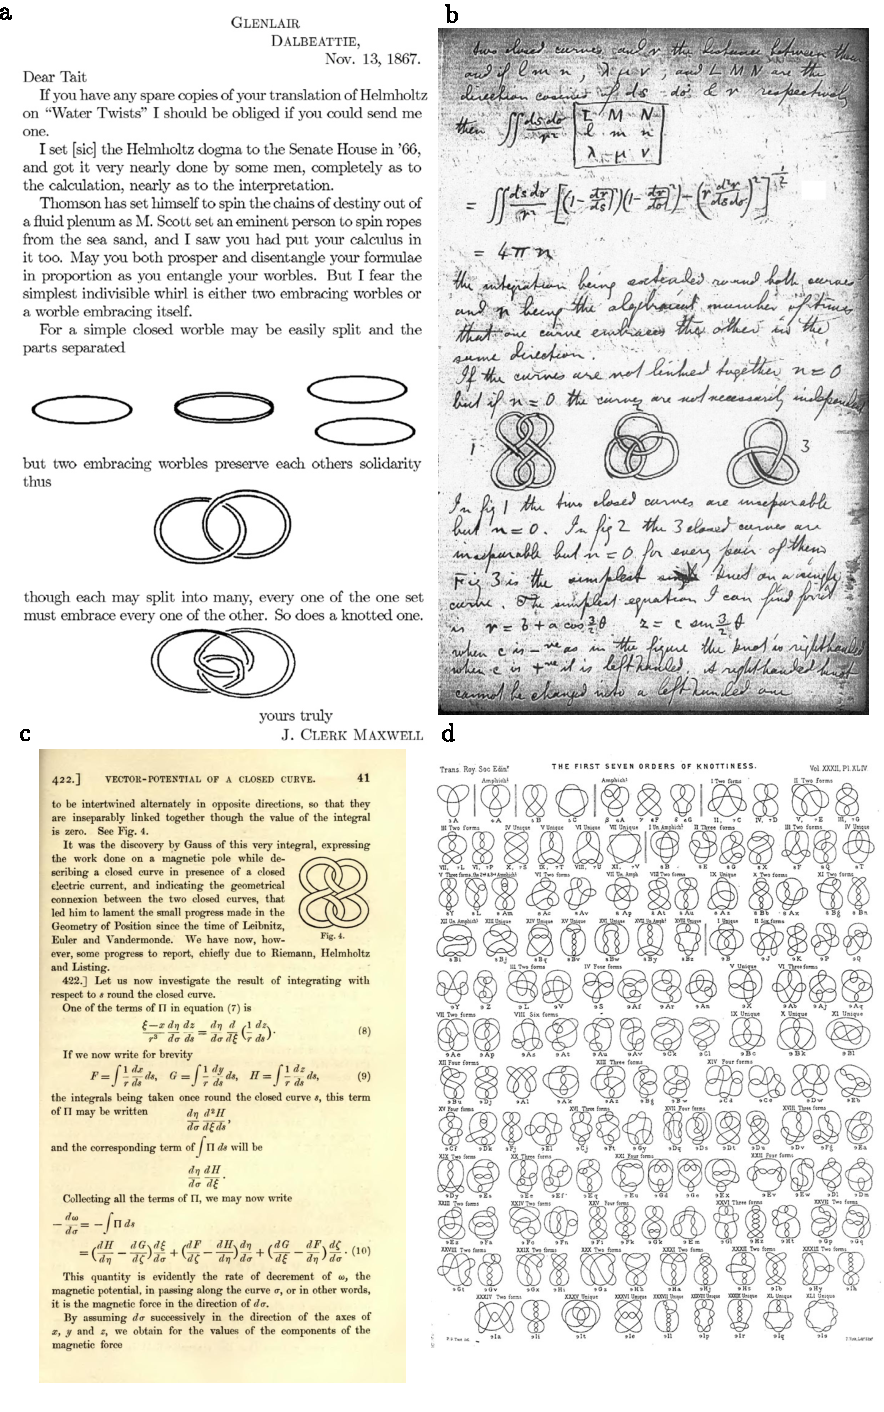
\includegraphics[width=0.9\linewidth]{\IntroductionFigures/History.pdf}
\caption{(a) 1867. Letter from Maxwell to Tait, encouraging him to ``prosper and disentangle your formulae in proportion as you entangle your worbles'' and requesting Tait's own translation of \citep{Helmholtz}. (b) 1867. Letter from Maxwell to Tait, showing a formula for Gauss's linking number alongside two links of linking number 0 and a trefoil knot. Reproduced from Ref.~\citep{Ricca2011}. (c) 1873. Page from Maxwell's \emph{A Treatise on Electricity and Magnetism}~\citep{Maxwell2}, giving a discussion of the Gauss linking number and the same example of linking number zero seen in (b). (e) 1876. The first iteration of Tait's knot tables \citep{Tait1}.}
\label{fig:History}
\end{figure}

Kelvin's ``vortex atom'' encountered difficulties in its mathematical content, its falsifiability, and a lack of contemporary experimental support \citep{KelvinMasters}. However its content, summarised as ``\textit{Physics = Geometry}'' in Ref.~\citep{KelvinAMS}, was compelling and apparently motivated Tait, in ``consideration of the forms of knots by Sir W. Thomson's (Lord Kelvin) Theory of Vortex Atoms'', to construct the first systematic tables of knots in 1876--1885, shown in figure \ref{fig:History} \citep{Tait1, Tait2, Tait3}. Tait's articles, alongside a ``very remarkable essay by Listing ... and an acute remark made by Gauss ... with some comments on it by Clerk-Maxwell''~\citep{Tait1} form the initial studies in what is now the mathematical field of knot theory \citep{Lickorish1997}. Maxwell himself, although not an active contributor to vortex atom theory, had a clear interest in the ideas, encouraging Tait in a letter in 1867 to ``prosper and disentangle your formulae in proportion as you entangle your worbles'' (figure \ref{fig:History}). Indeed the ``comments by Clerk-Maxwell'' referred to by Tait are in fact Maxwell's re-derivation of Gauss's linking number, as presented in his \textit{A Treatise on Electricity and Magnetism} \citep{Maxwell2} in 1873, about which we will have much more to say in \S\ref{ch:Maxwell}. 

Despite forming the starting point for modern knot theory, the knotted structures above are quite different to those found in your shoelaces, or in the world of art and design outside the physics department. Rather than a single knotted curve, we have a continuous fluid in whose structure the knot is encoded, and from which dynamical properties of the knot (its motion, stability, a spectrum of vibrational modes etc.) may be derived. More precisely, we have a concentrated tube of vorticity in the fluid, tied into the shape of a knot. Helmholtz's laws of vortex motion \citep{Helmholtz} show that, in a perfect (frictionless) fluid this tube of vorticity is `frozen in' to the fluid, unable to dissipate or cross itself. In an idealised vortex atom, the radius of this tube would tend to zero, with the vorticity contained inside becoming infinite, and we would have a singular linelike structure, tied into a knot and embedded into a continuous three dimensional medium. This structure is our first example of what is called a \emph{knotted field}. There is no strict definition of what constitutes of a knotted field, but a sensible operational one is that they are physical fields containing knotted, linked, or otherwise topologically interesting structure, and that this structure has some interplay with the behaviour of the whole field. As we shall see, such fields are certainly not confined to fluids.

The disconnect between a knotted curve and a knotted field is reflected in Tait's work, which mentions Kelvin's Vortex Atoms briefly as motivation, but focuses in substance on ``the investigation of the essentially different modes of joining points in a plane'' \citep{Tait1}. As knot theory developed, its initial connections to hydrodynamics and electromagnetism were further abandoned. One also notes that despite the wonderful knot tables produced by Tait (figure \ref{fig:History}) and the reliance of vortex atom theory on knotted and linked vortices, there is no mention above of any experimental evidence of vortices tied in nontrivial knots. 
\begin{figure}[htbp]
\centering
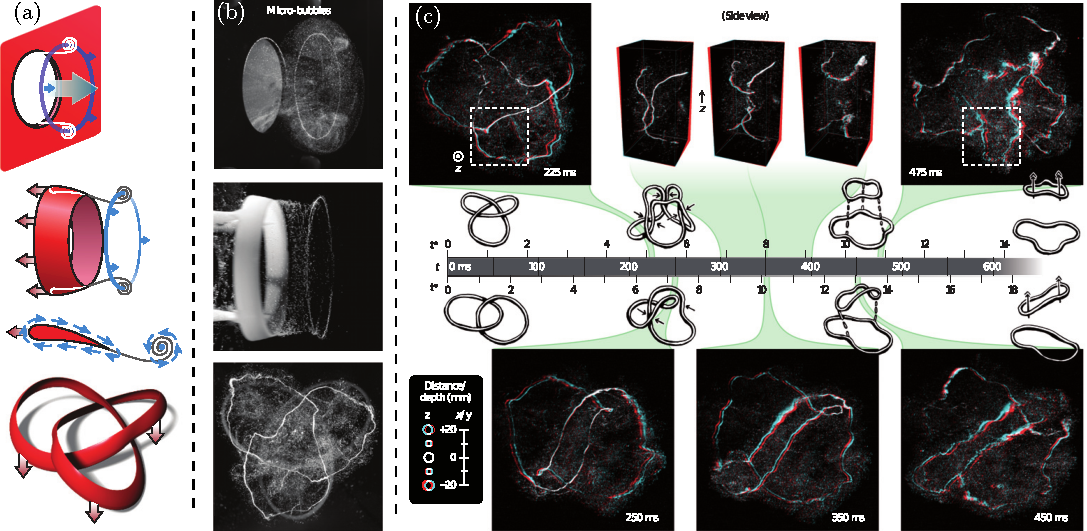
\includegraphics[width=1 \linewidth]{\IntroductionFigures/Irvine_Figs1_3.pdf}
\caption{The first experimental construction of fluid knotted vortices, in 2013. (a) Experimental methods for making knotted vortices. The hydrofoil (bottom three panels) is most successful. (b) Vortices produced in water from the designs of panel (a). Microbubbles track the vortex. The mean radius of the ring is $40$mm, of the trefoil $45$mm. (c) Timelines showing the evolution of a trefoil knot (top) and Hopf link (bottom) in three dimensions. In contrast to ideal fluids, we see progressive reconnections and simplification of the links. Figures reproduced from Ref.~\citep{Kleckner2013}.}
\label{fig:Irvine}
\end{figure}

The first experimental construction of nontrivial knotted fluid vortices came 146 years after their initial theoretical investigation, from the Irvine lab in 2013. We show in figure~\ref{fig:Irvine} several remarkable figures reproduced from Ref.~\citep{Kleckner2013}, in which Kleckner and Irvine tied a single vortex loop in water into a trefoil knot, the simplest nontrivial knot, as well as linking two vortex loops together (Kelvin's proposed model for a sodium atom), before tracking their full three-dimensional evolution. Ref.~\citep{Kleckner2013} is a notable example of a more general trend; over the past $\sim10$ years knotted fields have gone from being purely theoretical constructions to being experimentally realisable in a number of systems, and though originally conceived of in fluid dynamics, modern applications are not limited to this context; they have been realised as nodal lines of optical beams~\citep{Dennis2010}, as disclinations in nematic liquid crystals~\citep{Tkalec2011,Tasinkevych2014,Copar2015} and as spinor Bose-Einstein condensates~\citep{Hall2016}. In the following sections we will review the state of modern experiment and theory on knotted fields, beginning with fluids and superfluids, in some sense the most developed case, before moving on to parallel developments in liquid crystals and excitable media, which directly underlie the work presented in \S \ref{ch:FitzHughNagumo} and \S \ref{ch:TwistBend} in this thesis; these example are certainly not exhaustive, and focus on `soft matter' systems, a point we shall discuss at the end of the chapter. We shall see that the subject has broadened considerably since Kelvin's atoms and his contemporaries' study of fluids. There will be a commonality of ideas between the different disciplines mentioned above, but also genuine differences.
\section{Modern knotted fields: fluids}
\label{sec:Fluids}
With the decline of Kelvin's vortex atom theory and the development of knot theory away from its hydrodynamic origins, a resurgence of interest in knotted fields might be dated to the years 1958-1969, with Moreau and Moffatt's seminal papers on helicity in ideal fluids \citep{Moreau1961,Moffatt1969}, preceded by analogous results in magnetohydrodynamics by Woltjer \citep{Woltjer1958}. Focusing on the ideal fluid, both Moreau and Moffatt independently demonstrated that the helicity

\begin{equation}
    \mathcal{H} = \int {\bf u} \cdot {\boldsymbol{\omega}} \ d^3 \bf r,
\end{equation}
where ${\bf u}({\bf r},t)$ is the fluid velocity and $\boldsymbol{\omega} = \nabla \times \bf u$ is the vorticity \citep{Saffman1992}, is conserved under the Euler equations of ideal flow. Moffatt in particular gave this invariant a topological interpretation: it measures the linking of vortex tubes within the fluid. Given a fluid where $\boldsymbol{\omega}$ is concentrated along discrete sets of curves $C_i$, Moffatt showed that
\begin{equation}
    \mathcal{H} = \sum_{i,j}\Gamma_i \Gamma_j  Lk(C_i,C_j) 
\label{eq:OriginalHelicity}
\end{equation}
where $\Gamma_i$ is the vorticity flux along curve $C_i$, and $Lk(C_i,C_j), i\neq j$, is the Gauss linking number between curves $C_i, C_j$ (this interpretation of helicity actually extends to the case where the vorticity is not concentrated along a finite set of curves, but is distributed throughout the fluid \citep{Arnold1999}). The meaning of $Lk(C_i,C_i)$ will be clarified below. Figure~\ref{fig:Moffat} shows several examples of vortex tubes with different linking numbers and hence helicities. Seen in this light, the conservation of helicity is a direct consequence of Helmholtz's laws of vortex motion, and is equivalent to the statement that initially linked vortex tubes remain so; in some sense it is remarkable that the result was not known to Kelvin and Maxwell.
\begin{figure}[htbp]
\centering
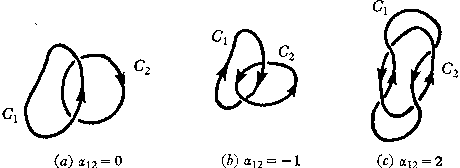
\includegraphics[width=1 \linewidth]{\IntroductionFigures/Moffat.pdf}
\caption{Three examples of links with different linking numbers. In the figure, $Lk(C_i,C_j)$ is denoted $\alpha_{ij}$. Figure reproduced from Ref.~\citep{Moffatt1969}.}
\label{fig:Moffat}
\end{figure}

When vorticity is not concentrated along a singular curve but distributed in a thin vortex tube, there is additional internal structure --- one imagines a ribbon (figure~\ref{fig:RibbonMontage}(a)), or braided rope (figure~\ref{fig:RibbonMontage}(b)). Flux lines may wind around the centre-line of this tube as in figure \ref{fig:RibbonMontage}(b), endowing it with a second linking number, the self-linking number, which measures the linking of any flux line with the curve centre-line. Incorporating this structure into the helicity count we find \citep{Moffat1992}
\begin{equation}
    \mathcal{H} = \sum_{i,j, i\neq j}\Gamma_i \Gamma_j  Lk(C_i,C_j) + \sum_{i} \Gamma_i^2 SL(C_i), 
    \label{eq:HelicityCount}
\end{equation}
where $SL(C_i)$ denotes the self-linking of each curve $C_i$ with its implicitly assumed ribbon. Defining $Lk(C_i,C_i) := SL(C_i)$ this expression reduces to~\eqref{eq:OriginalHelicity}. In Ref.~\citep{Moffatt1969} Moffatt does not explicitly consider a vortex tube, but nevertheless defines a `self winding number', which with the benefit of hindsight one interprets as the self-linking number of the simplest kind of tube, one made up of a family flux lines running parallel to one another. As we shall see below, that the flux lines are locally parallel does not imply $SL(C_i) = 0$.
\begin{figure}[htbp]
\centering
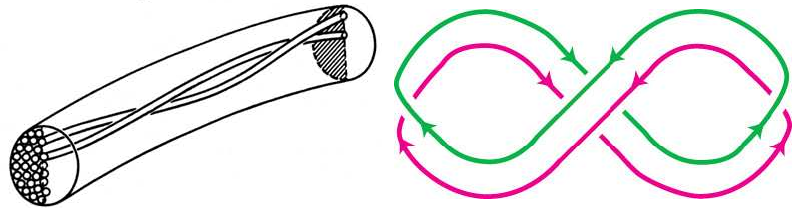
\includegraphics[width=\linewidth]{\IntroductionFigures/RibbonMontage.pdf}
\caption{A curve with internal structure: ribbons and tubes. (a) A ribbon, defined by a centre-line (pink, say) and a second offset curve (green). The diagram is a projection of the ribbon living in three dimensions, and each crossing may be annotated as either a twist $Tw$ or writhe $Wr$ crossing, depending on its local (green across pink, no pink across pink) or nonlocal (green across pink + pink across pink) nature. The total count gives a self-linking number for the ribbon; see~\eqref{eq:Count}. (b) A twisted tube, in which one particular `filament' may be arbitrarily chosen to define a ribbon. This is the situation in vortex tubes. Figures reproduced (modified) from Refs.~\citep{Dennis2005,Moffat1992}.}
\label{fig:RibbonMontage}
\end{figure}
\subsection{C\u{a}lug\u{a}reanu's theorem, real fluids}
Given a ribbon diagram like figure~\ref{fig:RibbonMontage}(a), the self-linking number may be further decomposed as
\begin{equation}
    SL = Tw + Wr.
    \label{eq:Count}
\end{equation}
The first term, the twist $Tw$, counts the local crossings of the ribbon over its centre-line. The second term, the writhe $Wr$, counts non-local crossings of the ribbon over distant parts of the centre-line. In figure~\ref{fig:RibbonMontage} each crossing of the ribbon over its centre-line is annotated with the nature of its contribution. Note that the $Wr$ count is actually independent of the choice of ribbon. For different diagrams of the same knotted ribbon each of these contributions varies, but their sum $SL$ does not. Averaging over also possible diagrams, i.e. all possible projections of the genuine three-dimensional curve, one obtains integral formulae for twist and writhe, and in this form the result~\eqref{eq:Count} was first discovered by Georges C\u{a}lug\u{a}reanu \citep{Calugareanu1959,Calugareanu1961} (the interpretation of it given above is however due to Ref.~\citep{Dennis2005}). C\u{a}lug\u{a}reanu's Theorem is an important and influential result, finding application in Mathematics~\citep{White1969,Adams2004,Aldinger1995}, Physics~\citep{Moffat1992, Goldstein1995, Berger2006}, Biology~\citep{Fuller1978, Winfree1983, Sumners1995} and beyond. It is of potential relevance whenever one studies the properties of a curve with some internal structure, and so it naturally appears frequently in the study of knotted fields. It will play a role in the curve dynamics studied in \S\ref{ch:FitzHughNagumo}, in conservation laws encountered in \S\ref{ch:TwistBend} and, in its close connection to Maxwell and Gauss's work on linking numbers and electromagnetism, in \S\ref{ch:Maxwell} as well. For the purposes of the current discussion it enables us to speak of writhe helicity $Wr$ and twist helicity $Tw$, two separate contributions to the total helicity count. All three modes of helicity storage are shown in figure~\ref{fig:Irvine2}(a). Assuming all vortices in the system have the same flux $\Gamma$ we have that
\begin{equation}
 \mathcal{H} = \Gamma^2\sum_i \sum_{j \neq i} Lk(C_i,C_j) + Tw(C_i) + Wr(C_i).\label{eq:twistpluswrithe} 
\end{equation}
To return again to Moffatt's original result \eqref{eq:OriginalHelicity}, a locally parallel bundle of tubes has $Tw(C_i) =0$, and only contains writhe helicity, as in the $Wr$ component of figure \ref{fig:Irvine2}(a) --- in other words here $SL(C_i) = Wr(C_i)$. In this case \eqref{eq:twistpluswrithe} reduces to \eqref{eq:OriginalHelicity}. Consistent with this fact, $Wr(C_i)$ may be computed from the curve $C_i$ only, without the need to explicity consider a tube at all (further, the integral formula for the Gauss linking number reduces to the integral formula for writhe when the curves involved coincide \citep{Moffat1992}), and so if one neglects internal tube structure they will pick up the $Wr$ but not the $Tw$ contributions to helicity; this is referred to as the centre-line helicity $\mathcal{H}_c := Lk +Wr$ \citep{Scheeler2014}.

In a real (viscous) fluid, helicity is not \emph{a priori} conserved. The question of whether it is in practice, and the mechanism of its dissipation, are areas of active research \citep{Kleckner2013, Scheeler2014,Scheeler2016}. Naively, one expects the reconnections shown in figure~\ref{fig:Irvine} to be accompanied by jumps in the value of helicity. Ref.~\citep{Scheeler2014} measured the centre-line helicity $\mathcal{H}_c$ across reconnections in trefoil knots and Hopf links, as shown in figure~\ref{fig:Irvine2}(b).They found that $\mathcal{H}_c$ is in fact not dissipated in a reconnection, but rather transferred from $Lk$ to $Wr$. Ref.~\citep{Scheeler2016} measured all three contributions to $\mathcal{H}$ including $Tw$ in a system of unlinked rings, finding $Tw$ to be dissipated by viscosity, but the remaining contribution $\mathcal{H}_c$ preserved (figure~\ref{fig:Irvine2}(c)). Taken together the results suggest that helicity is primarily dissipated on small scales via the $Tw$ term, and not by reconnections as might have been expected --- this leads to approximate conservation of helicity over surprisingly long timescales.
\begin{figure}[htbp]
\centering
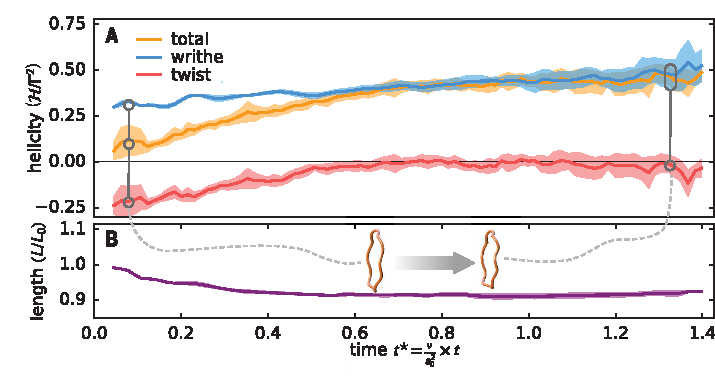
\includegraphics[width=0.9\linewidth]{\IntroductionFigures/Irvine2.pdf}
\caption{Evolution of helicity in a viscous fluid. (a) The three modes of helicity storage: linking $Lk$ of two vortex tubes, writhing $Wr$ of the centre-line of a single tube, and twisting $Tw$ of the vortex tube about the centre-line. (b) Experimental data (blue curves raw data, orange curves smoothed) tracking centre-line helicity $\mathcal{H}_c := Lk + Wr$ evolution for a trefoil knot and Hopf link, showing that $\mathcal{H}_c$ is conserved across reconnections. (c) The three contributions to helicity are experimentally tracked as a vortex ring evolves. Twist helicity $Tw$ dissipates to zero, but writhe helicity $Wr$ is conserved. (d) The experimental setup allowing the measurements shown in panel (c). Tangential flow resolution along the vortex core is enabled by impregnating an aerofoil with separated blobs of dye, which are traced over time. Figures reproduced from Refs.~\citep{Scheeler2014, Scheeler2016}. }
\label{fig:Irvine2}
\end{figure}

\subsection{Fluids as a case study}
The hydrodynamic (and magnetohydrodynamic) story of knotted fields is well developed. We have given a sketch, but the reader is invited to find more detail in reviews such as Refs. \citep{Moffatt2014, Irvine2018}. Outside of hydrodynamics the above discussion acts as a template for what one might expect in knotted fields more generally; a test case which other systems may be compared to and contrasted against. In particular, linking and self-linking of structure occur in a variety of contexts, and in analogy to~\eqref{eq:twistpluswrithe} one might seek to connect them to conserved quantities, and use them to understand the dynamics of the entire system under study. To give a brief example of a system for which this template is fruitful consider superfluids, close cousins of normal fluids described by a complex scalar field $\psi = |\psi| e^{i \phi}$ (figure~\ref{fig:SuperFluidMontage}(a)) evolving via the non-linear Schr\"odinger equation \citep{Kleckner2016}. Here vortices are given by singular lines where the circle-valued phase field $\phi$ is undefined, and about which it winds by $2\pi$. As in fluids, one may define a notion of helicity, initialise knotted vortices and study their evolution (figure~\ref{fig:SuperFluidMontage}(b)) \citep{Scheeler2014, Kleckner2016}. The definition of centre-line helicity $\mathcal{H}_c := Lk + Wr$ carries through, and its evolution turns out to be similar to that of viscous fluids \citep{Scheeler2014, Kleckner2016}; reconnections occur in similar manner, and they approximately preserve the centre-line helicity $\mathcal{H}_c$.\footnote{ \label{footnote:Seifert} Construction of the full helicity $\mathcal{H}$ is harder: the natural ribbon structure for a single superfluid vortex is given by its intersection with the surface $\phi =0$, the `Seifert framing'~\citep{Winfree1983c,MoffattBook} for which $\mathcal{H}=0$! See \citep{Salman2016,Salman2017,Kedia2018a} for a resolution to this apparent paradox. We will encounter Seifert framings again, canonically constructed by the solid angle function, in \S \ref{ch:Maxwell}.}
\begin{figure}[htbp]
\centering
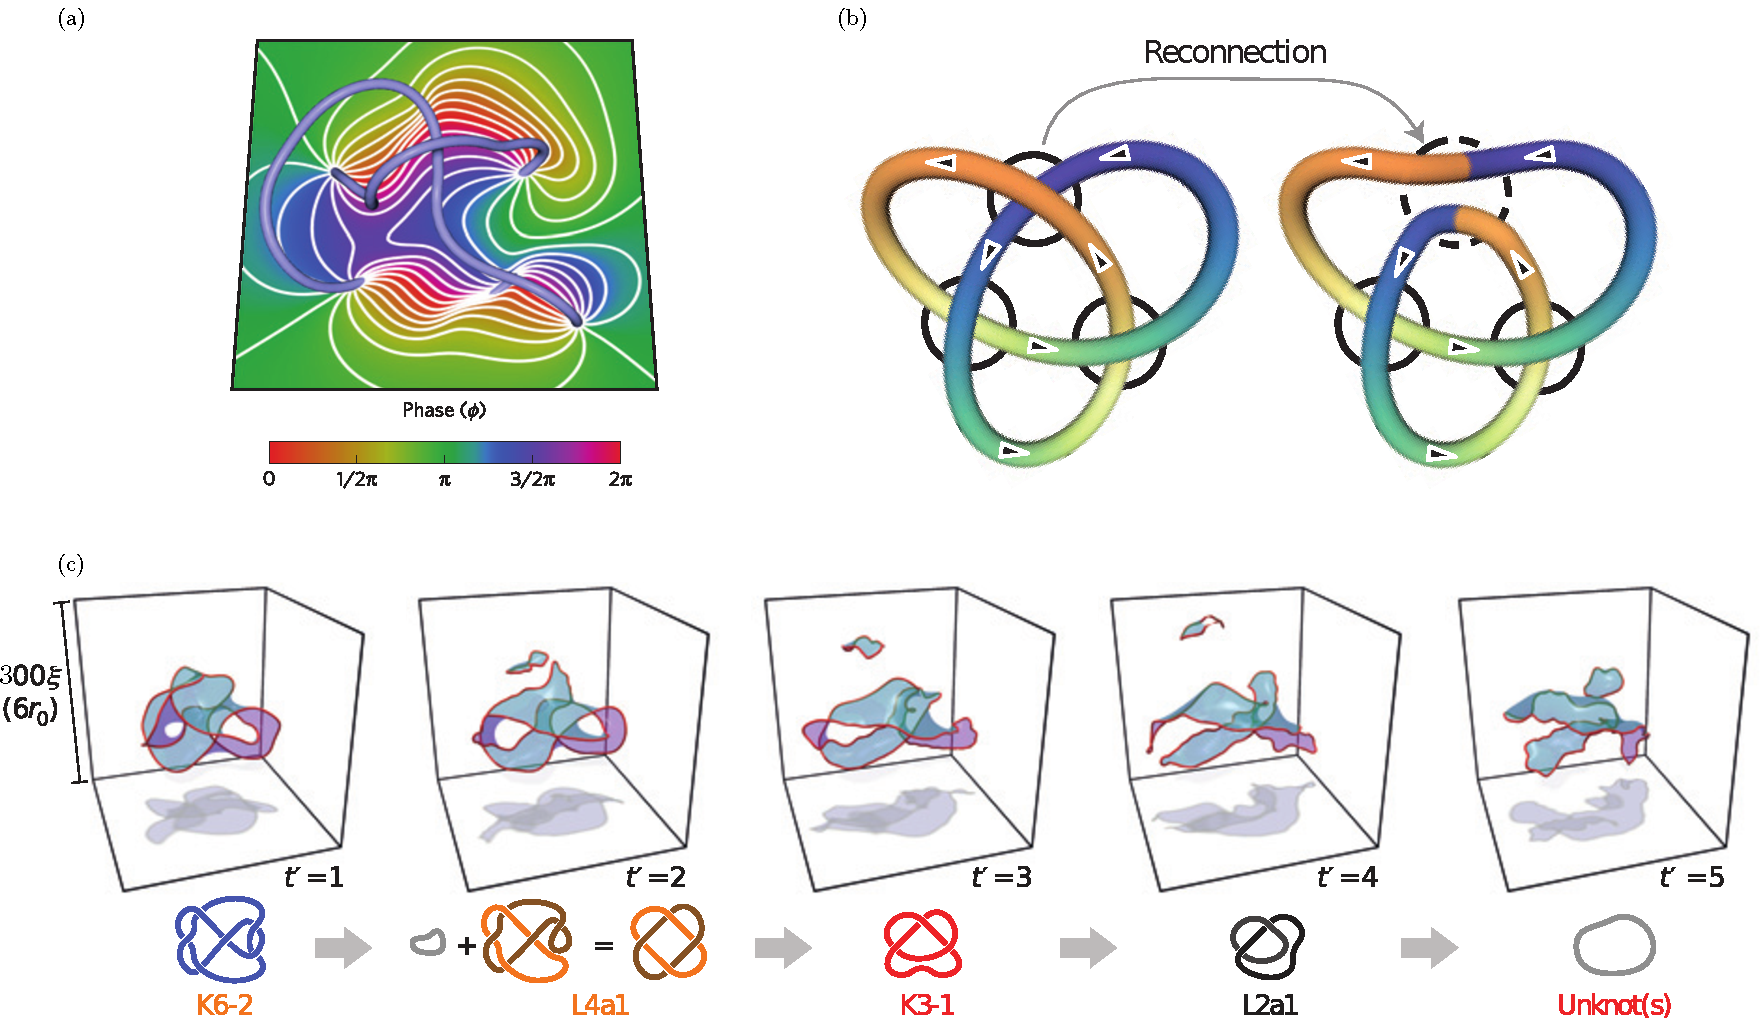
\includegraphics[width=\linewidth]{\IntroductionFigures/SuperFluidsMontage.pdf}
\caption{Evolution of superfluid vortex knots. (a) Cross section through a superfluid vortex knot (light blue curve), showing the phase field $\phi$ winding by $2 \pi$ about the vortex. (b) A schematic illustration of a reconnection. Colour is for visualisation only; note the splicing. (c) An example untying of a superfluid link into a collection of unknots by progressive reconnections. Blue surfaces spanning the knot are surfaces of constant phase. A schematic of the untying process is shown below.}
\label{fig:SuperFluidMontage}
\end{figure}

However, it is not the case that knotted fields in all other systems may be understood simply through the lens of fluids. In the following section we turn to the second experimental system with which substantial work on knotted fields has been done, the nematic liquid crystal cells of Refs.~\citep{Tkalec2011,Tasinkevych2014,Copar2015}. There will be some crossover with the discussion above, but also genuine differences, especially in the theoretical constructions involved. 
\section{Modern knotted fields: liquid crystals}
\begin{figure}[htbp]
\centering
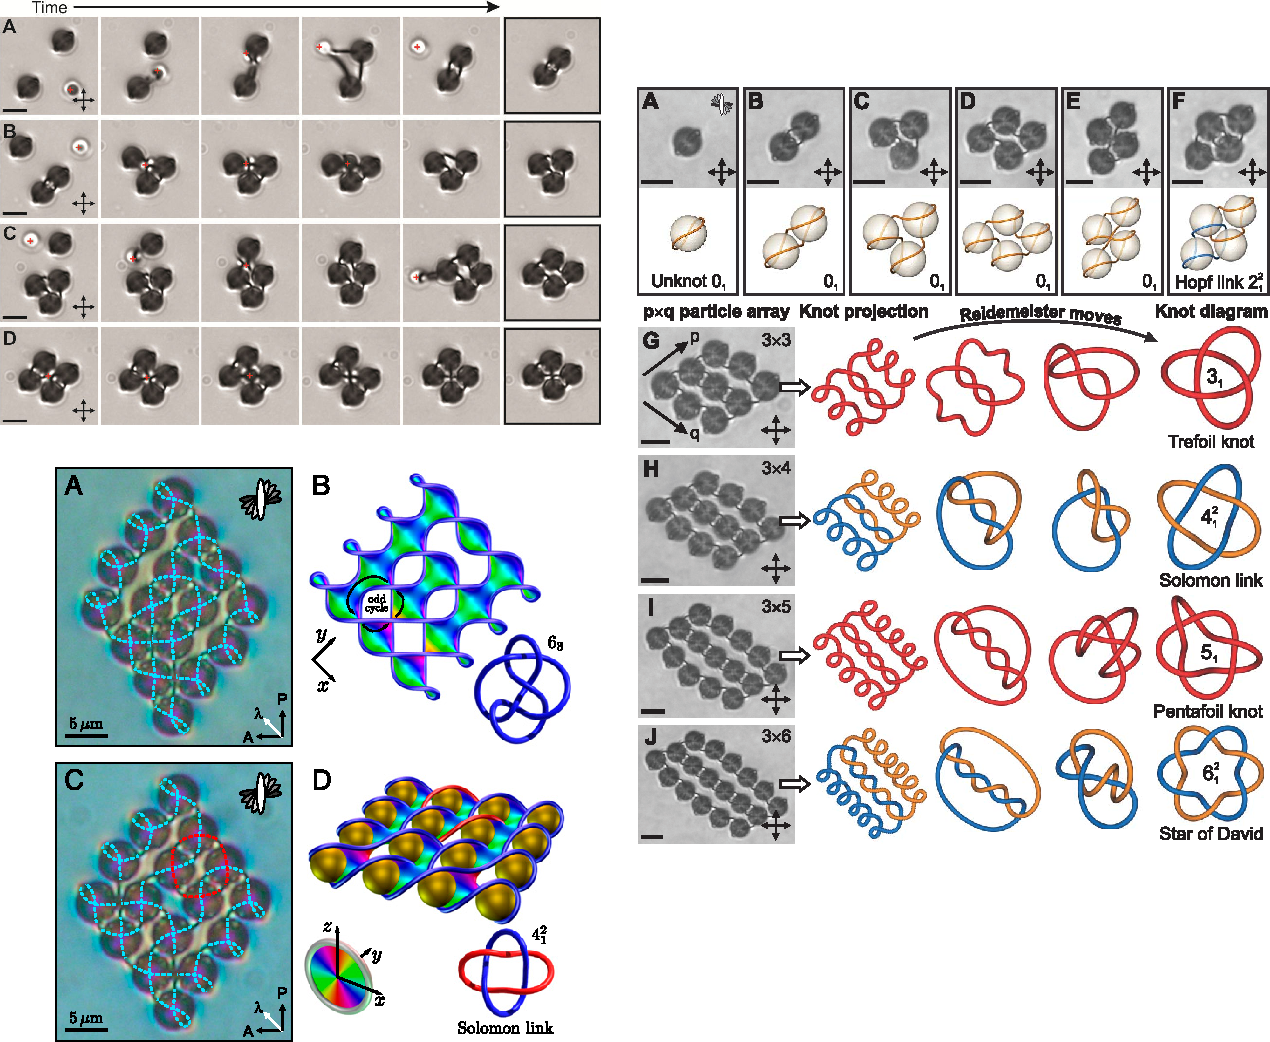
\includegraphics[width=0.8 \linewidth]{\IntroductionFigures/LiquidCrystalMontage.pdf}
\caption{Knotted disclination lines. (a) Nematic disclinations (dark curves) are wrapped around silica colloids 4.82 $\mu$m in diameter (dark spheres), initially in `Saturn's ring' configurations. Both disclinations and colloids may be manipulated by laser tweezers (red dot). The figure shows controlled assembly of an array of colloids with a single defect line wrapped about them. Black scale bar 5 $\mu$m. (b) Any knot or link may be constructed around these colloidal arrays. The figure shows the experimental assembly of a Hopf link alongside simulation predictions of its shape at each stage, as well as several other completed knots and links. (c) Within two finished links, the sense in which the director $\bf n$ is twisting is shown with colouring: the background dark blue corresponds to one handedness, with regions of light colour denoting its reversal. This visualisation allows construction of the Pontryagin-Thom (PT) surface for the link, which in turns allows homotopy classification~\eqref{eq:HomotopyClassification}. Figures reproduced from Refs.~\citep{Tkalec2011,Copar2015}.}
\label{fig:KnottedLiquidCrystal}
\end{figure}
A second experimentally constructed knotted field is shown in figure~\ref{fig:KnottedLiquidCrystal}. It is quite different to that of figure~\ref{fig:Irvine}. By including microscopic colloids a few $\mu$m wide into a thin cell of nematic liquid crystal, experimentalists~\citep{Tkalec2011,Tasinkevych2014,Copar2015} are able to force the appearance of defect lines in the material. These defects may then be manipulated with laser tweezers, and by weaving them about an array of colloids, a knotted field encoding any type of knot or link can be constructed; unlike the fluid vortices above, these structures are stable, able to be experimentally probed in some detail. This system provides a testbed for a series of new ideas about knotted fields, but first we step back a moment and provide a brief description of what liquid crystals, defects and colloids etc. actually are.

\subsection{A brief introduction to liquid crystals}

Liquid crystals are a class of materials which possess properties associated to both liquids and solids~\citep{deGennes1992}. In their most common form, the nematic phase, they show no positional order, and flow like a liquid. However, they do show orientational order: if one attempts to twist a portion of the liquid crystal it will respond elastically, as a solid would\footnote{This is remarkable: imagine your surprise if, upon attempting to stir your coffee, you found it fiercely resisted your attempts to turn the spoon, but was nevertheless happy to be poured down the sink.}. The microscopic basis for this behaviour comes from the type of molecules which comprise nematics, two examples of which are shown in figure~\ref{fig:DeGennesMontage}(a)--(b); they are typically thin rods which locally align themselves along some common axis without taking on any sort of crystalline positional order. In continuum theories this orientational order is described by a spatially varying unit vector field $\bf n$, called the director, which represents an average local molecular orientation, as shown in figure~\ref{fig:DeGennesMontage}(c).
\begin{figure}[htbp]
\centering
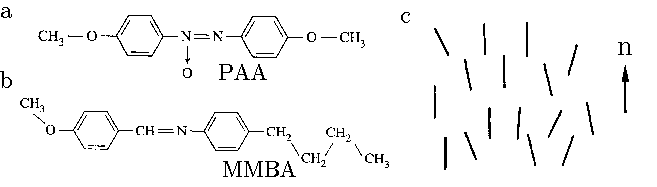
\includegraphics[width=1\linewidth]{\IntroductionFigures/DeGennesMontage.pdf}
\caption{(a,b) Two example of molecules which can form a nematic liquid crystalline phase. (a) p-azoxyanisole (PAA) forms a nematic between $116$--$135^\circ$C at atmospheric pressure. (b) N-p-methoxybenzylidene-p-butylanilinie (MMBA) forms a nematic between $20$--$47^\circ$C. (c) A schematic of local molecular alignment, with the director $\bf n$ giving a direction averaged over microscopic lengthscales. Figures reproduced (modified) from Ref.~\citep{deGennes1992}}
\label{fig:DeGennesMontage}
\end{figure}

The theory of their elastic distortions contains much interesting geometry which we will return to in \S \ref{subsec:Geometry}, but for an understanding of figure~\ref{fig:KnottedLiquidCrystal} we instead focus on a celebrated feature of nematics \citep{Frank1958}, their topological defects. If one shines polarised light through a thin slice of nematic placed between crossed polarisers, they will observe something like figure~\ref{fig:Disclination}~(a), a schlieren texture\footnote{The word `texture' is commonly used to describe liquid crystal configurations more generally.} \citep{deGennes1992}. Places in the sample where the director $\bf n$ is aligned with one of the two polariser directions H and V do not transmit light, leading to the dark brushes observed. One immediately notes points where the brushes meet, sometimes with two brushes leading into a point, sometimes four; a point of each type is marked in figure~\ref{fig:Disclination}(a). What is the structure of the director at these points? The confluence of dark brushes implies that, in a small circle around these points, the director winds, and that at the point itself we cannot consistently define $\bf n$; these points are topological defects, places where the order breaks down. Traversing such a circle around a point with two brushes, the director is aligned with each of H and V only once; in other words it makes only half a turn in a full circle around the defect. This observation is enough to establish that the director $\bf{n}$ must in fact be non-orientable; it should not be thought of as a vector field, but as a line field, for which $\bf n \sim - \bf n$.
\begin{figure}[htbp]
\centering
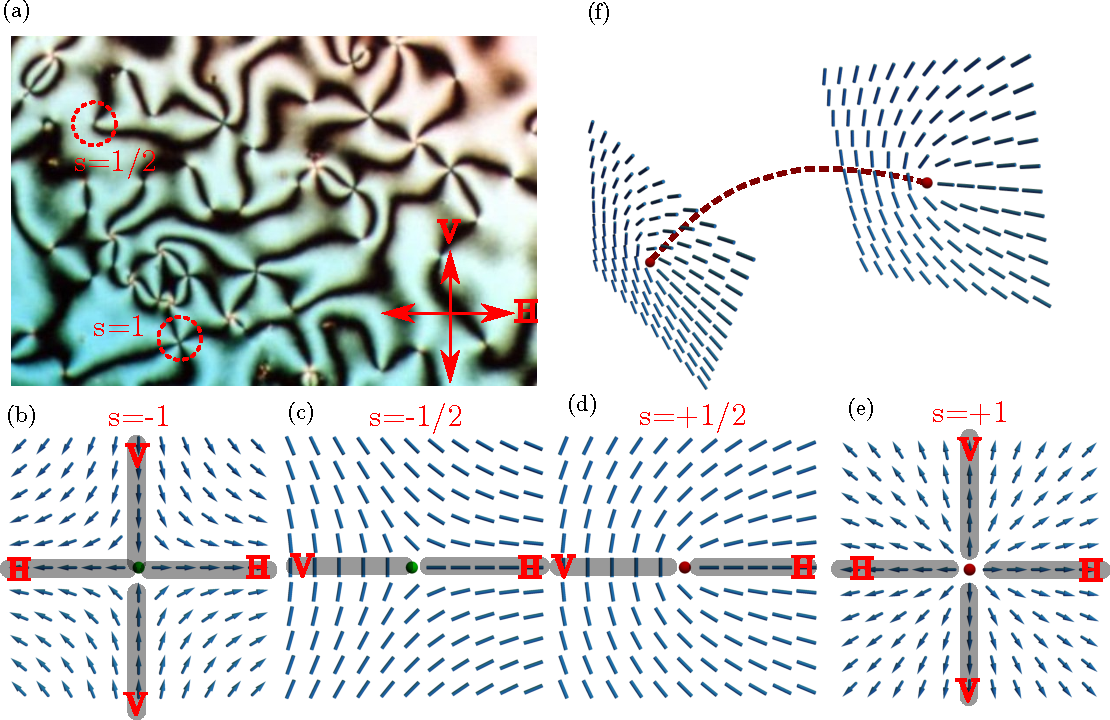
\includegraphics[width=1\linewidth]{\IntroductionFigures/DisclinationLine.pdf}
\caption{Topological defects in liquid crystals. (a) A schlieren texture, with crossed polariser directions overlaid, and defects of winding number (denoted s) $\frac{1}{2}$ and $1$ highlighted (one cannot distinguish $\pm$ from the picture alone). (b)--(e) Topologically accurate director configurations around defects of winding number $\pm \frac{1}{2}$, $\pm1$, with the schlieren dark brushes overlaid. For $\pm1$ defects it is possible to orient the director, and we have made one of the two possible choices of arrowheads. (f) Schematic of a disclination line in a three-dimensional nematic sample, with two cross sections showing local structure. Locally, there is only one type of disclination line ($\pi_1(\mathbb{R}P^2) \approx \mathbb{Z}_2$) so a winding is not given.}
\label{fig:Disclination}
\end{figure}
In figures~\ref{fig:Disclination}(b)--(e) we show qualitative configurations of the director around these defects, with their associated schlieren texture brushes. In figures~\ref{fig:Disclination}(b),(e) we have four brushes, and a line field which can be oriented; to emphasise this fact we have decorated the line field with one of the two possible choices of arrowheads. Figures~\ref{fig:Disclination}(c),(d) correspond to the non-orientable two brush case; here one cannot consistently assign arrowheads to the rods (it is worth trying to imagine doing so). Note that from a single image such as figure~\ref{fig:Disclination}(a), we cannot distinguish defects winding in a right handed sense ($+\frac{1}{2}, +1$ etc. in the figure) from left handed by counting brushes. In two dimensions these defects, also called disclinations or dis\emph{in}clinations \citep{Frank1958}, are points, but in three dimensions they are lines, transverse cross sections of which have local profiles resembling the two dimensional case; a schematic illustration is shown in figure~\ref{fig:Disclination}(f). As with fluid vortices, these disclination lines may be knotted and linked together, and the variation of the local profile along the disclination (see the cross sections in figure~\ref{fig:Disclination}(f)) provides internal structure giving rise to self-linking~\citep{Copar2011}.

\subsubsection{Experiments on knotted disclination lines}

We now return to the experiments of Refs.~\citep{Tkalec2011,Tasinkevych2014,Copar2015}. In contrast to the situation in fluids, one of the major advantages of working with liquid crystal disclinations is the control experimentalists have over them. By including microscopic silica spherical colloids (4.72 $\mu$m diameter in figure~\ref{fig:KnottedLiquidCrystal}) into a sample of liquid crystal with specific surface anchoring conditions, experimentalists may frustrate alignment of the director $\bf n$ in a controlled fashion, necessitating the appearance of disclination lines. For example, in a thin cell of liquid crystal treated to promote uniform alignment of $\bf n$ within the sample, the inclusion of a colloid with normal anchoring conditions forces the appearance of a defect line around it to cancel the colloid's topological charge (it effectively acts as a point defect) and allow $\bf n$ to relax to uniform at large distances. Two such ``Saturn's ring'' configurations may be seen in the first frame of figure~\ref{fig:KnottedLiquidCrystal}(a). Once generated, these disclinations, as well as the colloids they wrap around, may be further manipulated using laser tweezers \citep{Tkalec2011}, as shown in the remainder of figure~\ref{fig:KnottedLiquidCrystal}(a). When two of these colloids are brought together the disclinations, either spontaneously or induced by the tweezers, fuse together (figure~\ref{fig:KnottedLiquidCrystal}(a), top row). Assembling an array of these colloids and weaving the disclination lines around them, the setup of Refs.~\citep{Tkalec2011,Tasinkevych2014,Copar2015} allows targeted construction of any knot or link; examples of some possible link topologies are shown in figure~\ref{fig:KnottedLiquidCrystal}(b). This system strikingly illustrates that knotted fields have more structure than a single knotted curve --- the curve organises the entire field (in this case the director $\bf n$) around it. Figure~\ref{fig:KnottedLiquidCrystal}(c) shows the knotted liquid crystal coloured by whether the director is twisting in a right or left handed sense. We see that the disclinations separate the liquid crystal into alternately right and left handed regions. In fact this division allows construction of a surface spanning the disclinations called the Pontryagin-Thom (PT) surface \citep{ChenThesis,Chen2013}, shown as the coloured surfaces in figure~\ref{fig:KnottedLiquidCrystal}(c), which classifies the topology of this liquid crystal texture; we shall return to this surface in a moment.

Let us compare the phenomena seen here to those in \S\ref{sec:Fluids}. In contrast to fluid vortices, it is experimentally possible to stabilise liquid crystal disclinations with colloids. This fact alone leads to many differences in the character of theoretical work on them. In the absence of the stabilising colloids the disclinations will shrink under effective line tension and undergo reconnections, however there is relatively little theoretical work on possible conservation laws analogous to~\eqref{eq:HelicityCount} or on the structure of these reconnections, although some results do exist \citep{Copar2011,Machon2017}. In this sense the dynamics of these knotted fields is less understood than is the case in fluids. It turns out, however, that there is much to be understood even about the statics of knotted liquid crystal fields. In a slice of liquid crystal we saw there were many types types of defect, indexed by the winding of the director --- what of liquid crystal textures in three dimensions? More specifically, given the knotted disclinations shown in figure~\ref{fig:KnottedLiquidCrystal}, are the liquid crystal textures corresponding to them unique, or are there many inequivalent possibilities? Questions like these have a long history in liquid crystal physics which, coupled with the difference in experimental possibilities we saw above, makes some split between the character of work on knotted fields in fluids and that in liquid crystals expected.

\subsection{Homotopy theory of knotted disclinations and Pontryagin-Thom surfaces}
The traditional method of understanding liquid crystal textures containing defects is to place a measuring surface around a defect and study the possible textures on this surface, i.e. the different classes of map from the measuring surface to the space of possible values the order takes. Maps are equivalent when a continuous deformation, called a homotopy, exists between them, and as such this framework is known as the homotopy theory of defects \citep{Mermin1979,Alexander2012}. For point defects in a two-dimensional slice of nematic, this is what we did above, using a circle as our measuring surface. There, the space of possible directions $\bf n$ can point in is $S^1/\{x\sim-x\}$, the circle with antipodal points identified, also called the real projective line $\mathbb{R}P^1$. Thus the different classes of texture are reduced to the classification of maps ${\bf n}:S^1 \rightarrow \mathbb{R}P^1$ up to homotopy. This set of homotopy equivalence classes is denoted $[S^1,\mathbb{R}P^1]$. Actually computing this set is the work of algebraic topology \citep{Hatcher2012}, in which the set of homotopy classes of maps from a sphere $S^n$ into a space $X$, $[S^n,X]$, may be given a group structure after fixing a point $\star \in X$ and is called the homotopy group $\pi_n(X)$. It is found that $\pi_1(\mathbb{R}P^1) \approx \mathbb{Z}$ and thus there are infinitely many types of point defect in two dimensions as far as the traditional form of the theory is concerned; we show the four simplest in figure~\ref{fig:Disclination} but the index extends infinitely in both $+$ and $-$ senses. In three dimensions, the director takes values in $S^2/\{x\sim-x\}$, the sphere with antipodal points identified, also called the real projective plane $\mathbb{R}P^2$. Encircling a disclination line with a measuring loop as shown in figure~\ref{fig:RP2}, one finds $\pi_1(\mathbb{R}P^2) \approx \mathbb{Z}_2$, and thus there is exactly one type of disclination line, corresponding to the single nontrivial element of $\mathbb{Z}_2$\footnote{ One understands this difference by allowing the director in figure~\ref{fig:Disclination}(b,e) to buckle out of the plane of the paper, reducing these textures to the trivial one. This ``escape in the third dimension'' causes $\mathbb{Z}$ to undergo a mod 2 reduction.}.
\begin{figure}[htbp]
\centering
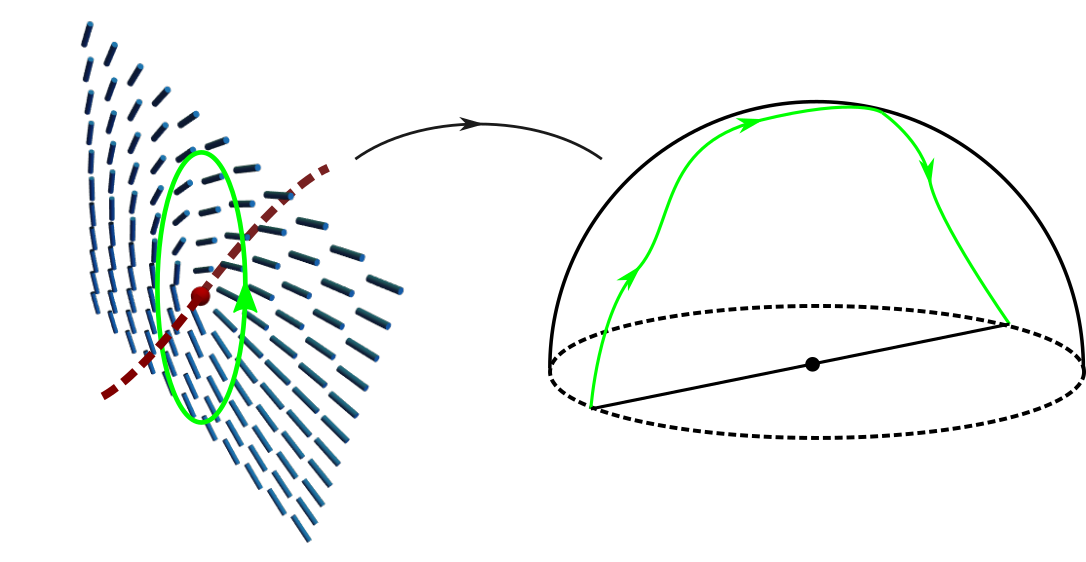
\includegraphics[width=0.9\linewidth]{\IntroductionFigures/RP2.png}
\caption{Application of the homotopy theory of defects to disclination lines. We place a measuring loop (green) around a disclination line (red curve). We then regard the director $\bf n$ (blue cylinders) as a map from this loop to the order space of the director, in this case $\mathbb{R}P^2$, modelled here as a hemisphere with equatorial points identified (pairs of red, blue, green dots indicate this identification). Homotopy theory then classifies this map as an element of $\pi_1(\mathbb{R}P^2) \approx \mathbb{Z}_2$. In this case the green curve on $\mathbb{R}P^2$ gives the single nontrivial element. If our measuring loop misses the disclination (purple) it traces a trivial path in $\mathbb{R}P^2$.}
\label{fig:RP2}
\end{figure}

A limitation of this approach is that, in only considering the texture on a specific measuring surface (in practice a sphere of some dimension) it discards information about the rest of the texture, which leads to ambiguities when considering multiple defects or more complex structures such as knotted and linked disclinations \citep{Alexander2012,Machon2014,Machon2016,MachonThesis}. A more recent, global approach \citep{Machon2014,Machon2016,MachonThesis} does not fix a measuring surface, but instead classifies maps into $\mathbb{R}P^2$ where the domain is the entire liquid crystal sample $M$ minus some set of (possibly knotted and linked) disclination lines $L$. The result is that the set of homotopy classes of the director is given by
\begin{equation}
[M-L, \mathbb{R}P^2] \approx H_1(\Sigma(L); \mathbb{Z})/\{ x \sim -x\},
\label{eq:HomotopyClassification}
\end{equation}
where $\Sigma(L)$ is the branched double cover of the link complement (its appearance in the result is a consequence of director non-orientability), and $H_1(\Sigma(L); \mathbb{Z})$ is its first homology group\footnote{An aside: if the order space is $ \mathbb{R}P^1 \approx S^1$, i.e. if one considers a phase field or a nematic confined to lie in a plane, then $[M-L, S^1] \approx H_1(M-L) \approx \mathbb{Z}$ \citep{Lickorish1997}. Such vortex lines are simply classified by their winding number, with no more internal structure.}. Without going into the details of this result, it is clear that these homotopy classes are far richer than the traditional classification scheme for disclinations would suggest, and that they depend strongly on the knot or link under consideration. To illustrate this point, in figure~\ref{fig:MachonMontage} we reproduce a `periodic table' of possible textures for $(p,q$) torus links from Ref.~\citep{MachonThesis}. Taking the simplest example from this table we see that for the Hopf link, consisting of two curves passing through each other once and given by $(p,q)=(2,2)$, there are exactly two nonhomotopic textures. Returning to the knots shown in figure~\ref{fig:KnottedLiquidCrystal}, for each knot there may be many nonhomotopic textures, and the knot diagram alone does not tell us which has actually been made. How should we extract this information, and visualise distinct textures? In figure~\ref{fig:Disclination} simple pictures of the director in the vicinity of a defect prove informative, but the same cannot be said of a swarm of sticks in three dimensions.
\begin{figure}[htbp]
\centering
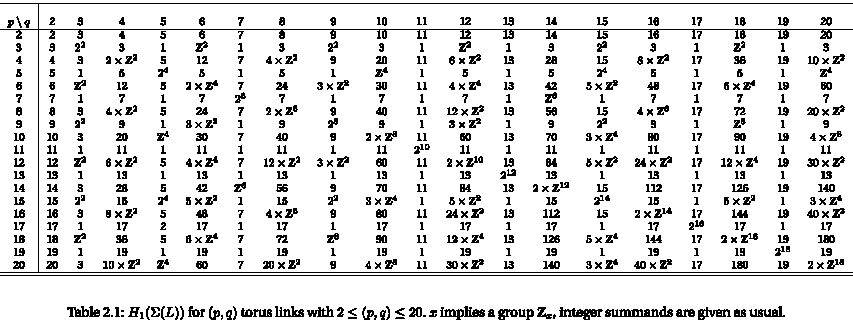
\includegraphics[width=\linewidth]{\IntroductionFigures/MachonMontage.pdf}
\caption{A `periodic table' of homotopy classes of nematic textures for $(p,q)$ torus links. Note the diversity: the sets may be finite or infinite, the number of $\mathbb{Z}$ components varies, and the number of elements in the finite component of each set may vary dramatically.}
\label{fig:MachonMontage}
\end{figure}

One solution is a construction which generalises the dark brushes of schlieren textures to three dimensions --- the Pontryagin-Thom construction \citep{ChenThesis,Chen2013,MachonThesis,AlexanderBook}. The idea is to extract the set of all points in the liquid crystal domain where the director lies in the  horizontal plane --- more precisely, perpendicular to some fixed direction in $\mathbb{R}P^2$ which we call the vertical axis. This is exactly what a schlieren textures shows in a two dimensional slice using $\mathbb{R}P^1$ instead, although schlieren textures contain some redundancy, showing us the set where the director is along some direction ($V$ in figure~\ref{fig:Disclination}(a), say) and also perpendicular to that direction ($H$ in figure~\ref{fig:Disclination}(a), the analogy to the horizontal plane in a three-dimensional texture)  --- we only really need half this data. In a three dimensional sample this `horizontal set' is not comprised of lines as in the two-dimensional schlieren texture but is a surface, the Pontryagin-Thom (PT) surface. After finding this surface, the construction is completed by colouring it according to the orientation in the horizontal plane that the director takes. An illustration of this procedure is shown in figure~\ref{fig:PT}(a). A powerful result in Algebraic Topology called the Pontryagin-Thom correspondence \citep{Milnor1997,Hatcher2012} shows that these coloured surfaces, taken up to smooth deformations (more precisely framed cobordisms), are in one-to-one correspondence with homotopy classes of maps, and so textures may be visually distinguished by their differing PT surfaces. To illustrate this fact, in figure~\ref{fig:PT}(b) we show the two distinct PT surfaces for the two nonhomotopic Hopf link textures~\citep{MachonThesis} (that they are both a single colour is an indication that representatives from both homotopy classes can be chosen with the director everywhere in the domain perpendicular to some axis, in particular one of the two horizontal axes). Returning to figure~\ref{fig:KnottedLiquidCrystal}(c), this construction provides the coloured surfaces shown; by examining the surface and the colour windings upon it, we may place the texture in one of the classes from~\eqref{eq:HomotopyClassification}. PT surfaces represent an enormous compression of information into a visually immediate form, and their utility is far from limited to disclination lines; we shall use them in our own work in \S\ref{ch:TwistBend}.

Now that we have seen some of the theoretical developments in knotted liquid crystals --- the homotopy classification, the Pontryagin-Thom construction --- let us remark again on the similarities and differences to fluids. Topological invariants play a vital role in both, linking and self-linking in fluids and homology groups of the link complement in liquid crystals. Indeed, the self-linking of liquid crystal textures will give rise to inequivalent colour windings on their PT surface and differing elements of the homotopy classification. However in contrast to fluids, where knot reconnections have been experimentally tracked and studied, there has been almost no mention of dynamics and link reconnections. When this happens, the topology of the link complement changes, and point defects may even be nucleated, perhaps a daunting theoretical task given that existing theory primarily assumes the domain is fixed, and even then finds a richness of possibility. We shall not develop this line of questioning further here, but invite the reader to consult Ref.~\citep{Machon2017} for theoretical developments in this direction. In summary, we simply remark that it is increasingly clear the world of knotted fields is far broader than fluids.

\begin{figure}[htbp]
\centering
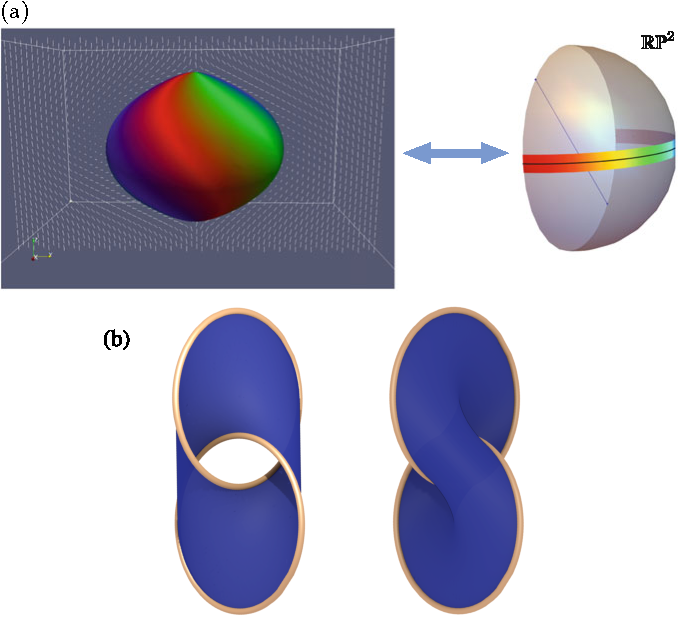
\includegraphics[width=0.8\linewidth]{\IntroductionFigures/PontryaginThom.pdf}
\caption{(a) The Pontryagin-Thom construction. The set where the director is horizontal is extracted and coloured by the angle the director makes in the horizontal plane (coloured band on $\mathbb{R}P^2$ with corresponding colours in the domain). Note that in contrast to the more standard picture of $\mathbb{R}P^2$ shown in figure~\ref{fig:Disclination} here it is `turned on its side' so that, visually, the horizontal plane through it (which one should imagine as also being the horizontal plane in the liquid crystal domain), does not coincide with the boundary of the hemisphere. The texture shown here is a topologically nontrivial one called a toron \citep{Smalyukh2010}, containing two strength $1$ point defects at its top and bottom, each detected by two rotations of the colour wheel on the PT surface. (b) Two distinct (noncobordant) PT surfaces for the Hopf link, representing the two possible nonhomotopic textures of figure~\ref{fig:MachonMontage}. Figures reproduced from Ref.~\citep{AlexanderBook,MachonThesis}.}
\label{fig:PT}
\end{figure}
\subsection{Beyond disclination lines}
The above sections focused on the knotting and nontrivial topology of disclination lines --- defects in the director $\bf n$ itself. Given the experimental focus on systems of this kind, and their direct connection to the idea of a knotted field, this is natural. However even in the absence of defects liquid crystals support an array of topological phenomena which may also be considered examples of knotted fields, although perhaps in a different sense to those discussed above. 

\subsubsection{Skyrmions and Hopfions}
\label{subsec:SkyrmionsAndHopfions}
The most well known topological feature of this kind is a skyrmion, an example of which is shown in figure~\ref{fig:HopfionMontage}(a) given by the vector field ${\bf n}(r) = \cos(\pi r) {\bf e}_z + \sin(\pi r) {\bf e}_r$ on the unit disk. Fixing the director on the disk boundary, we may wrap this texture around a sphere (compactifying the boundary to a point) at which point its topology is captured by a map ${\bf n} : S^2 \rightarrow S^2$, in other words an element of $\pi_2 (S^2)\approx \mathbb{Z}$. These textures are a well studied feature of vector and line fields in two dimensions \citep{AlexanderBook}. We are primarily interested in the properties of order in three dimensions, and as such focus on their three dimensional `cousins': Hopfions.
\begin{figure}[htbp]
\centering
\includegraphics[width=0.8\linewidth]{\IntroductionFigures/HopfionMontage.pdf}
\caption{Defect free, topologically nontrivial textures. (a) A skyrmion given by ${\bf n}(r) = \cos(\pi r) {\bf e}_z + \sin(\pi r) {\bf e}_r$, classified by an element of $\pi_2(S^2)\approx \mathbb{Z}$, here $+1$. One way to visualise this is by plotting the PT surface for the skyrmion and noting its +1 winding. (b) An experimental image of a Hopfion in nematic order, with reconstructed PT surface. It is classified by an element of $\pi_3(\mathbb{R}P^2)\approx \mathbb{Z}$, here $+1$, which may be computed via the linking number of the different stripes of colour. That each colour occurs twice reflects that fact that the order space is $\mathbb{R}P^2$ not $S^2$ (see the following panels). (c,d) A simulation of of Hopfion in vector order (order space $S^2$), with stripes of two colours picked out to aid visualisation of their linking. Note that in vector order each colour only occurs once. (d) shows a cross section of the director field corresponding to this Hopfion. (e) Recent experimental image of a Hopfion, clearly showing the telltale linking of preimages. The first panel shows a vectorised director, i.e. a choice of arrowhead has been made. In the second panel, it has not, and linking of two colours for antipodal vectors becomes linking of the same colour. (f) Polarising optical micrograph of Hopfions and other textures. Arrows showed crossed polariser directions, and the green circled cross denotes the size of the laser tweezer which manipulates them. Panels (b,e,f) reproduced from Ref.~\citep{Chen2013,Ackerman2017}.}
\label{fig:HopfionMontage}
\end{figure}
An experimental image of a Hopfion is shown in figure~\ref{fig:HopfionMontage}(b)\citep{ChenThesis,Chen2013}. The figure shows a nematic liquid crystal texture inside a three dimensional cell, where the PT surface has been constructed by extracting director orientation via three-photon fluorescence microscopy. What qualifies the Hopfion as a knotted field becomes clear on viewing this surface: each stripe of colour twists about a torus, linking each other colour exactly once --- in a Hopf link, no less. Skyrmions are classified by an element of $\pi_2(S^2)$. Hopfions are instead classified by $\pi_3(S^2)$, the third homotopy group of the sphere. Heinz Hopf famously showed that $\pi_3(S^2) \approx \mathbb{Z}$, and in doing so constructed an explicit example of a nontrivial element of this group --- the celebrated Hopf fibration. For mathematical detail on the construction of the fibration we refer to the reader to Refs. \citep{BottTuBook,AlexanderBook}, and for an excellent video of its structure we urge the reader to consult Ref.~\citep{Johnson2011}. What figure~\ref{fig:HopfionMontage}(b) shows is an experimental image of this fibration; the energetics of the liquid system favour a fixed far field nematic direction, mimicking the skyrmion boundary conditions and allowing the domain to be compactified  from $\mathbb{R}^3$ to $\mathbb{R}^3 \cup \textrm{pt} \approx {S}^3$. The nematic texture then realises a map ${\bf n}: S^3 \rightarrow \mathbb{R}P^2$, and $\pi_3(\mathbb{R}P^2) \approx \pi_3(S^2) \approx \mathbb{Z}$. The fact that the order lies in $\mathbb{R}P^2$ not $S^2$ is reflected in that fact that the fibration cycles through the colour wheel twice~\citep{Chen2013,Ackerman2017}; in figures~\ref{fig:HopfionMontage}(c)--(d) we show a Hopfion in vector order, in which each colour is only seen once. Two particular colours are picked out to make the linking clear.
\subsubsection{The geometry of vector fields}
\label{subsec:Geometry}
The linking of inverse images is the hallmark of the Hopf texture (figure~\ref{fig:HopfionMontage}(e)). However without data processing this linking is not an immediately apparent feature of the director. By contrast the knotted disclinations, and even their associated PT surface, in figure~\ref{fig:KnottedLiquidCrystal} may be clearly visualised. This is a consequence of the coupling of these topological features to the geometry, energetics and ultimately interaction with light of the liquid crystal, a coupling not present in the inverse images characterising the Hopfion in figure~\ref{fig:HopfionMontage}(e). This observation invites the question: are there `natural' features of the Hopfion, or nonsingular nematic-like liquid crystal textures in general, which can be used to infer their topology? We will explore this question, with a particular focus on a recently discovered phase of liquid crystal~\citep{Lavrentovich2018}, in \S\ref{ch:TwistBend}. The focus will be on naturally geometric structures inside the liquid crystal which also contain some topological information, and so we now discuss the geometry of nematic-like liquid crystals, and vector fields more generally. 

The fundamental geometry and energetics of nematics was encoded by Frank in 1958~\citep{Frank1958}, where he gave a free energy for their elastic distortions. We give this free energy here in a slightly nonstandard form, following Refs.~\citep{MachonThesis, Selinger2019}:
\begin{equation}
    F = \int d^3 {\bf r} \quad \frac{K_1}{2} (\nabla \cdot {\bf n})^2 +\frac{K_2}{2} ({\bf n} \cdot \nabla \times {\bf n})^2 +\frac{K_3}{2}(({\bf n} \cdot \nabla) {\bf n})^2 + \frac{K_{24}}{2} \mathrm{Tr}(\Delta)^2,  
    \label{eq:FrankFreeEnergy}
\end{equation}
\begin{figure}[htbp]
\centering
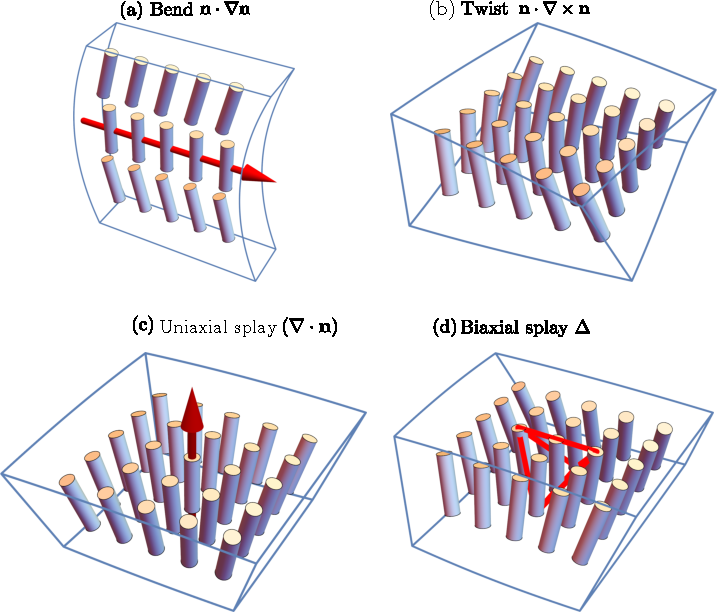
\includegraphics[width=0.7 \linewidth]{\IntroductionFigures/FrankFreeEnergy.pdf}
\caption{The four modes of director deformation: Bend, twist, (uniaxial) splay and biaxial splay. The vector plotted in (c) is the splay vector $(\nabla \cdot {\bf n}) \bf n$. Biaxial deformations, described by a rank two tensor (not a vector as in (a),(c)) are represented by a tetrahedron corresponding to the triple $\{{\bf n},\Delta_1, \Delta_2\}$, where $\Delta_i$ denotes the $i$th eigenvector of $\Delta$. Figures reproduced from Ref.~\citep{Selinger2019}. }
\label{fig:FrankFreeEnergy}
\end{figure}
where the various $K_i$ are elastic constants\footnote{These constants do not match one-to-one with those found in the standard writing of the Frank free energy; see Ref.~\citep{Selinger2019}.}. Each term in~\eqref{eq:FrankFreeEnergy} comes from a different mode of distortion for the liquid crystal, shown in figure~\ref{fig:FrankFreeEnergy}:
\begin{eqnarray}
    &({\bf n} \cdot \nabla) {\bf n} \quad \mathrm{Bend},\\
    &{\bf n} \cdot \nabla \times {\bf n}\quad \mathrm{Twist}, \\
    &\nabla \cdot {\bf n}\quad \mathrm{Uniaxial}\ \mathrm {splay}, \\
    &\Delta(\bullet) := \frac{1}{2}\Big((\bullet \cdot \nabla {\bf n})+\bf n \times({\bf n \times \bullet \cdot n)\Big)\quad \mathrm{Biaxial}\ \mathrm {splay}. 
\end{eqnarray}
Vector order has a local rotational symmetry under which the free energy~\eqref{eq:FrankFreeEnergy} must remain invariant, and indeed the above terms are exactly those combinations of gradients which respect this symmetry. More precisely, at each point in the material, the director $\bf n$ splits space into a line parallel to $\bf n$, $L$, and a plane perpendicular to it, $\xi$, $T \mathbb{R}^3 \approx L \oplus \xi$ --- an example of this splitting at a single point is shown in figure~\ref{fig:SplittingMontage}(a), and for an entire skyrmion texture in figure~\ref{fig:SplittingMontage}(b).
\begin{figure}[htbp]
\centering
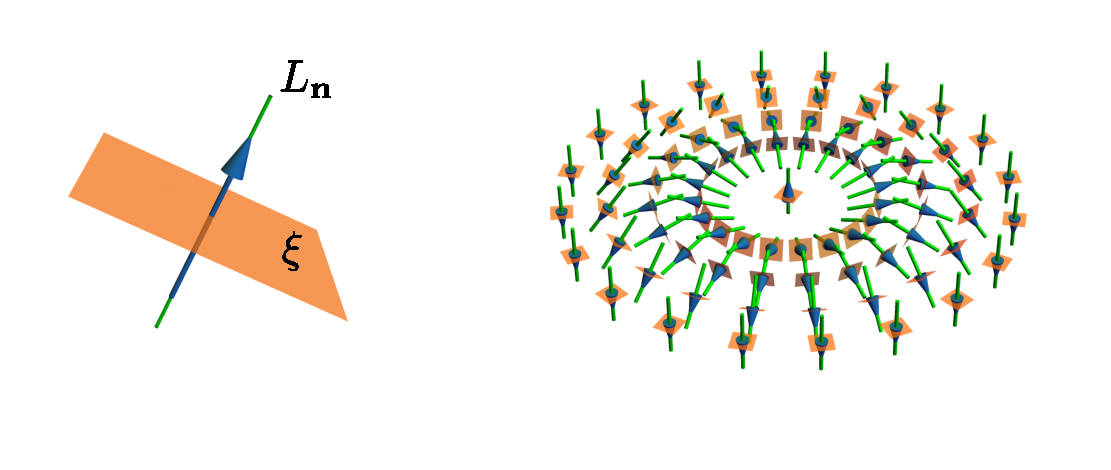
\includegraphics[width=\linewidth]{\IntroductionFigures/SplittingMontage.pdf}
\caption{ The director $\bf n $ splits space into families of lines $\L$ parallel to it, and a family of planes $\xi$ perpendicular to it: $T \mathbb{R}^3 \approx L \oplus \xi$. Panel (a) shows this splitting at one point, with the director a blue arrow, $L$ the green line and $\xi$ the orange plane. This splitting is shown for an entire skyrmion texture in panel (b). Compactifying the boundary of this skyrmion, i.e. considering the outer ring of vectors and planes to really only be one vector and one plane, the skyrmion texture is topologically the family of normal vectors to $S^2$, and $\xi$ is its tangent bundle. As such, a smoothly varying choice of vectors tangent to the family of planes $\xi$ (section of the bundle) cannot be made (it is worth imagining trying to do so: make some choice of the same fixed vector for all the outer ring of planes, and then try and extend inwards. This amounts to combing one half of the sphere and finding one cannot also comb the other).}
\label{fig:SplittingMontage}
\end{figure}
The terms appearing in~\eqref{eq:FrankFreeEnergy} correspond to the magnitudes of the irreducible components of $\nabla{\bf n}$ under the action of the rotation group $SO(2)$ on $\xi$. These piece together to give a decomposition of $\nabla {\bf n}$ in terms of gradients along $\xi$ and along $L$. Let $E_\bullet$ denote projection onto the subspace $\bullet$, and $\nabla^\bullet \bf n = (\nabla \bf n)|_\bullet$ denote restriction of the linear map $\nabla \bf n$ onto the subspace $\bullet$. Then $\nabla {\bf n}=\nabla^{L}{\bf n}E_L + \nabla^\xi {\bf n}E_\xi$, where 
\begin{align}
    &\nabla^L {\bf n}=  {\bf n}^* \otimes ({\bf n} \cdot \nabla) {\bf n}\label{eq:GradientDecompositionpar}, \\
    &\nabla^\xi {\bf n}= \frac{\nabla \cdot {\bf n}}{2}I_\xi + \frac{{\bf n} \cdot \nabla \times {\bf n}}{2} J + \Delta .
    \label{eq:GradientDecompositionperp}
\end{align}
Here $I_\xi$ is the identity transformation on $\xi$ and $J= \bf n \times \bullet$ is rotation about $\bf n$\footnote{That the splay term appears squared in~\eqref{eq:FrankFreeEnergy} is because the decomposition~\eqref{eq:GradientDecompositionpar},\eqref{eq:GradientDecompositionperp} is for vector order, not nematic order. The additional symmetry $\bf n \sim -n$ forces us to square this term. That the twist term is squared is because nematics are achiral. In a cholesteric liquid crystal \citep{Bellar2014} one has $({\bf n} \cdot \nabla \times {\bf n}+q_0)^2$, giving a linear term on expansion of the square.}. The geometry of $\nabla^\xi \bf n$ and $\Delta$ in particular has been explored in Ref. \citep{Machon2016b}. $\nabla^\xi \bf n$ describes how $\bf n$ varies as one moves in the orthogonal plane $\xi$; when $\bf n$ is the normal to a surface, -$\nabla^\xi \bf n$ is a classical object in the differential geometry of surfaces called the shape operator. The decomposition~\eqref{eq:GradientDecompositionperp} corresponds to its breakdown into an isotropic piece $I_\xi$, an antisymmetric piece $J$ and a traceless symmetric piece $\Delta$. When $\bf n$ is the normal to a surface the antisymmetric piece $J$ vanishes, and $\Delta$ is just $\nabla^\xi \bf n$ with the isotropic part removed --- the eigenvectors of $\Delta$ then coincide with those of $\nabla^\xi \bf n$ and pick out the two directions of principal curvature in $\xi$. This interpretation extends to the general case where $J \neq 0$, and the eigenvectors of $\nabla^\xi \bf n$ do not necessarily exist, explaining the name ``biaxial splay'' for its mode of distortion. The geometry of $\nabla^L \bf n$ is less well explored. It describes the bending of the director field: if one traces a single curve to which $\bf n$ is tangent, then $\nabla^L \bf n $ gives the classical curvature from the differential geometry of space curves \citep{DoCarmoBook}. A more complete account of its geometry will, in part, be the topic \S\ref{ch:TwistBend}.
 
Each of the pieces in~\eqref{eq:GradientDecompositionpar}, \eqref{eq:GradientDecompositionperp} is manifestly geometric, but they also represent topological information as canonical sections of vector bundles defined by the director. The families of lines $L$ and planes $\xi$ vary smoothly with the director, and such smoothly varying families of vector spaces are called vector bundles \citep{TuBook,MilnorStasheffBook}. The most famous example of a vector bundle, and the interesting properties they can have, is the family of planes tangent to $S^2$ called its tangent bundle $T S^2$. A smoothly varying choice of vector in each of these tangent planes is called a section of the tangent bundle (or more commonly simply a vector field), and is denoted $\Gamma (TS^2)$. Famously, the Poincare-Hopf theorem tells us one cannot `comb a sphere' \citep{Milnor1997}, in other words one cannot find an everywhere nonzero section of the tangent bundle to the sphere. This failure is connected to the topology of $S^2$; if one sums the windings of all the zeros in any such section one obtains the Euler characteristic of $S^2$. An entirely analogous result holds for any vector bundle; the zeros of a section of a vector bundle encode its Euler class \citep{BottTuBook, MilnorStasheffBook}. Returning to~\eqref{eq:GradientDecompositionpar}, \eqref{eq:GradientDecompositionperp}, $\nabla^\xi \bf n $ is a section of the bundle $\xi^* \otimes \xi$ --- it maps vectors orthogonal to $\bf n$ into vectors orthogonal to $\bf n$ --- and the bend $\nabla^L {\bf n} \in \Gamma (L^* \otimes \xi)$. Both probe the topology of $\xi$ and, loosely speaking, as $\xi$ is in one-to-one correspondence with the director $\bf n$ this topology carries over to $\bf n$. The zeros of $\Delta$, called umbilic lines in analogy to the umbilic points of the differential geometry of surfaces, have been investigated in Ref.~\citep{Machon2016b}. The zeros of $\nabla^L \bf n$, which we will call $\beta$ lines, will be the subject of \S\ref{ch:TwistBend}.

The umbilic and $\beta$ lines are natural geometric structures found in any vector field. However, they assume a particular relevance when strongly coupled to the energetics of the liquid crystal texture. One way to do this is to frustrate the liquid crystal with boundary conditions, as in the disclinations of figure~\ref{fig:KnottedLiquidCrystal}. Another is to pass to a different phase of liquid crystal, where such coupling exists. In the case of umbilic lines, this setting is the cholesteric phase \citep{Bellar2014}, in which the liquid crystal has a preference for nonzero twist; $\Delta$ turns out to be related to the axis of this twisting~\citep{MachonThesis, AlexanderBook}, and its zeros thus encode energetic frustration inside the cholesteric~\citep{Machon2016b}. For $\beta$ lines, the natural setting is a recently discovered phase of liquid crystal, the twist-bend or splay-bend nematic \citep{Lavrentovich2018}. These materials, comprised of banana shaped molecules, have an energetic preference for everywhere nonzero bend. A second focus of \S\ref{ch:TwistBend} will be on this interplay between geometry and energetics in twist-bend nematics. 

\section{Modern knotted fields: excitable media}
\label{sec:FN}

\setlength{\epigraphwidth}{5in} 
\epigraph{``In excitable media we may have a new context in which something like a vortex atom theory can live again, strangely transfigured.''}{A. T. Winfree, The Geometry of Biological Time, Chapter 9.}
\begin{figure}[htbp]
\centering
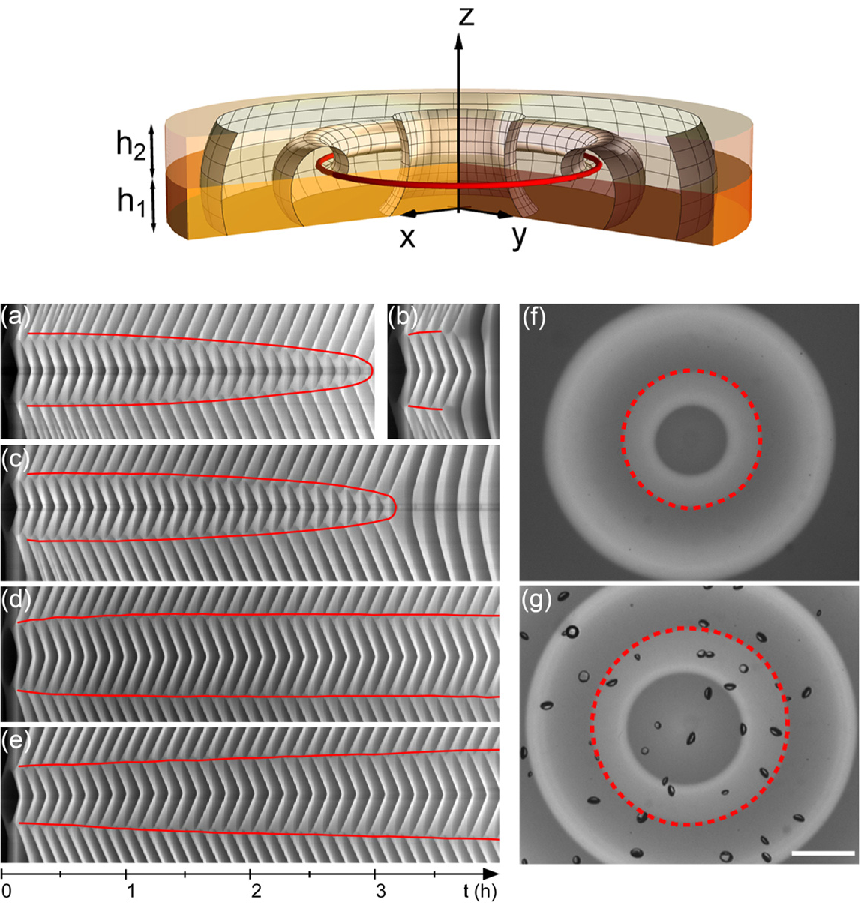
\includegraphics[width=\linewidth]{\IntroductionFigures/FNExperimental.pdf}
\caption{Top Panel: Schematic illustration of a vortex ring in excitable media. A dish of the Belousov-Zhabotinsky reagent supports an axially symmetric spiralling wave of chemical activity (meshed wavefronts) emanating from a ring shaped singularity shown in red. Bottom Panel: An experiment realising this setup. (a)--(e) shows a time series of the dish viewed side on, i.e the $x$-$z$ plane, over $4$ hours. The rotation period of the wave itself is $390$s $\approx 6$--$ 7 $ mins. In each frame, the ring appears as a pair of points with wavefronts emanating from it, which collide in the middle of the dish. Over time the ring moves, tracing the curves shown. Depending on the heights $h_1$ and $h_2$ it may shrink (a), (c), reach a steady radius (d) or expand (e). (f) and (g) show the ring from above ($x$-$y$ plane) over $3$ hours. Setting spatial scale, the white bar in (g) corresponds to $5$ mm. Figures reproduced from Ref.~\citep{Totz2015}.}
\label{fig:FNExperimental}
\end{figure}

We now come to our final example of knotted fields, those found in excitable media. We might have discussed them immediately after fluids and superfluids, and indeed we will see closer similarities to those systems than to liquid crystals. That we chose not to is a reflection of their relative lack of experimental development. By way of prelude, the modern state of affairs in these systems is that the analogy to a fluid vortex ring can be generated experimentally \citep{Steinbock2006,Azhand2014, Totz2015}. Figure~\ref{fig:FNExperimental} shows a schematic of a thick dish of the Belousov-Zhabotinsky (BZ) reagent, a medium which supports waves of propagating chemical activity. Axially symmetric waves of such activity spiral outwards from a `singular' ring shown in red --- exactly what is occurring on this ring will be discussed below. Beneath it is an experimental realisation of this setup from Ref.~\citep{Totz2015}, viewed from the side in figures~\ref{fig:FNExperimental}(a)--(e) and from the top in figures~\ref{fig:FNExperimental}(f)--(g). From the side the ring appears as a discontinuity in the emitted wavefronts, with a second such discontinuity where the fronts collide in the middle of the dish. Figures~\ref{fig:FNExperimental}(a)--(e) show stacks of snapshots of different rings evolving over time, with the overlaid red curves tracking their position. They show, firstly, that the rings stably persist over several hours, and secondly that they have their own dynamics, expanding, contracting or reaching a stable radius (the outcome may be experimentally tuned). The topological possibilities, dynamics, and organisation of the entire excitable medium by these rings are the subject of this section, and of \S \ref{ch:FitzHughNagumo}. These rings have not yet been experimentally tied in nontrivial configurations --- as we shall see in this section, such an experiment would be extremely interesting.

\subsubsection{Excitable media}

The building block of an excitable medium is an excitable oscillator, something which rests in a quiescent locally stable state but which, given a small kick, becomes excited before relaxing back to quiescence. A prototypical example is a nerve cell. Given an electrical input, the cell `fires', becoming excited, before slowly relaxing back to its resting state where it can be triggered again. An excitable medium is a continuum of these oscillators, all coupled together, in our case by diffusion of activity from one oscillator to its spatial neighbours. Such media support waves of activity, where an excitation in one oscillator triggers its neighbours to `fire' also. A pleasing example of such waves is a grass fire \citep{Winfree1983}. The oscillators are blades of grass. Their resting state is unburnt, their excited state burnt. After burning, the blades slowly grow back, able to be burnt again. A field of grass, the excitable medium, supports a wave of excitation, i.e. a moving front of grass fire. Note the front has a leading edge (the transition from unexcited to excited) and a trailing edge (the transition from excited to unexcited).

There is an enormous experimental and theoretical literature on systems exhibiting this sort of behaviour; for references see \citep{WinfreeBook}. We present a minimal mathematical model, which shall be the focus of \S\ref{ch:FitzHughNagumo}, and which provides an effective description of many more complex excitable media \citep{WinfreeBook}: the FitzHugh-Nagumo model \citep{FitzHugh1961,Nagumo1962}
\begin{equation}
\label{eq:FN}
\frac{\partial u}{ \partial t} = \frac{1}{\epsilon}\biggl(u - \frac{1}{3}u^3 -v\biggr) + \nabla^{2} u,\hspace{2em}    \frac{\partial v}{ \partial t} = {\epsilon}(u + \beta -\gamma v) ,
\label{eq:FN}
\end{equation}
Here $u(\bf {x} ,t)$ , $v({\bf x},t)$ are two real valued scalar fields, with $\epsilon,\gamma,\beta$ model parameters. The coupling which turns this system from an excitable oscillator to an excitable medium is through diffusion $\nabla^2 u$, in this instance in the $u$ variable only (although variants with diffusion in each variable also exist). The phase plane for the differential equation system without diffusion is shown in figure~\ref{fig:FN}(a), with parameter choices which will generate an excitable oscillator. The system has a fixed point $(u^*,v^*)$ (black dot), but given a finite perturbation in $u$ it will execute a large loop in phase space called the excitation-recovery loop, jumping to the upper branch of the $u$ nullcline, crawling along it until the first inflection, whereupon it jumps to the lower branch and crawls again back to the fixed point (black arrows in the figure). In the sense that a perturbation in $u$ instigates this loop, $u$ might be considered an `excitor' variable and $v$ a `recovery' variable.
\begin{figure}[htbp]
\centering
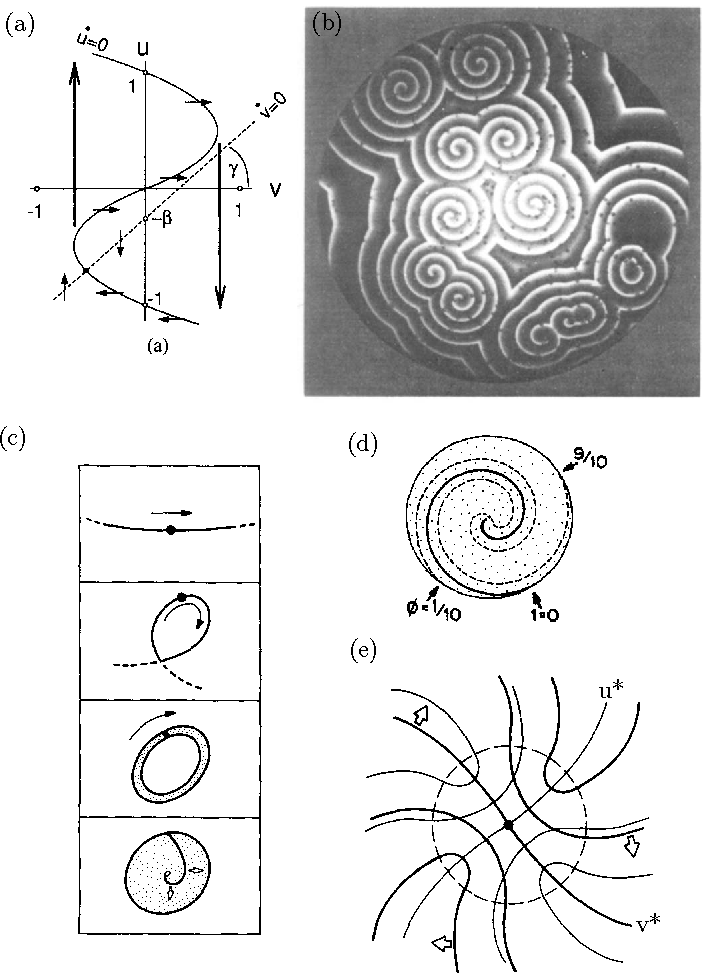
\includegraphics[width=0.8\linewidth]{\IntroductionFigures/FN.pdf}
\caption{Spiral waves in two dimensions. (a) The phase plane of the FitzHugh-Nagumo model~\eqref{eq:FN}, with $u$ and $v$ nullclines (solid and dotted curves), fixed point (black dot) and excitation-recovery loop (large black arrows) shown. This loop is topologically a circle $S^1$, and progression through a cycle of excitation-recovery can be described by a phase $\phi \in S^1$. (b) Spiral waves in a dish of the BZ reagent. (c) --(e) The anatomy of a single spiral wave. In (c) one imagines setting a pulse of excitation running around a closed loop, which gradually thickens until the propagation time around its inner edge is faster than the medium can recover from. The resulting structure is a spiral wave. (d) shows its phase description, with three example isophase spirals shown. (e) A qualitative picture of the $(u,v)$ field around a spiral wave vortex. Away from the vortex the contours are parallel, but inside they necessarily cross one another transversally. Figures reproduced from Ref.~\citep{Winfree1983}. }
\label{fig:FN}
\end{figure}

\subsubsection{The topological possibilities of excitable media}

The key topological observation is that the excitation-recovery loop is a circle $S^1$. In a portion of excitable media $M$, the state of a typical point lies somewhere on this loop, and thus we can describe the system with a map $\phi : M \rightarrow S^1$, a situation encountered before in superfluids. Concretely mapping between $(u,v)$ and $\phi$ may be achieved via something of the form $(u,v) = (2 \cos \phi - u^*, \sin \phi - v^*)$, stretching $S^1$ over the excitation-recovery loop. That the system is characterised by the phase field $\phi \in S^1$ immediately implies the potential existence of knotted and linked vortices if our domain $M$ is three-dimensional, again by simple analogy with superfluids. What makes this system so interesting is that the character and dynamics of these phase singularities are very different to what we have encountered before. 

In two dimensions these singularities are at the core of spiral waves, a collection of which are shown in the BZ reagent in figure~\ref{fig:FN}(b). The anatomy of a single spiral wave is dissected in figure~\ref{fig:FN}(c)--(e). In figure~\ref{fig:FN}(c), one imagines taking an initially thin ring of excitable medium and setting a wave of excitation running around it. If the ring is thickened, we expect some spatial variation in the wavefront--- it turns out that given isotropic diffusion in~\eqref{eq:FN} it takes the shape of an involute spiral started from the inner edge of the ring \citep{WinfreeBook}. This thickening process happily continues until the time taken for the inner edge of the wave to circulate once is comparable to the recovery time of the medium, a condition which defines a `core region', inside of which the $(u,v)$ states of points leave the excitation-recovery loop and so cannot be reliably assigned a phase $\phi$ (this is analogous to what happens inside the healing lengthscale which sets vortex core size in superfluids). A phase description in which the core is idealised to zero radius is shown in figure~\ref{fig:FN}(d), and a qualitative picture of the corresponding contours of $(u,v)$ is shown in figure~\ref{fig:FN}(e). These `rotors' periodically emanate waves of excitation which organise the entire medium, splitting it into domains separated by shock structures where two wavefronts coincide and annihilate (figure~\ref{fig:FN}(b)).
\begin{figure}[htbp]
\centering
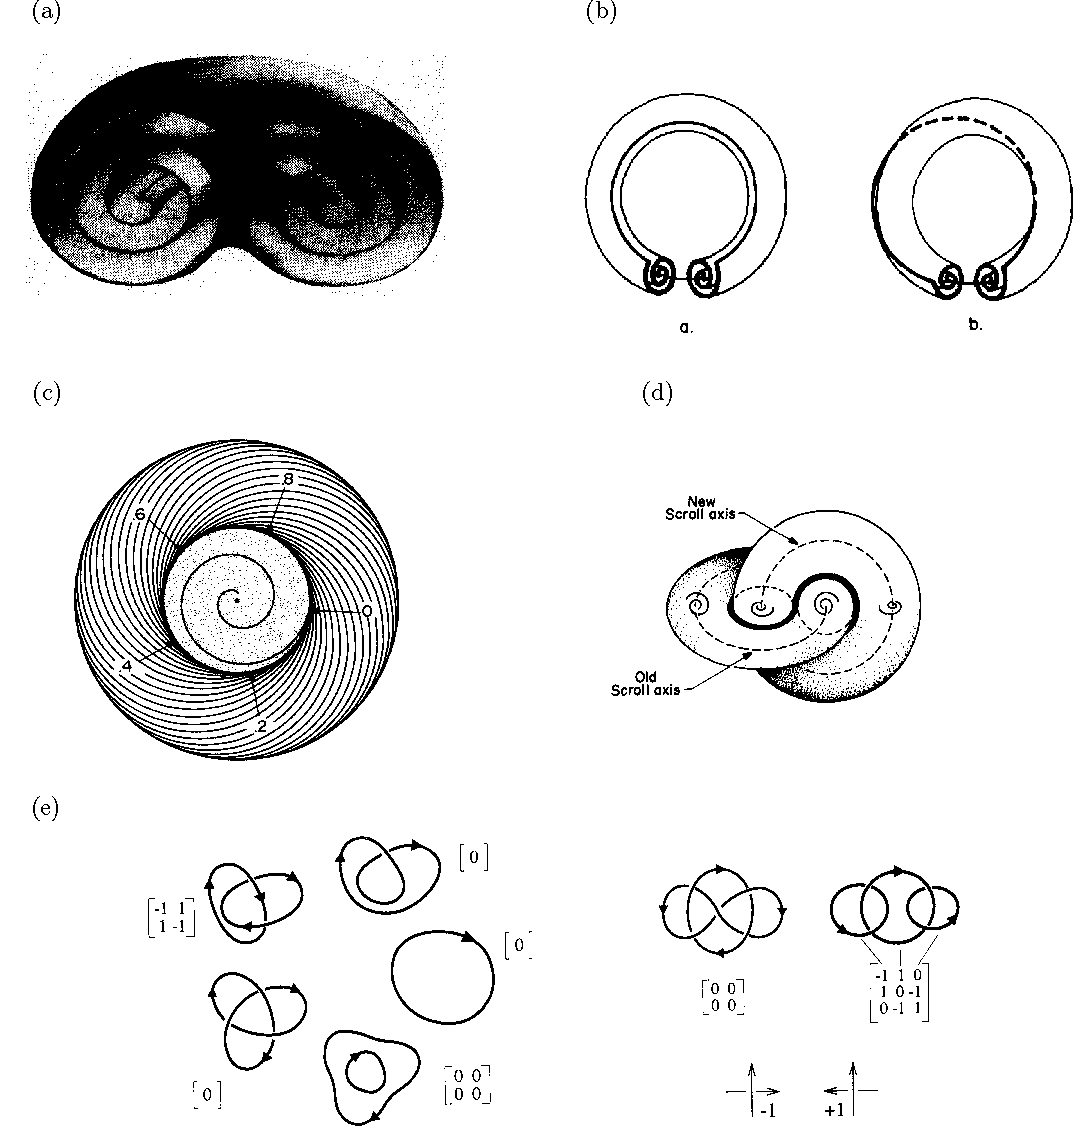
\includegraphics[width=\linewidth]{\IntroductionFigures/FN3D.pdf}
\caption{The topological possibilities of knotted vortices in excitable media. (a) A spiral wave rotated around an axis of symmetry forms a scroll wave, shown in cross section with wavefronts in grey. This is the system realised in figure~\ref{fig:FNExperimental}. (b) Cutting a scroll wave, putting a full turn of each phase contour into it, then gluing back together. (c,d) This twisted scroll ring has a full cycle of phase around its equator (points $0$ through $8$ in panel (c)), necessitating the existence of a second twisted scroll ring linking the first, shown in (d). (e) Two groups of knotted vortices, with transmutations topologically allowed between neighbouring elements of each group. The matrices shown have $(i,j)$th element $Lk(C_i,C_j)$, where $Lk(C_i,C_i):= SL(C_i)$. Note each row (and column) sums to zero, an expression of~\eqref{eq:SelectionRule}. Figures reproduced from Refs.~\citep{Winfree1983, Winfree1983b, Winfree1990}.}
\label{fig:FN3D}
\end{figure}

In three dimensions, we have a linelike phase singularity, a vortex filament, emitting `scroll waves'. The geometric and topological possibilities of linked and knotted vortex filaments were first investigated in a series of papers by A.T. Winfree and S. Strogatz \citep{Winfree1983, Winfree1983b, Winfree1983c, Winfree1984}. The simplest possibility is for the filament to close into a ring, emitting axially symmetric waves which fill space as shown in figure~\ref{fig:FN3D}(a). This is the situation encountered experimentally in figure~\ref{fig:FNExperimental}. However, Winfree and Strogatz demonstrated numerous other possibilities. For example, we once again have internal structure along the singularity, in this case the angle the $\phi=0$ contour (say) makes with the filament in successive cross sections along it, which opens up the possibility of self-linking. The simplest such scenario, a twisted scroll wave, is shown in figures~\ref{fig:FN3D}(b)--(c). Focusing on figure~\ref{fig:FN3D}(c), we note that such twisting implies a full cycle of phase about a line threading the hole in the ring. In other words, a second phase singularity must exist along this line too! Closing this line into a second loop, we obtain figure~\ref{fig:FN3D}(d); two scroll rings, each with linking and self-linking number (+)1. Winfree and Strogatz extend this line of reasoning in a manner similar to that of Moffatt in Ref.~\citep{Moffatt1969} to derive a topological selection rule on allowed configurations of knotted vortices: 
\begin{equation}
    0 = \sum_{i,j, i\neq j} Lk(C_i,C_j) + SL(C_i), \quad \forall i. 
    \label{eq:SelectionRule}
\end{equation}
This rule has a similar feel to the helicity count of~\eqref{eq:HelicityCount}, but its content is slightly different. It is a condition each knotted loop in a link must satisfy in order for the whole to exist. In fact a separate continuum definition of a helicity has been given \citep{Trueba2009} but it is currently not clear (to me at least) how the concepts interlink; it is an interesting question for further study \footnote{~\eqref{eq:SelectionRule} corresponds to giving the link its Seifert framing~\citep{Winfree1983c,MoffattBook}, already seen in superfluids in footnote~\ref{footnote:Seifert}, for which $\mathcal{H}=0$.}.

\subsubsection{The dynamical possibilities of excitable media}

Provided the topological constraint~\eqref{eq:SelectionRule} remains satisfied, there is no reason link reconnections cannot occur, as they do in the other systems we have discussed. In figure~\ref{fig:FN3D}(e) we show two groups of allowed knotted vortices, and within each group transmutations are topologically allowed. As Winfree and Strogatz note, questions of whether or not they actually occur in a given excitable medium ``probably depend sensitively on the exact kinetics of the medium'' \citep{Winfree1984}. In the experiment of figure~\ref{fig:FNExperimental}~\citep{Totz2015} we saw that these vortex lines are not merely static emitters of wavefronts, they have their own dynamics, and one has no \emph{a priori} reason to expect these dynamics to preserve topology. What is absolutely remarkable is that, in a certain parameter regime in the FitzHugh-Nagumo model, it was found that they do \citep{Winfree1990,Henze1993}. Using $\epsilon = 0.3, \beta = 0.7, \gamma=0.5$, a stable vortex ring was found in \citep{Courtemanche1990}, shown in figure~\ref{fig:FNKnots}(a), followed by a stable trefoil knot \citep{Henze1991}(in a slightly different kinetics) and then a variety of apparently stable knots and links \citep{Henze1993} summarised in figure~\ref{fig:FNKnots}(b). An account of this first period of development may be found in Refs.~\citep{Winfree1990, WinfreeBook,WinfreeChapter}. Subsequent work \citep{Sutcliffe2003} confirmed a wide basin of stability for the trefoil knot and the Hopf link over substantially larger time periods than the original trefoil simulations were run for. More recently, Maucher and Sutcliffe \citep{Maucher2016} showed that the FitzHugh-Nagumo dynamics is even capable of simplifying a tangled unknot into a unique canonical round form, as well as demonstrating stable forms for more complex knots --- the figure-eight and torus links in certain geometries \citep{Maucher2017}. A simplification of an unknot with 13 crossings in projection is shown in figure~\ref{fig:FNKnots}(c), with a cross section to show the associated wavefield in figure~\ref{fig:FNKnots}(d) (one might compare to figure~\ref{fig:FN}(b)). The stable torus and figure-eight knots with associated minimal lengths are shown in figure~\ref{fig:FNKnots}(e).
\begin{figure}[htbp]
\centering
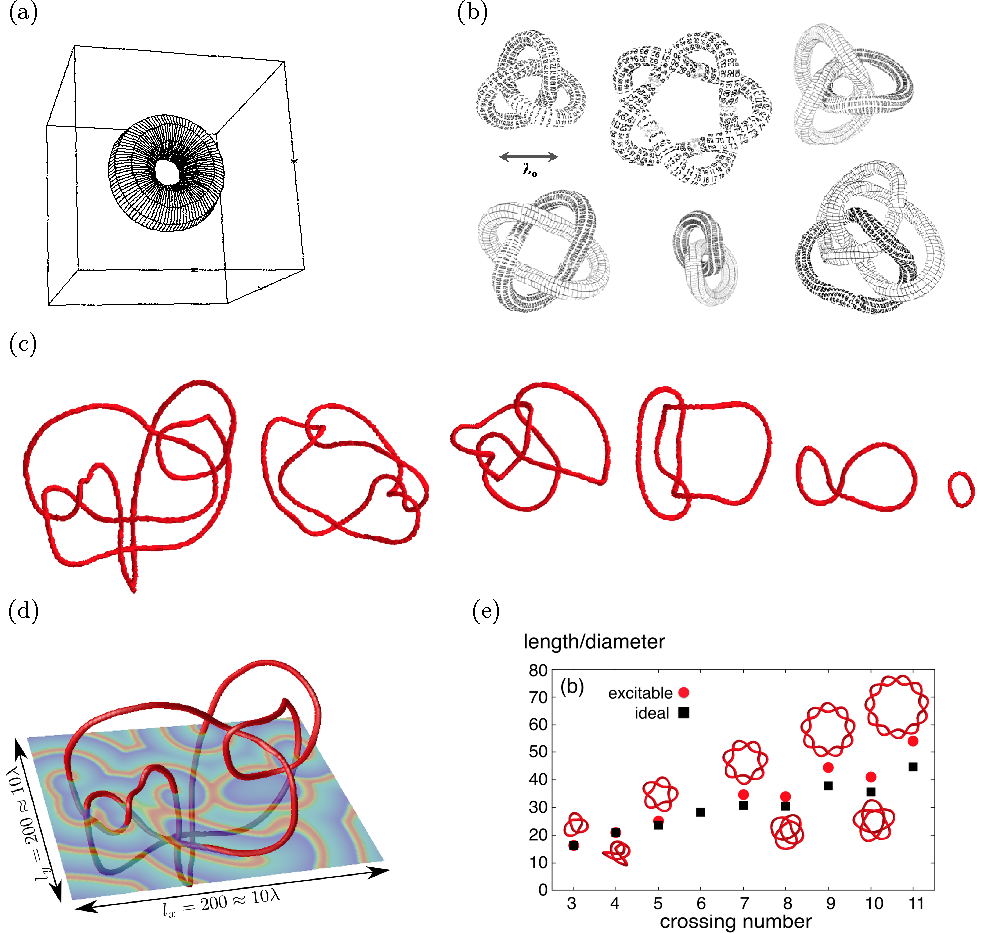
\includegraphics[width=\linewidth]{\IntroductionFigures/FNKnots.pdf}
\caption{Stable knotted vortices in the FitzHugh-Nagumo model. (a) A vortex ring contracts to a stable radius and drifts at constant velocity; its radius is 0.23$\lambda_0$, where $\lambda_0$ is the wavelength of the spiral wave in the medium (see scale bar in panel (b)) . (b) An assortment of apparently stable knotted and linked vortices found in Ref.~\citep{Henze1993}. The tube around the knots is of diameter $\lambda_0/\pi$. The stability of the trefoil knot and Hopf link were subsequently confirmed in Ref.~\citep{Sutcliffe2003} (the others are, in fact, unstable in the bulk). (c,d) The FitzHugh-Nagumo dynamics are capable of simplifying a tangled, but unknotted, curve to the canonical round form of panel (a); panel (c) shows an example simplification, with a cross section through the vortex knot in panel (d) showing the wavefield.(e) Recently, stable forms for torus knots and the figure-eight knot were found. Their geometries are shown here, alongside their lengths as compared to ideal ropelengths. Figures reproduced from Ref.~\citep{Winfree1990,WinfreeChapter,Maucher2016,Maucher2017}.}
\label{fig:FNKnots}
\end{figure}
These numerical findings are in stark contrast to what we saw in fluids, superfluids and liquid crystals (indeed, in most knotted fields), and invite a series of questions: What determines the dynamics of these vortices? How are reconnections avoided? What is the mechanism of knot untangling? Are all knots stable, and if so can we predict their shapes? In some form these questions have existed since the first knotted vortices were discovered. Initial theoretical work focused heavily on the idea that their laws of motion could be explained by a `local geometry hypothesis'~\citep{Keener1988,Keener1992,Biktashev1994,Henry2002,Echebarria2006,Dierckx2010} in which dynamics at each point on the curve were governed by some local law of motion involving its curvature, the twist of spiral wave phase etc. After a perturbative theory for such a law was developed~\citep{Keener1988,Keener1992, Biktashev1994}, substantial work went into testing whether or not this was the case~\citep{Winfree1990,Henze1993}, of which an account may be found in \citep{WinfreeChapter}. Summarising very coarsely, such laws found some success in describing isolated filaments, but of course encounter problems whenever interfilament interactions are required. The problem is that evidence ultimately suggested such interactions were integral to describing stable knots \citep{Henze1993,WinfreeChapter}, and as such a local geometry hypothesis failed to account for their dynamics. The observed untangling without reconnection of unknots shown in figure~\ref{fig:FNKnots}(e) \citep{Maucher2016} further casts doubt on whether such a law could be made to work. 

We remark that the idea of reducing the dynamics of an entire field to that of a curve is not unique to excitable media, but cuts across knotted fields. In particular the idea is similar to the Local Induction Approximation (LIA) in fluids and superfluids \citep{Saffman1992}, in which the Biot-Savart law of motion governing vortex lines is approximated by a dominant contribution arising from local curvature, which leads to motion binormal to the curve --- in the case of a vortex ring, drift perpendicular to the plane it lies in, a feature shared by the rings studied here \citep{Winfree1990}. Further, exact knotted solutions to the LIA \emph{do} exist \citep{Hasimoto1972,Kida1981}, and one might have hoped something similar applied here. Note however that the LIA breaks down in fluids too, and further that the nature of the fields surrounding the vortices is quite different between the two cases. One crucial difference, as we shall see, is that in excitable media waves propagate without attenuation for potentially arbitrary distances, making a theoretical decoupling of distant segments of the knot difficult. 

In summary, the questions posed above are not satisfactorily answered. Our attempts to explore them, with a focus on systematically testing knots for stability and exploring the importance of nonlocal filament interactions, form \S \ref{ch:FitzHughNagumo}. The potential for experimentally accessible, and spontaneously stable, knotted fields is a major motivator for this work.

\section{This thesis}

This thesis is primarily about knotted fields in soft matter systems, systems that may be loosely characterised as those in which geometry plays a fundamental role, and which may undergo substantial deformations in response to external forces, changes in temperature etc. All three of the systems described above might be considered examples of soft matter systems. One might ask ``why choose soft matter?'' and we hope that our descriptions of the experimental possibilities of such systems provide an immediate answer. Their combination of rich geometric structure and experimental accessibility make them natural testbeds for exploring knotted fields in all their guises. In our focus on soft matter we have of course been selective, completely neglecting discussion of theoretical and computational advances in optics \citep{Bode2017,Dennis2017}, electromagnetism \citep{Ranada1989, Ranada1990, Ranada1992,Irvine2010,Kedia2013,Kedia2016,Arrayas2017,Kedia2018} and high energy physics \citep{Faddeev1997, Houghton1998,Battye1998,Battye1999, Sutcliffe2007}. Even within the realm of soft matter we have been selective; fluids stand out as the first and most highly developed examples of knotted fields, and as such it was natural to discuss them. Beyond that, as well as important examples of knotted fields in their own right, our presentation of material on liquid crystals and excitable media serve as background and motivation for the research topics addressed in this thesis.

As for the research topics themselves, they fall under the broad heading of `investigations into knotted fields in soft matter', but each is a distinct story. Primarily they were chosen simply in response to current interesting questions in knotted fields. As for \S\ref{ch:FitzHughNagumo}, Maucher and Sutcliffe's paper on unknot simplification \citep{Maucher2016} was published in 2016, and one might take it as marking renewed interest in questions around the FitzHugh-Nagumo model --- there is a gap of $13$ years between it and the last publication on the matter \citep{Sutcliffe2003}. Coupled with improved computational abilities\footnote{Compare the description in Ref.~\citep{Henze1993} of running code on a CRAY supercomputer to my own experience on my laptop and the Warwick cluster.}, new ideas about knot initialisation, and the recent experiments we discussed in \S \ref{sec:FN}, it seems a natural time for new investigation. \S\ref{ch:TwistBend} is again a development of recent questions about the geometry and topology of liquid crystal gradients; our focus will be on the topology of bend distortions. As we have seen, more theoretical attention has been paid to orthogonal gradients and twist \citep{Bellar2014,Machon2016, Machon2017} than to bend (however there is recent work on splay and bend in two dimensions \citep{Niv2018}) and it is natural to try and complete the picture. The recent discovery of twist-bend and splay-bend nematic phases, of which the first review was published in 2018 \citep{Lavrentovich2018}, provides further motivation as a natural experimental setting for theoretical constructs, a role the cholesteric plays for twist. The content of \S \ref{ch:Maxwell}, on theoretical constructions for initialising knotted vortices, is a little different: it initially arose out of a practical need to do just that in \S\ref{ch:FitzHughNagumo}. Many other methods exist and will be discussed in \S\ref{ch:Maxwell}, but in one way or another they did not suit our needs, either because the geometries of knot they allowed were restricted, or they were computationally problematic. In attempting to solve this practical problem, we were led to re-evaluate Maxwell's work on the solid angle function \citep{Maxwell2}, extending it to knots and discovering connections between the various different methods he proposes for constructing the function, as well as connections to modern work on curve framings, writhe etc. As a result, this chapter has a `half theoretical, half practical' feel. Its content was subsequently used in the simulations presented in \S\ref{ch:FitzHughNagumo} and in constructing the self-linkings of bend zeros described in \S\ref{ch:TwistBend}.

We now provide a more technical summary of the content of each chapter, with reference to the foregoing discussion.

\subsubsection{\S \ref{ch:Maxwell}: Maxwell's Theory of Solid Angle and the Construction of Knotted Fields}

This chapter addresses a question which cuts across particular systems, and has not been much discussed above: Theoretically, how should one construct a knotted field? In order to simulate a knotted superfluid vortex (figure~\ref{fig:SuperFluidMontage}), a knotted vortex in the FitzHugh-Nagumo model (figure~\ref{fig:FNKnots}), or any other knotted system one needs a method of initialising a topologically correct configuration before running dynamics. For the above examples, this amounts to constructing a phase field $\phi \in S^1$ containing a phase singularity with the topology (and possibly geometry) of the desired knot. 

In this chapter we propose the solid angle function of a link $K$, defined by Maxwell in his \emph{A Treatise on Electricity and Magnetism} \citep{Maxwell2}, as a natural solution to this problem. We provide a systematic description of this function as a means of constructing a knotted field for any curve or link in $\mathbb{R}^3$. This is a purely geometric construction in which all of the properties of the entire knotted field derive from the geometry of the curve, and from projective and spherical geometry. We emphasise a fundamental homotopy formula as unifying different formulae for computing the solid angle. The solid angle induces a natural framing of the curve, which we show is related to its writhe $Wr$ and use to characterise the local structure in a neighbourhood of the knot. Finally, we discuss computational implementation of the formulae derived, and give illustrations for how the solid angle may be used to give explicit constructions of knotted vortices in excitable media and knotted director fields around disclination lines in nematic liquid crystals. Part of the work in this chapter consists of an implementation of the methods described in C++: it may be found at \href{https://github.com/garethalexander/SolidAngle}{https://github.com/garethalexander/SolidAngle}.

TODO:INCLUDE IN THE APPENDIX

\subsubsection{\S \ref{ch:TwistBend}: Bend Geometry in Liquid Crystals}
TODO: FILL THIS IN

\subsubsection{\S \ref{ch:FitzHughNagumo}: Stable and Unstable Vortices in Excitable Media}
In \S \ref{sec:FN} we discussed the discovery of several apparently stable knotted vortices in the FitzHugh-Nagumo model, as well as the dynamics' remarkable ability to simplify unknots without reconnections. We also saw that the mechanisms underlying these phenomena are still ill-understood, and posed the following questions: What determines the dynamics of these vortices? How are reconnections avoided? What is the mechanism of knot untangling? Are all knots stable, and if so can we predict their shapes? This chapter is an exploration of these questions. We perform a systematic survey of the dynamics of all knots with at most eight crossings, establishing that the generic behaviour is of unsteady, irregular dynamics, with prolonged periods of expansion of parts of the vortex. We show that the mechanism for the length expansion is a long-range “wave-slapping” interaction. We also show that there are stable vortex geometries for certain knots; in addition to the unknot, trefoil, and figure-eight knots reported previously, we have found stable examples of the Whitehead link and $6_2$ knot. We give a thorough characterisation of their geometry and steady-state motion. For the unknot, trefoil, and figure-eight knots we greatly expand previous evidence that FitzHugh-Nagumo dynamics untangles initially complex geometries while preserving topology, and discuss the mechanisms at play.







     \chapter{Maxwell's Theory of Solid Angle and the Construction of Knotted Fields}
    \label{ch:Maxwell}
    \section{Introduction}

    Knotted fields are three-dimensional textures of continuous media that encode in their structure a knotted curve, filament or family of field lines. Originating in Lord Kelvin's speculations of atomic structure as knotted vortices in the aether~\citep{Kelvin}, they have since been experimentally realised in nodal lines of optical beams~\citep{Dennis2010}, disclinations in nematic liquid crystals~\citep{Tkalec2011,Tasinkevych2014,Copar2015}, spinor Bose-Einstein condensates and fluid vortices~\citep{Kleckner2013}. Concurrently, theoretical studies continue to flourish in classical field theory~\citep{Sutcliffe2007}, electromagnetism~\citep{Kedia2013,Arrayas2017}, superfluids \citep{Kleckner2016} and excitable media~\citep{Maucher2016,Maucher2017,Maucher2018}.

    Central to theoretical advances are explicit constructions for knotted fields exhibiting different knot types, or other pertinent physical properties, such as helicity in fluid flows. Constructions for knots in electromagnetic fields have centred around the Hopf map and rational map generalisations of it, shear-free null congruences and twistor methods~\citep{Ranada1992,Kedia2013,Arrayas2017,Kedia2018}. The simplest constructions yield torus knots and links and the majority of constructions have focused on this family, together with seeking to control the helicity of the field~\citep{Kedia2018}, or its dynamics~\citep{Irvine2010}. The same rational map constructions also give knotted solutions in other field theories, such as the Skyrme-Faddeev model~\citep{Battye1998,Sutcliffe2007}. These methods satisfy the dynamical equations of motion directly and are geometrically special by construction, providing powerful tools for describing the full knotted field and its properties. 

    A separate approach has been developed to create nodal lines in optical beams that encodes the knot as the zero locus of a complex polynomial~\citep{Dennis2010}. From these fields initial conditions can be generated for paraxial wave equations with the subsequent evolution giving a beam containing the encoded knot. Again, the simplest constructions are for torus knots (captured by the polynomials $z_1^p+z_2^q$) but the method can be applied for any geometric braid~\citep{Bode2017,Dennis2017}. The argument of such a complex polynomial gives a phase field that winds around the knotted nodal line and can be used to initialise phase vortices, or as an angle orienting the director field of a liquid crystal with the nodal line then appearing as a disclination~\citep{Machon2014}. In common with the constructions for electromagnetic knots, this approach encodes the knot implicitly rather than explicitly in that its location and geometry derives from the polynomial rather than being given {\sl a priori}. 

    A canonical construction for a phase field associated to any knotted curve $K$, that depends only on the curve and represents a knotted field on its complement is given by the solid angle $\omega(\bf{x})$ subtended by $K$ at each point in space. This construction of knotted fields goes back to Maxwell~\citep{Maxwell2}, since the solid angle is proportional to the magnetostatic potential of a current carrying wire, and in all likelihood represents the earliest explicit construction for a knotted field. 
    If we imagine $K$ to be a wire carrying unit current then Maxwell's equations state that it generates, in its complement, a magnetic field that is irrotational, so that locally it is the gradient of a potential. Amp\`ere's law shows this potential to be globally multi-valued (increasing by $\mu_0$ upon traversing any closed loop encircling the wire): the solid angle is the magnetostatic potential normalised to be $4\pi$ cyclic, {\sl i.e.} it takes values in $\mathbb{R}/4\pi\mathbb{Z}\cong S^1$. This description makes clear that solid angle is naturally defined for an oriented curve $K$, the orientation being provided by the current flow. Since magnetic fields are divergence free, the solid angle is a harmonic function, and this, together with the $4\pi$ circulation, may be taken as an alternative definition. Knotted fields constructed out of it satisfy physical differential equations (Laplace's equation), but in contrast to other methods are more direct and explicit in their construction, so that there is no special focus on torus knots, geometric braids or any other particular class of knots. 

    Construction of the magnetostatic potential via numerical integration of the magnetic field about $K$ has recently been used to initialise knotted fields in superfluids and excitable media~\citep{Kleckner2016,Maucher2016}. However, very little in the way of a systematic treatment of solid angle and its geometric content has been given since Maxwell's own presentation in his {\sl Treatise on Electricity and Magnetism}~\citep{Maxwell2}. Maxwell devotes articles~417-422 of Ref.~\citep{Maxwell2} to an extended discussion of solid angle, its properties and geometric meaning, as well as methods for calculating it. He gives three methods, in addition to~\eqref{eq:SolidAngle1}: a direct calculation; a method given ``for the sake of geometrical propriety''; and his preferred method which involves calculating the work done in transporting a unit magnetic pole to the point ${\bf x}$. Through the latter he (independently) derives the Gauss linking integral~\citep{Ricca2011}. 

    Typically, solid angle is described with the help of an orientable surface $\Sigma$ spanning $K$: $\omega({\bf x})$ is then the area that this surface projects to on the unit sphere centred on $\bf x$, and is given explicitly by the formula~\citep{Saffman1992} (which Maxwell attributes to Gauss~\citep[Art.~409]{Maxwell2})
    \begin{equation}
        \omega({\bf x}) = \int_{\Sigma} \frac{({\bf x}-{\bf y})}{|{\bf x}-{\bf y}|^3}\cdot \mathrm{d}{\bf S} ,
        \label{eq:SolidAngle1}
    \end{equation}
    where ${\bf y}$ varies over $\Sigma$. While this description hides the fact that solid angle depends only on $K$, it provides the main geometric interpretation for solid angle and establishes close connections to projective and spherical geometry, particularly to spherical curves and areas. Solid angle, then, is a naturally geometric object dependent only on $K$, which involves an interplay between the geometry of $K$ itself, and that of the spherical curve to which $K$ projects. As such it belongs firmly to the domain of the differential geometry of curves. Yet its relationship to curve geometry is only partially developed, limited to how the local geometry influences the local structure of the magnetic field in the curve's normal plane~\citep{Saffman1992,Moore1972,Ricca1994}. A related question is that of an `optimal' method of computing $\omega$, both from a theoretical and computational standpoint. Both methods mentioned above suffer deficiencies. In the first, an unnecessary intermediate, the magnetic field, is computed before $\omega$. In the second, an arbitrary surface spanning $K$ must be provided, of which $\omega$ is independent --- this is especially inconvenient from a numerical standpoint. We desire a convenient direct expression for $\omega$, dependent only on $K$. 

    In this chapter, we show that Maxwell's three methods, extended where appropriate to knotted curves, may all be considered as applications of a single curve homotopy formula. In doing so, we shall arrive at several distinct formulae for computing $\omega$ directly from $K$ and make connections between solid angle and modern results on the geometry of spherical curves~\citep{Levi1994,Arnold1995}, as well as discussing close connections between the asymptotic structure of $\omega$ and the writhe of $K$~\citep{Fuller1978,Dennis2005}. With these formulae in place, we offer a geometric description of the local properties of $\omega$ in a tubular neighbourhood of $K$, considering both the structure in the normal plane and as one moves along the knot. Our description, which begins directly at the spherical geometry of the projected curve, complements existing results on the local structure of the magnetic field, and reveals a previously unseen connection between the local structure of $\omega$ and the `writhe framing' of Ref.~\citep{Dennis2005}. 
    Our results give several formulae for the direct computation of $\omega$ from $K$, of practical value when initialising simulations of knotted fields. We discuss solutions to the main difficulties in their numerical implementation, and end with a brief description of applications to the initialisation of scroll waves in excitable media and knotted textures in nematics. Implementations in C of the methods described are given at \verb=github.com/garethalexander=.

    The extension of the construction of solid angle to the case where $K$ is a link is straightforward: by the linearity of electromagnetism the solid angle for a link is simply the sum (mod $4\pi$) of the solid angles corresponding to each of the link components. For this reason, we restrict the majority of our discussion to knots, and discuss the few subtleties which come with extension to links in a brief dedicated section.

    \section{The homotopy formula for solid angle} 
    \label{sec:CurveIsotopies}

    \begin{figure}[t]
        \centering	
        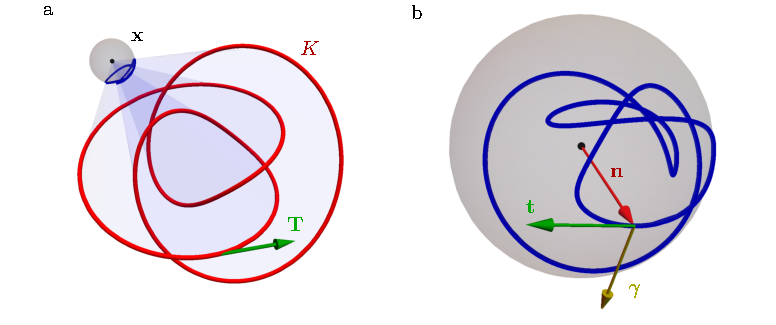
\includegraphics[width=\textwidth]{\MaxwellFigures/Figure1.pdf}
        \caption[Spherical knot projection onto an observation point.]{(a) An oriented knot $K$ with tangent vector $\bf T$ (here the $4_1$) projects onto a unit observation sphere about a point $\bf x$, giving the spherical curve shown in blue. (b) The projection of $K$ onto the observation sphere gives an immersed spherical curve $\bf n$, with self-intersections in correspondence with the crossings of the knot as seen from $\bf x$. A unit tangent $\bf t$ for $\bf n$ is induced by the orientation of $K$, and we select normal $\boldsymbol{\gamma} := \bf n \times \bf t$.}
        \label{fig:Knot} 
    \end{figure}

    At each point ${\bf x}$ of the knot complement the projection of $K$ onto the unit sphere centred on ${\bf x}$, which we shall call the observation sphere, traces out a curve ${\bf n}:=\frac{{\bf y}-{\bf x}}{|{\bf y}-{\bf x}|}$, ${\bf y}\in K$, as shown in figure~\ref{fig:Knot}. This projected curve has points of self-intersection in correspondence with the crossings of the knot as seen from ${\bf x}$. Upon varying ${\bf x}$ there will be particular viewing points where the number of visible crossings changes and at those points ${\bf n}$ also has cusps. In all cases~\eqref{eq:SolidAngle1} expresses that the solid angle at ${\bf x}$ is the area bound by the projected curve ${\bf n}$ on the observation sphere; indeed, Maxwell states this as the definition of the solid angle. 

    Maxwell's first method of computing $\omega({\bf x})$ is to choose arbitrary spherical coordinates $(\theta,\phi)$ on the observation sphere, and integrate the projected area directly~\citep[Art.~417]{Maxwell2}:
    \begin{equation}
        \omega({\bf x}) = \int (1 - \cos \theta)~\mathrm{d}\phi .
        \label{eq:MaxSphere}
    \end{equation}
    If we denote by ${\bf n}_{\infty}$ the (arbitrarily chosen) polar direction $\theta=0$, then~\eqref{eq:MaxSphere} can be expressed in vector notation as 
    \begin{equation}
        \omega({\bf x}) = \int \frac{{\bf n}_{\infty} \times {\bf n} }{1+{\bf n}_\infty \cdot {\bf n}} \cdot \mathrm{d}{\bf n} ,
        \label{eq:OurSolidAngle1}
    \end{equation}
    a formula that has been rediscovered a number of times~\citep{Asvestas1985,Dangskul2015,Borodzik2017}. We remark that if we interpret~\eqref{eq:OurSolidAngle1} as an integral over $K$ rather than its projection on the observation sphere, the integrand is the vector potential for a magnetic monopole placed at ${\bf x}$, with $-{\bf n}_{\infty}$ corresponding to the choice of Dirac string. Indeed, expressing it in the spherical coordinates of~\eqref{eq:MaxSphere} we recover the vector potential of Ref.~\citep{Dirac1931}
    \begin{equation}
        \frac{{\bf n}_{\infty} \times {\bf n} }{1+{\bf n}_\infty \cdot {\bf n}} \cdot \frac{1}{| \bf {y - x} |} = \frac{\sin{\theta}}{r(1+\cos{\theta})}\boldsymbol{\hat{\phi}}, 
    \end{equation}
    where $r = |{\bf y -x}|$. Maxwell gives this formula explicitly in Cartesian coordinates and remarks on the role of the string (``axis'') in evaluating the integral. 

    Maxwell does not advocate the use of~\eqref{eq:MaxSphere}, other than for computational convenience, writing that it ``involves a choice of axes which is to some extent arbitrary, and it does not depend solely on the closed curve''~\citep[Art.~418]{Maxwell2}. We shall discuss his second method in \S\ref{sec:GaussBonnet}, but his preferred method is his third ``as it employs no constructions which do not flow from the physical data of the problem''~\citep[Art.~419]{Maxwell2}: viewing $\omega$ as the magnetostatic potential of $K$, it may be built by measuring the change $\Delta\omega$ as we transport a unit magnetic pole along an arbitrary path from a reference location to ${\bf x}$, or equivalently by fixing ${\bf x}$ and oppositely transporting $K$. Maxwell gives a formula for $\Delta\omega$ under this transport in terms of a double integral over the path and $K$, by summing the areas of the infinitesimal parallelograms swept out by line elements of $K$. 

    This approach shifts the focus from calculating the solid angle directly to calculating the change induced by a translation of the knot along some path. It is a small step to extend this to give a formula for the change associated to a general homotopy of $K$, in which the shape of $K$ may vary. Of course, $\Delta \omega$ does not depend on the precise form of this homotopy, which allows it to be calculated using a standardised method, for instance by connecting corresponding points of the initial ($K_0$) and final ($K_1$) curves with straight lines, {\sl i.e.} $K_t = (1-t) K_0 + t K_1$, $t\in [0,1]$. This homotopy induces one on the observation sphere, which we denote ${\bf n}_t$, with the straight lines along which the points of $K$ move projecting to geodesic arcs connecting ${\bf n}_0$ and ${\bf n}_1$. The change in solid angle is the area swept out by this mesh of geodesic arcs. 

    Consider the contribution to the area of the geodesics connecting a small segment of the two curves: By Archimedes' theorem on the equality of the area of the sphere and its circumscribed cylinder this is equal to the product of the distance $|{\bf n}_0-{\bf n}_1|$ between the two endpoints of the geodesic arc and the angle swept out by its midpoint $({\bf n}_0+{\bf n}_1)/|{\bf n}_0+{\bf n}_1|$. The difference in solid angle is therefore 
    \begin{align}
        \omega({\bf x}; K_1) - \omega({\bf x}; K_0)
        &=
        \int ({\bf n}_0 - {\bf n}_1) \times \frac{{\bf n}_0 + {\bf n}_1}{|{\bf n}_0 + {\bf n}_1|} \cdot \mathrm{d} \frac{{\bf n}_0 + {\bf n}_1}{|{\bf n}_0 + {\bf n}_1|} \quad  \nonumber \\ 
        &=
        \int \frac{{\bf n}_0 \times {\bf n}_1 \cdot ( \mathrm{d}{\bf n}_0 + \mathrm{d}{\bf n}_1 )}{1+{\bf n}_0 \cdot {\bf n}_1} \quad \textrm{mod } 4\pi.
        \label{eq:Isotopy}
    \end{align}
    This is the basic homotopy formula for solid angle, applicable to an arbitrary deformation of $K$. Both Maxwell's first and third methods of computing $\omega$ can be seen as applications of~\eqref{eq:Isotopy} --- we recover~\eqref{eq:OurSolidAngle1} by letting $K_0$ recede asymptotically far from $\bf x$, so that ${\bf n}_0$ is a single point ${\bf n}_{\infty}$ on the observation sphere and $\omega({\bf x}; K_0)=0$ mod $4\pi$. In \S\ref{sec:GaussBonnet} we shall use a homotopy of $K$ along its tangent developable surface to demonstrate that his second method also follows directly from the homotopy formula. 

    The integral in~\eqref{eq:Isotopy} is not defined when $\bf x$ lies on the surface swept out by $K_t$, which we refer to as the surface of discontinuity --- as an example, in~\eqref{eq:OurSolidAngle1} this surface is formed by translating $K$ to infinity along ${\bf n}_\infty$. The line of $K_t$ passing through $\bf x$ connects antipodal points of the observation sphere, ${\bf n}_0 \cdot {\bf n}_1= -1$, and this line does not project to a unique geodesic arc connecting these endpoints. Instead there is a whole family of equivalent connecting geodesics, which cover the sphere once. As $\bf x$ crosses the surface of discontinuity, the geodesic parameterisation of the antipodal sections of ${\bf n}_0$ and ${\bf n}_1$ jumps from one side of the observation sphere to the other, giving a $4 \pi$ jump in~\eqref{eq:Isotopy}.

    We note that~\eqref{eq:Isotopy} has the same form as the formula given by Fuller for the difference in writhe of two curves~\citep{Fuller1978}. This is because for each fixed point ${\bf x}$ (not on $K_t$ for any $t$) the difference in solid angle is expressible as an area between two spherical curves, as arises for the difference in writhe. This is the first of several relations between the solid angle function for a curve and its writhe, which help to convey its geometric content.

    \section{Maxwell's geometric formula, dual curves and homotopies along tangent developable surfaces }
    \label{sec:GaussBonnet}
    \begin{figure}
        \centering
        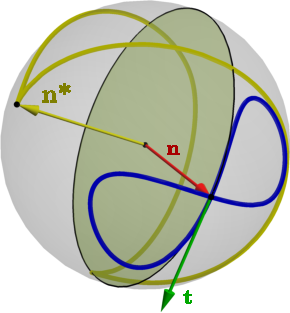
\includegraphics{\MaxwellFigures/Figure9.pdf}
        \caption[The dual curve construction.]{A spherical knot projection $\bf n$ (blue curve, here a typical projection of a twisted unknot) induces a dual spherical curve ${\bf n}^* := {\bf t} \times {\bf n}$ (yellow curve). Maxwell proposes the construction of ${\bf n}^*$ by allowing a unit circle (yellow disk) to roll without slipping around $\bf n$ such that its plane of contact is tangent to $\bf n$. A unit vector perpendicular to this circle (yellow arrow) then traces ${\bf n}^*$. As shown in~\eqref{eq:dn*ds}, zeros of geodesic curvature in $\bf n$ correspond to cusps in $\bf n^*$ (marked points). More pictures of this construction may be found in Refs. \citep{Levi1994,Arnold1995}.   }
        \label{fig:DualCurve} 
    \end{figure}
    Maxwell's objection to~\eqref{eq:MaxSphere} is that it involves an arbitrary choice of spherical coordinates on the observation sphere, and for this reason he states a construction in which no such choice is made \citep[Art.~418]{Maxwell2}. Let a unit circle roll without slipping around ${\bf n}$ such that its plane of contact is tangent to $\bf n$, as shown in figure~\ref{fig:DualCurve}. Then a unit vector perpendicular to this circle traces a second curve on the observation sphere, called the dual curve ${\bf n}^*$. Denote the length of ${\bf n}^*$ by $\sigma$. Maxwell states that the solid angle is given by 
    \begin{equation}
        \omega({\bf x}) = 2\pi - \sigma ,
        \label{eq:DualCurve}
    \end{equation}
    a result he simply describes as a ``well-known theorem''. This result is in fact equivalent to the Gauss-Bonnet formula~\citep{Lee1996}, an identification that has been rediscovered at least twice~\citep{Levi1994,Arnold1995}. In the form stated by Maxwell,~\eqref{eq:DualCurve} is only correct if ${\bf n}$ is a simple curve without points of inflection, but it is true in much greater generality~\citep{Arnold1995}. As a more general version is essential for application to generic knot projections, we give a self-contained elementary proof, applicable to any smoothly immersed spherical curve. 

    \subsection{A dual curve theorem for self-intersecting curves}
    \label{subsec:GaussBonnetSelfIntersecting}
    \begin{figure}
        \centering
        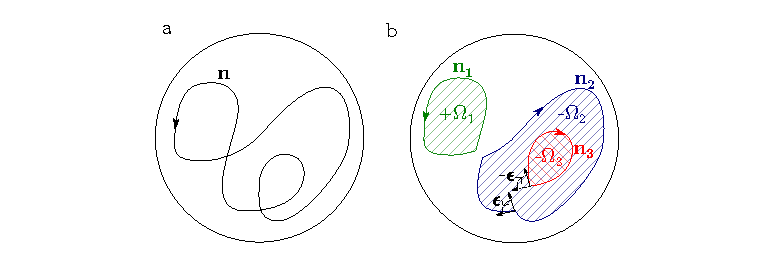
\includegraphics[width=\textwidth]{\MaxwellFigures/Figure2.pdf}
        \caption[Decomposition of the spherical knot projection.]{The spherical knot projection $\bf n$ in panel (a) may be decomposed via the Seifert algorithm into Seifert circles ${\bf n}_i$, shown in panel (b). These circles bound regions $\Omega_i$, signed according to the orientation of their boundary (coloured hatching). At self-intersection points of $\bf n$, the resulting circles have corners, with exterior angles $\epsilon_{ij}$ (shown for one such corner).}
        \label{fig:GaussBonnet} 
    \end{figure}

    We begin by relating the area swept out by ${\bf n}$ to its integrated geodesic curvature by using the Gauss-Bonnet formula. ${\bf n}$ has a canonical tangent vector induced from the orientation of $K$, denoted $\bf t$, and we choose for it a normal vector $\boldsymbol \gamma := \bf n \times \bf t$, as shown in figure~\ref{fig:Knot}(b). (Note that in the special case that ${\bf n}$ is a simple curve it bounds two regions on the sphere, but is only correctly oriented as the boundary of one of them. ${\boldsymbol \gamma}$ points inwards to this region.) We perform a Seifert decomposition~\citep{Adams2004} of ${\bf n}$. This entails resolving each crossing in a manner that preserves the orientation of the curve and results in its separation into a collection of Seifert circles ${\bf n}_i$, as shown in figure~\ref{fig:GaussBonnet}. Each circle is a simple curve and bounds a region $\Omega_i$. At self-intersections of ${\bf n}$ the Seifert circles have corners, with exterior angles $\epsilon_{ij}$. Now, for each circle, the Gauss-Bonnet formula tells us
    \begin{equation}
        \int_{\Omega_i} \mathrm{d} A  = 2 \pi - \int_{{\bf n}_i} k_{\boldsymbol \gamma} \mathrm{d} s - \sum_j \epsilon_{ij} ,
        \label{eq:GaussBonnetSeifert}
    \end{equation}
    where $k_{\boldsymbol \gamma} = \frac{d {\bf t}}{d s} \cdot {\boldsymbol \gamma}$ is the signed geodesic curvature of the boundary. Summing over all Seifert circles, the left-hand-side gives $\omega({\bf x})$ mod $4\pi$; on the right-hand-side the exterior angles cancel pairwise, and we pick up a contribution of $2\pi S$, where $S$ is the number of Seifert circles, in addition to the total integrated (signed) geodesic curvature. The number of Seifert circles is equal to $\chi + D$, where $\chi$ is the Euler characteristic of the surface constructed by the Seifert algorithm and $D$ is the number of double points (self-intersections)~\citep{Adams2004,Lickorish1997}. For a knot the Euler characteristic of any Seifert surface is odd, so that $S = D+1$ mod $2$. Thus we have
    \begin{equation}
        \omega({\bf x})  = 2 \pi (D + 1) - \int_{{\bf n}} k_{\boldsymbol \gamma} \mathrm{d}s\quad\textrm{mod}\; 4\pi .
        \label{eq:GaussBonnetImmersed}
    \end{equation} 
    We remark that the quantity $D+1$ mod $2$ is the spherical equivalent of the rotation number of a planar self-intersecting curve, sometimes termed its parity \citep{Whitney1937,Phillips1966,Solomon1996}. The $2 \pi$ in the Gauss-Bonnet formula arises as the rotation number of a simple curve, and the appearance of the parity here is thus a natural extension to the self-intersecting case. 

    The integrated geodesic curvature is equal to the (signed) length of the dual curve ${\bf n}^* := -{\boldsymbol \gamma} = {\bf t} \times {\bf n}$ \citep{Levi1994,Arnold1995}(figure~\ref{fig:DualCurve}). To see this, consider how ${\bf n}^*$ varies with arc length along ${\bf n}$:
    \begin{equation}
        \frac{\mathrm{d}{\bf n}^*}{\mathrm{d}s} = \frac{\mathrm{d}\,}{\mathrm{d}s}({\bf t} \times {\bf n}) = \frac{\mathrm{d}{\bf t}}{\mathrm{d}s} \times {\bf n}= k_{{\boldsymbol \gamma}} {\bf t} .
        \label{eq:dn*ds}
    \end{equation}
    ${\bf t}$ is tangent to ${\bf n}^*$, but its orientation alternates across zeros of $k_{\boldsymbol \gamma}$, which correspond to cusps in ${\bf n}^*$. Defining $ds^* = k_{\boldsymbol \gamma}ds$, we obtain $\mathrm{d}{\bf n}^*/\mathrm{d}s^* = {\bf t}$, and see that $ds^*$ should be interpreted as a signed length element, the sign being given by that of $k_{\boldsymbol \gamma}$. Thus we arrive at
    \begin{equation}
        \omega({\bf x}) =  2 \pi (D+1) - \int_{{\bf n}^*} \mathrm{d} s^* \quad \mathrm{mod}\; 4\pi . 
        \label{eq:DualCurveImmersed}
    \end{equation}
    For a simple curve without inflection points $D=0$ and the sign of $\mathrm{d}s^*$ never alternates, so its integral gives $\sigma$ and we recover~\eqref{eq:DualCurve}. By contrast, consider the spherical `figure-eight' curve $\bf {n}$ shown in figure~\ref{fig:DualCurve}, as would arise when $K$ is a twisted unknot parameterised by $(\sin t, \cos t, \sin 2t), t\in [0,2\pi]$, and the point of projection lies on the $y$-axis with $|y|>1$. Considering a surface spanning this twisted unknot, one immeadiately expects $\omega=0$ at such a projection point --- let us check the results of \eqref{eq:DualCurve}, \eqref{eq:DualCurveImmersed} applied to the spherical figure-eight curve. $D=1$ and we have two zeros of geodesic curvature, which divide $\bf{n}^*$ into two segments separated by cusps with $ds^*$ switching sign between them. So applying~\eqref{eq:DualCurveImmersed}, we arrive at our expected result, but applying~\eqref{eq:DualCurve} we do not. Eq.~\eqref{eq:DualCurveImmersed} thus generalises Maxwell's ``well known theorem''~\eqref{eq:DualCurve} to the case of a smoothly immersed curve, and in particular to any generic spherical knot projection. 

    \subsection{The pullback to $K$ and a homotopy along the tangent developable surface}
    \label{subsec:Pullback}

    As a result on the structure of spherical areas,~\eqref{eq:DualCurveImmersed} is valid for any smoothly immersed spherical curve. However, we have in mind the case where one arises as the projection of the knot $K$. Using this projection we now pull each term in~\eqref{eq:DualCurveImmersed} back to $K$. This facilitates a reinterpretation in terms of the geometry of $K$, as well as a novel method of deriving it using~\eqref{eq:Isotopy}.

    We begin by constructing a natural `projective' framing for $K$, dependent on $\bf x$, with which we will express $D$ in~\eqref{eq:DualCurveImmersed} as a self-linking number. To construct this framing, extend the lines of sight from ${\bf x}$ along ${\bf n}$ until they meet $K$. These lines project to vectors normal to $K$, which are non-zero provided ${\bf n} \cdot {\bf T} \neq \pm 1$ where ${\bf T}$ is the unit tangent vector to $K$, in other words provided there are no cusps in ${\bf n}$ on the observation sphere. The number of double points seen from $\bf x$ mod $2$ is equal to the self-linking number of $K$ given this projective framing, $\mathrm{SL}(K,{\bf x})$, also mod $2$. The mod $2$ counting gives an ambiguity in the sign of the identification of $D$ with $\mathrm{SL}(K,{\bf x})$ which will lead to two distinct re-writings of~\eqref{eq:DualCurveImmersed}, and so we shall keep the sign explicit in the following. 

    Using C\u{a}lug\u{a}reanu's theorem~\citep{Calugareanu1959,Calugareanu1961}, $ \mathrm{SL}(K,{\bf x}) = \mathrm{Tw}(K,{\bf x}) +\mathrm{Wr}(K)$, we now write $ \mathrm{SL}(K,{\bf x})$ in terms of the writhe of $K$ and the twist of the projective framing, which is directly computed to be 
    \begin{equation}
        \mathrm{Tw}(K,{\bf x}) = \int_K  \frac{ ( {\bf n} \cdot {\bf T} ) ({\bf n} \cdot {\bf T} \times \mathrm{d}{\bf T}) }{1 - ({\bf n} \cdot {\bf T})^2} . 
        \label{eq:Twist}
    \end{equation}
    Substituting this expression for $\mathrm{SL}(K,{\bf x})$ into~\eqref{eq:DualCurveImmersed} with the sign ambiguity discussed above, and combining with the pullback of the dual curve length,
    \begin{equation}
        \int_{{\bf n ^*}} \mathrm{d} s^* = \int_{{\bf n}} k_{\bf \boldsymbol \gamma } \mathrm{d} s = \int_K  \frac{ {\bf n} \cdot {\bf T} \times \mathrm{d}{\bf T} }{1 - ({\bf n} \cdot {\bf T})^2},
        \label{eq:geodesicpullback1}
    \end{equation}
    we arrive at
    \begin{equation}
        \omega({\bf x}) = 2 \pi(1 \pm \mathrm{Wr}(K)) - \int_K  \frac{ {\bf n} \cdot {\bf T} \times \mathrm{d}{\bf T} }{1 \pm {\bf n} \cdot {\bf T}}  \quad \mathrm{mod}\; 4\pi .
        \label{eq:OurSolidAngle2}
    \end{equation}    
    \begin{figure}[t]
        \begin{centering}
            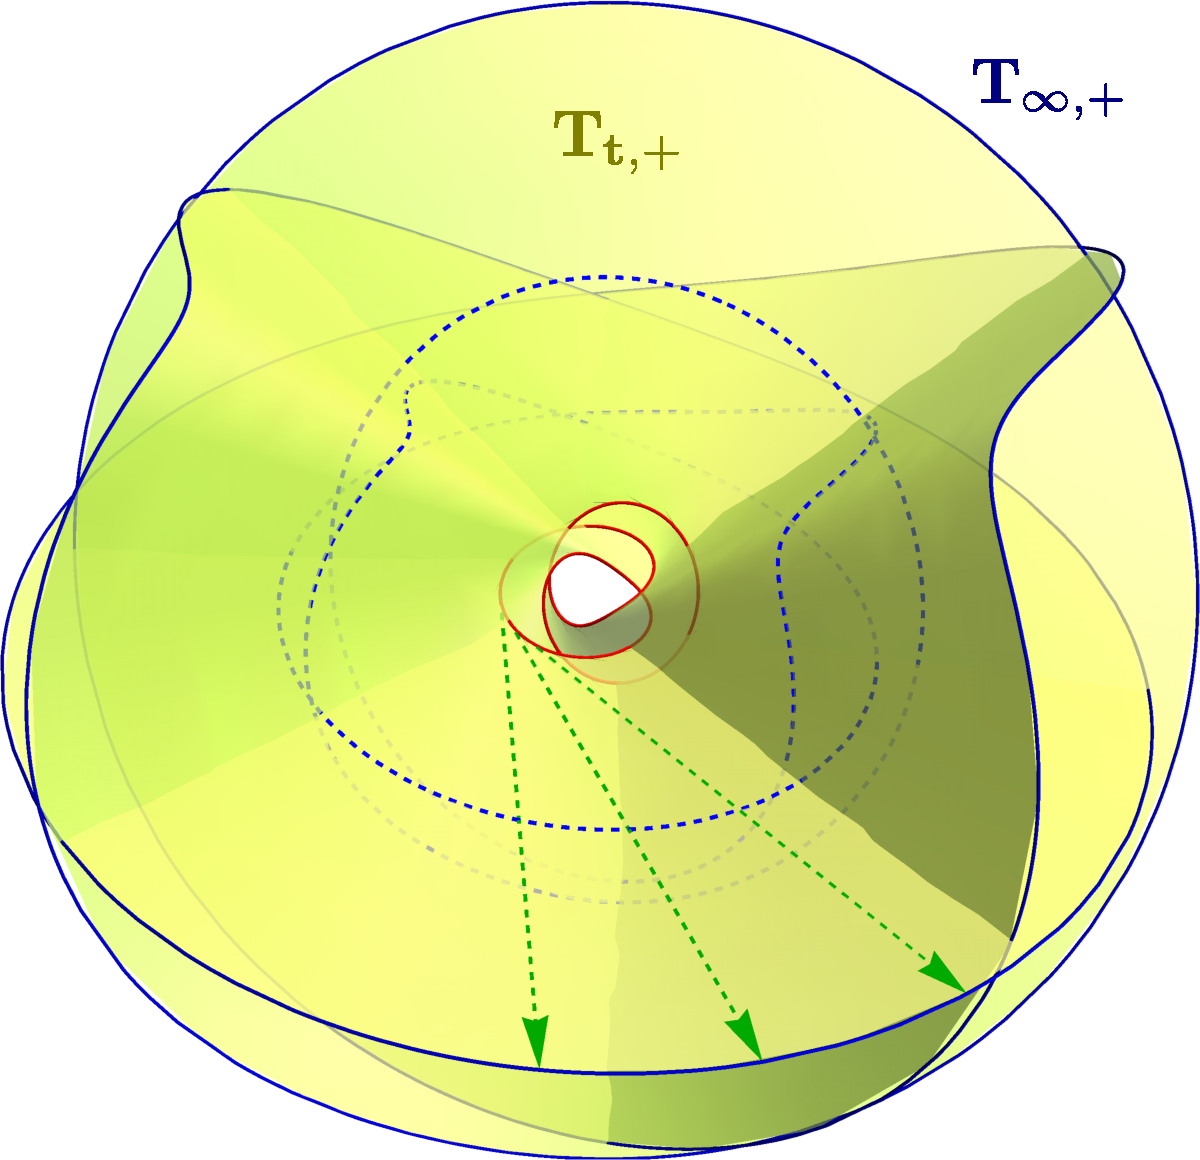
\includegraphics[ width = 0.4\textwidth ]{\MaxwellFigures/Figure5.pdf}
            \caption[Homotopy along the tangent developable surface.]{The forward tangent developable surface ${\bf{T}}_{t,+}$ (yellow surface) for the knot $K$ in figure~\ref{fig:Knot} (red curve), constructed by extending half-lines along tangents from $K$ (green, dashed). The intersection of the surface with a sphere of asymptotically large radius gives a scaled copy of the tangent indicatrix to $K$, ${\bf T}_{\infty,+}$ (blue). The half-lines comprising ${\bf T}_{t,+}$ define a straight line homotopy between $K$ and ${\bf T}_{\infty,+}$, from which the blue, dashed curve is taken.}
            \label{fig:TangentDevelopable}
        \end{centering}
    \end{figure}
    This formula for the solid angle depends only on $K$ and data canonically associated to it, with the only ambiguity being a choice of sign. The appearance of the writhe in~\eqref{eq:OurSolidAngle2} reveals this geometric property of curves to be closely connected to the solid angle. We shall return to the sign ambiguity in a moment --- for now, let us select the plus sign. 

    Instead of taking~\eqref{eq:DualCurve} as our starting point, we now demonstrate how~\eqref{eq:OurSolidAngle2} may be derived directly from the curve homotopy formula~\eqref{eq:Isotopy}. To construct the appropriate homotopy, extend half-lines from $K$ along its tangents ${\bf T}$, sweeping out a surface in space known as the forward tangent developable surface of $K$, which we denote ${\bf{T}}_{t,+}:={\bf y} + t {\bf T}$, $t\in [0,\infty)$~\citep{Eisenhart} --- an example of this surface is shown in figure~\ref{fig:TangentDevelopable}. Consider the intersection of this surface with a sphere of asymptotically large radius. The curve ${\bf T}_{\infty, +}$ given by this intersection is simply the spherical image of $\bf T$, known as the forward tangent indicatrix of $K$ ~\citep{Eisenhart}, scaled to the sphere radius. Our desired homotopy is between $\bf T_{\infty,+}$ and $K$, and is defined by the half-lines comprising ${\bf{T}}_{t,+}$. As $\bf T_{\infty,+}$ is asymptotically far from ${\bf x}$, its projection on to the observation sphere simply reproduces the tangent indicatrix. Using the fact that ${\bf n} \times {\bf T} \cdot \mathrm{d}{\bf n} = 0$, we see that the integral in~\eqref{eq:OurSolidAngle2} is a second special case of~\eqref{eq:Isotopy}, with $K_0 = {\bf T}_{\infty,+}$, $K_1 =K$, and the area swept out on the observation sphere lying between the forward tangent indicatrix and $\bf n$. 

    This argument also identifies $2\pi(1+\mathrm{Wr}(K))$ as the solid angle of $\bf T_{\infty,+}$. We may obtain an integral formula for this area by considering the asymptotics of~\eqref{eq:OurSolidAngle2}, allowing ${\bf x}$ to recede far from $K$ along $-{\bf n}_{\infty}$ so that $\omega({\bf x}) \rightarrow 0$. Doing so yields
    \begin{equation}
        \int_K  \frac{ {\bf n}_\infty \cdot {\bf T} \times \mathrm{d}{\bf T} }{1 + {\bf n}_\infty \cdot {\bf T}} = 2 \pi(1 + \mathrm{Wr}(K))  \quad \textrm{mod}\; 4\pi , 
        \label{eq:AsymptoticSolidAngle2}
    \end{equation}
    however, as this integral is the area bound by the tangent indicatrix on the unit sphere, the identification is simply a recovery of Fuller's writhe mod $2$ formula~\citep{Fuller1978}. In the context of curve homotopies, we may interpret~\eqref{eq:AsymptoticSolidAngle2} as giving the change in solid angle for a homotopy in which $\bf T_{\infty,+}$ shrinks to a point (that projects to ${\bf n}_\infty$ on the observation sphere). Eq.~\eqref{eq:OurSolidAngle2} may then be thought of as a combination of two homotopies: the first from an arbitrary point to $\bf T_{\infty,+}$, and the second from $\bf T_{\infty,+}$ to $K$. By contrast,~\eqref{eq:OurSolidAngle1} combines these two homotopies into one. Returning to the sign choice made above, we now see that choosing a minus sign would give a version of~\eqref{eq:OurSolidAngle2} corresponding to a homotopy along the backward tangent developable surface ${\bf{T}}_{t,-}:={\bf y} - t {\bf T}$, $t\in [0,\infty)$, between $K$ and the backward tangent indicatrix $\bf T_{\infty,-}$. That aside, the geometric interpretation remains the same. We note briefly that the tangent indicatrix is not the only spherical curve canonically associated with $K$ which might be used to define a homotopy; we might also consider the normal and binormal indicatrices. In these cases, however, neither triple product in~\eqref{eq:Isotopy} vanishes, as occurred in~\eqref{eq:OurSolidAngle2}, and so the resulting formulae are less simple. 

    With the choice of plus (minus) sign in~\eqref{eq:OurSolidAngle2}, the surface of discontinuity discussed in \S\ref{sec:CurveIsotopies} is given by ${\bf T}_{t,+}$ (${\bf T}_{t,-}$). Jumps are also present in~\eqref{eq:GaussBonnetImmersed} and~\eqref{eq:DualCurveImmersed}, however they occur on both halves of the tangent developable surface ${\bf T}_{t,+}\cup {\bf T}_{t,-}$ and the overall $4 \pi$ jumps are composed of each individual term in the equations jumping by $2 \pi$. To convince ourselves of this fact, consider the behaviour of~\eqref{eq:DualCurveImmersed} as ${\bf x}$ passes across ${\bf T}_{t,+}\cup {\bf T}_{t,-}$. ${\bf n}$ undergoes a Reidemeister 1 move, during which $D$ jumps by 1. The segment of ${\bf n}^*$ corresponding to the Reidemeister move in ${\bf n}$ begins and ends at antipodal points on the sphere. By removing the loop in ${\bf n}$, we create two inflection points. Recalling that the sign of $ds^*$ alternates between these inflections, we pick up a change in signed length of $2 \pi$.


    \section{The structure of $\omega$}
    \label{sec:LocalStructure}

    The level sets of $\omega$, for regular values, form a family of Seifert surfaces with common boundary $K$. Figure~\ref{fig:SolidAngle} shows this global structure for a twisted unknot and a Whitehead link. 
    The topology of the level sets changes at critical points of $\omega$, where generically the local structure is a cone point $\pm(x^2+y^2-2z^2)$ with Morse index $1$ or $2$. As the solid angle is a harmonic function, critical points of Morse index $0$ or $3$ are forbidden by the maximum principle. For knots and links that are fibred~\citep{Stallings1978} it is possible for the solid angle to have no critical points at all; indeed this is the case for both the unknot and Whitehead link shown in figure~\ref{fig:SolidAngle}. The general relationship between the shape and geometry of a knot or link and critical points of the solid angle is a fascinating open problem. 

    It is of particular interest to characterise $\omega$ in a tubular neighbourhood of $K$, so that we may modify it when initialising simulations using $\omega$. This control is useful when the local structure of the field around a vortex affects its dynamics, as for example in helicity in fluids~\citep{Moffat1992} or the twist of scroll waves in the FitzHugh-Nagumo model~\citep{Winfree1984,Maucher2018}. This local structure has longitudinal and transverse parts: the level sets of $\omega$ rotate as one traverses $K$, and in a plane normal to $K$ corrections due to local curvature and torsion arise, analogous to those studied for the magnetic field about a curved wire~\citep{Saffman1992}. Harmonic fields in the tubular neighbourhood of a knot have also recently been studied in Ref.~\citep{Duan2018}. 

    \begin{figure}[htbp]
        \begin{centering}
            \includegraphics[clip = true, trim = 120 380 120 0, width = 0.9\textwidth ]{\MaxwellFigures/Figure3.pdf}
            \caption[The structure of solid angle around a knotted curve.]{The structure of $\omega$ around a knotted curve, generated with the method of \S\ref{sec:NumericalImplementation}. (a)--(c) show level sets of $\omega$ of spacing $\frac{\pi}{2}$, each of which forms a Seifert Surface for the knot with opacities on the near sides of the images reduced to reveal the inner structure of $\omega$. (a) A twisted unknot. (b,)~(c) The Whitehead link (components in blue, green) from two viewing directions. (d) A slice through the Whitehead link from the same direction as (c). The local structure of $\omega$ about the knot is especially clear in (d) --- $\omega$ winds by $4 \pi$, and as we move away from the knot, curvature induced corrections cause the level sets of $\omega$ to bunch along the curve normal, as discussed in \S\ref{sec:LocalStructure}.}
            \label{fig:SolidAngle}
        \end{centering}
    \end{figure}

    \subsection{Longitudinal structure --- the solid angle framing}
    \begin{figure}[t]
        \makebox[0.9\textwidth][c]{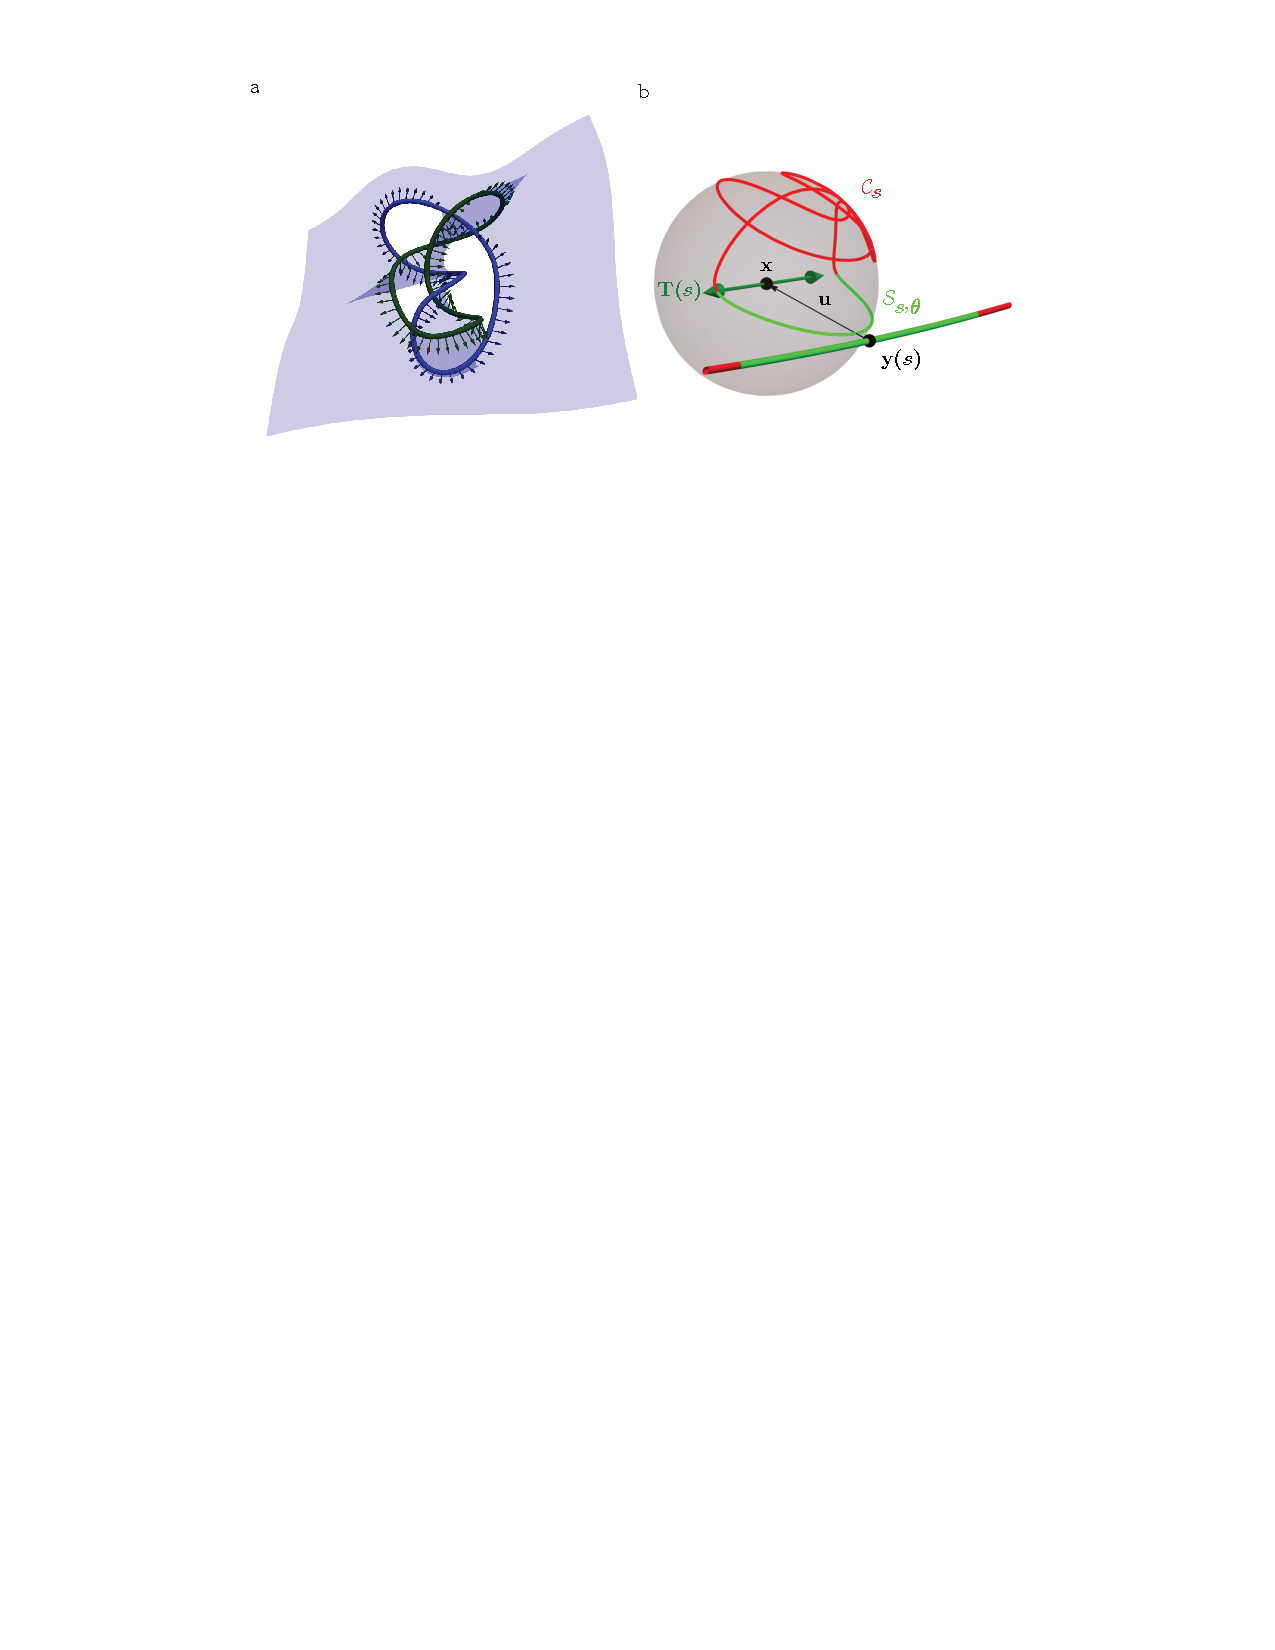
\includegraphics[clip = true, trim = 0 580 0 0, width= \paperwidth ]{\MaxwellFigures/Figure4.pdf}}
        \caption[The solid angle framing.]{(a) The solid angle framing for the Whitehead link of figure~\ref{fig:SolidAngle}. Shown is the level set $\omega =0$ (blue surface), and its induced framing (components in blue, green). (b) The limiting behaviour of $\bf n$ as $\bf x$ approaches $K$ (shown is the behaviour of $\bf n$ about the marked point on the $4_1$ of figure~\ref{fig:Knot}). $\bf x$ approaches a fixed point ${\bf y}(s)$ on $K$ such that ${\bf u} := {\bf x} - {\bf y}(s) = (\epsilon \cos\theta, \epsilon \sin\theta,0)$ lies in the normal plane to ${\bf y} (s)$. As $\epsilon/\rho \rightarrow 0$, a region on $K$ of size $\sqrt{ 2 \rho \epsilon}$ (green) projects to a semicircle $\mathcal{S}_{s,\theta}$ between $\pm{\bf T}(s)$. This semicircle sweeps the observation sphere as $\theta$ is varied. The remainder of $K$ projects to $\mathcal{C}_s$ (red), and is independent of $\theta$.} 
        \label{fig:LocalStructure}
    \end{figure}

    The intersection of the level set $\omega=0$ with $K$ defines a `solid angle' framing, canonical in the sense that it depends only on the knot and is purely geometric. As this framing is described by a pushoff of $K$ onto an orientable surface, it has zero self-linking number~\citep{Lickorish1997}; the extension to links is straightforward and discussed in \S~\ref{sec:NumericalImplementation}. Figure~\ref{fig:LocalStructure}(a) shows this surface and its induced framing for the Whitehead link of figure~\ref{fig:SolidAngle}. A natural question is to identify this solid angle framing in terms of the curve geometry. Let ${\bf x}$ approach a particular point ${\bf y}(s) \in K$, for a fixed $s$, in such a way that the displacement vector ${\bf u} := {\bf x} - {\bf y}(s)$ defines a direction in the normal plane to the curve at $s$ (figure~\ref{fig:LocalStructure}(b)). Aligning the $x,y,z$ axes with the local Frenet-Serret frame ${\bf N}(s),{\bf B}(s),{\bf T}(s)$, we have ${\bf u} = (\epsilon \cos\theta, \epsilon \sin\theta,0)$. As $\epsilon/\rho \rightarrow 0$, where $\rho$ is the radius of curvature, we may think of the image of $K$ on the observation sphere as comprised of two parts; for points ${\bf y}(s')$ with $s'$ outside a small interval $I$ around $s$ (of size $\sim\sqrt{2\rho \epsilon}$), the projection to ${\bf x}$ is no different from the projection to ${\bf y}(s)$, and the image of $K$ is given by the unit chords $\frac{{\bf y}(s') - {\bf y}(s)}{|{\bf y}(s') - {\bf y}(s)|}$. This is a curve $\mathcal{C}_s$ on the observation sphere with endpoints $\pm {\bf T}(s)$ and is independent of $\theta$. In the same limit, the points ${\bf y}(s^{\prime})$ with $s^{\prime}\in I$ contribute to the image of $K$ on the observation sphere a semicircle $\mathcal{S}_{s,\theta}$ between $\pm{\bf T}(s)$ with midpoint $- \frac{{\bf u}}{|{\bf u}|}$ that depends on $\theta$. ${\bf n}$ is thus decomposed as ${\bf n} = \mathcal{C}_s \cup \mathcal{S}_{s,\theta}$. Varying $\theta$, $\mathcal{C}_s$ remains unchanged, and $\mathcal{S}_{s,\theta}$ wraps the sphere once, giving the asymptotic winding structure $\omega = 2(\theta - \alpha(s))$, where $\alpha(s)$ is the rotation angle of the Frenet-Serret normal ${\bf N}(s)$ into the solid angle framing. $\alpha(s)$ gives the longitudinal structure of $\omega$. It represents the contribution of $\mathcal{C}_s$ to $\omega$, and as such is a global quantity, not computable by a local analysis. 

    Our decomposition of ${\bf n}$ is identical to that of the set of cross chords considered in the context of C\u{a}lug\u{a}reanu's theorem~\citep{Dennis2005,Calugareanu1959}, a consequence of the projection map outside of $I$ degenerating to the chord map as $\epsilon/\rho \rightarrow 0$ to give $\mathcal{C}_s$. The completion of $\mathcal{C}_s$ by $\mathcal{S}_{s,\theta}$ is given, in C\u{a}lug\u{a}reanu's theorem, by a choice of framing vector ${\bf u}$ for $K$~\citep{Dennis2005}. Here it is given, via projection, by the displacement vector ${\bf u}$.

    As discussed by Dennis \& Hannay in Ref.~\citep{Dennis2005}, given some framing ${\bf u}$, $\mathrm{Wr}(K)$ and $\mathrm{Tw}(K, {\bf u})$ are given by the areas swept out on an abstract sphere by $\mathcal{C}_s$ and $\mathcal{S}_{s,\theta}$ respectively, as $s$ varies along $K$. They point out that one may choose a special framing, which they call the `writhe framing', such that the area swept out by $\mathcal{S}_{s,\theta}$ precisely cancels that swept out by $\mathcal{C}_s$, giving zero self-linking number. The discussion above makes clear this framing is exactly the solid angle framing, and the cancellation condition may be naturally read as a variation of $\theta$ such that $\frac{{\bf u}}{|{\bf u}|}$ lies tangent to the level set $\omega = 0$; in terms of the Frenet-Serret frame, $\theta= \alpha(s)$.

    \subsection{Transverse structure --- curvature induced corrections to $\omega$}

    In the previous section, we saw that the asymptotic structure of $\omega$ normal to $K$, corresponding to the decomposition ${\bf n} = \mathcal{C}_s \cup \mathcal{S}_{s,\theta}$, is simply $\omega = 2( \theta - \alpha(s))$. At finite $\epsilon/\rho$ we find corrections due to the local curvature of $K$, with the leading contribution being logarithmic in $\epsilon$. For the derivative of $\omega$, the magnetic field, this problem is well studied \citep{Saffman1992,Ricca1994}. However, we wish to demonstrate that existing results may be mapped directly on to corrections in the geometry of $\bf n$ as the decomposition ${\bf n} = \mathcal{C}_s \cup \mathcal{S}_{s,\theta}$ is smoothed at finite $\epsilon/\rho$, insight one does not gain from the magnetostatic picture.

    The asymptotic description ${\bf n} = \mathcal{C}_s \cup \mathcal{S}_{s,\theta}$ contains cusps at the boundary between $\mathcal{C}_s$ and $\mathcal{S}_{s,\theta}$, located at $\pm {\bf T}(s)$. The primary effect of small but finite $\epsilon/\rho$ is a rounding of these cusps, and the displacement of ${\bf n}$ slightly off $\pm {\bf T}(s)$, as shown in figure~\ref{fig:CurvatureCorrections}(a). It is thus natural to focus our attention, and chose coordinates, appropriate to describing $\bf n$ in the vicinity of $\pm {\bf T}(s)$. Expanding ${\bf y}(s')$ to lowest order in $s'$, ${\bf y}(s') = (\frac{1}{2\rho}(s'-s)^2,0,s'-s)$ and $\bf n$ is given by
    \begin{equation}
        {\bf n} = \biggl[1 + \frac{\tilde{\epsilon}}{2} \biggr(\tilde{s}^2 +\frac{1}{\tilde{s}^2}\biggl)- \tilde{\epsilon}\cos \theta \biggr]^{-\frac{1}{2}} 
        \biggr(
        \sqrt{\frac{\tilde{\epsilon}}{2}}\frac{1}{\tilde{s}} (\tilde{s}^2 - \cos \theta),
        -\sqrt{\frac{\tilde{\epsilon}}{2}}\frac{1}{\tilde{s}} \sin \theta,
        1
        \biggl),
        \label{eq:FirstCurvatureCorrectedn}
    \end{equation}
    where we have defined reduced lengthscales $\tilde{\epsilon}:=\frac{\epsilon}{\rho}$, $\tilde{s} :=\frac{s'-s}{\sqrt{2\epsilon \rho}}$. The form of~\eqref{eq:FirstCurvatureCorrectedn} is chosen to emphasise that we have an expansion of $\bf n$ in the vicinity of $\pm{\bf T}(s)$ on the observation sphere. Focusing now on the smoothed cusp at positive $\tilde{s}$, we introduce a new variable $t :=\ln(\tilde{s})$, and rotate the $x$-$y$ coordinates of ${\bf n}$ by $\frac{\theta}{2}$, yielding 
    \begin{equation}
        {\bf n}
        = [1 + \tilde{\epsilon}(\cosh 2t - \cos \theta )]^{-\frac{1}{2}}
        \biggr(
        \sqrt{2\tilde{\epsilon}} \cos \frac{\theta}{2} \sinh t, 
        -\sqrt{2\tilde{\epsilon}}\sin \frac{\theta}{2} \cosh t,
        1
        \biggl),
        \label{eq:CurvatureCorrectedn}
    \end{equation}
    a hyperbola projected onto the observation sphere (figure~\ref{fig:CurvatureCorrections}(a)). In the original, unrotated coordinates, the asymptotic behaviour of this hyperbola is of two longitudinal great circles passing through ${\bf T}(s)$ at angles $\theta$ and $0$. As $\tilde{\epsilon}\rightarrow 0$, the first of these circles gives $\mathcal{S}_{s,\theta}$. The second gives the local structure of $\mathcal{C}_s $, and in particular tells us that the direction of departure of $\mathcal{C}_s$ from ${\bf T}(s)$ is set by ${\bf N}(s)$. The vertex of the hyperbola, found at $t = 0$, is the point of closest approach to ${\bf T}(s)$ and gives the natural choice $\tilde{s} =1$ ($s' = s + \sqrt{2\rho \epsilon}$) to define the upper boundary between $\mathcal{S}_{s,\theta}$ and $\mathcal{C}_s $. It approaches the pole as $\sqrt{{\tilde{\epsilon}}}$, and so in the limit $\tilde{\epsilon} \rightarrow 0$ we recover the sharp decomposition ${\bf n} = \mathcal{C}_s \cup \mathcal{S}_{s,\theta}$.

    The local structure of the solid angle can be computed using any of our formulae for $\omega$, however, in view of the foregoing description, an appealing method is to use~\eqref{eq:GaussBonnetImmersed} and the geodesic curvature of the hyperbola. As this approach is symmetric in $\tilde{s}$, it is enough to compute the geodesic curvature for the hyperbola near $\tilde{s}=1$ and simply double the result to account for $\tilde{s}=-1$. Further, the geodesic curvature of $\bf n$ is strongly peaked in a localised region of size $\sim\sqrt{\tilde{\epsilon}}$ about the vertex of the hyperbola, decaying to $0$ as the hyperbola approaches its asymptotic great circles. 
    Using~\eqref{eq:CurvatureCorrectedn} we find an integrated geodesic curvature of 
    \begin{equation}
        -2 \int_{-\infty}^{\infty}\frac{\sin \theta\sqrt{1+\tilde{\epsilon}( \cosh 2t - \cos \theta)} }{\cos \theta + \cosh 2t + \tilde{\epsilon} \sin^2 \theta } \mathrm{d}t,
        \label{eq:CurvatureCorrectionIntegration}
    \end{equation} 
    where we have extended the upper limit of integration to $+\infty$, corresponding to an integration of the hyperbola between $- \frac{{\bf u}}{|{\bf u}|}$ and ${\bf N}(s)$ on the observation sphere. The integrand decays exponentially for large $t$ so that the error involved is small. 

    The integral~\eqref{eq:CurvatureCorrectionIntegration} may be evaluated exactly in terms of elliptic integrals of the first and third kind. The main feature is that the result is not analytic in $\tilde{\epsilon}$ but has leading behaviour $\tilde{\epsilon} \ln \tilde{\epsilon}$. This can be seen most easily by noting that the integrand decays exponentially for $|t| \gtrsim \frac{1}{2} \ln (2/\tilde{\epsilon})$ and that the integral is dominated by values of $|t|$ smaller than this. 
    Retaining only the leading behaviour, one finds the local structure of the solid angle has the form 
    \begin{equation}
        \omega(\tilde{\epsilon}, \theta)= 2 \bigl( \theta-\alpha(s) \bigr) + \tilde{\epsilon} \ln \frac{8}{\tilde{\epsilon}}\, \sin \theta + O(\tilde{\epsilon}) ,
        \label{eq:CurvatureCorrection}
    \end{equation} 
    in which a zeroth order term from the integrated geodesic curvature gives the winding of $\omega$ and the logarithmic term causes the level sets of $\omega$ to bunch along the local normal. Figure~\ref{fig:SolidAngle}(d) shows a cross-section through a Whitehead link in which both of these structures are clearly visible. In figure~\ref{fig:CurvatureCorrections}(b) we compare the various orders of approximation in~\eqref{eq:CurvatureCorrection} to the exact solution for a round unknot. In contrast to the divergence of the magnetic field, $\omega$ is perfectly well behaved as $\tilde{\epsilon} \rightarrow 0$. The logarithmic correction $\tilde{\epsilon} \log \tilde{\epsilon}$ tends to $0$, but in a cusped manner, with unbounded radial derivative at the origin. We may interpret this fact as a direct consequence of the limiting cusped structure ${\bf n} = \mathcal{C}_s \cup \mathcal{S}_{s,\theta}$ --- the magnetic field gives the rate of change in the area of a spherical curve as we smooth a cusp in it, and is thus naturally unbounded. 

    We note briefly that~\eqref{eq:CurvatureCorrection} is not harmonic --- indeed, the corresponding expression for the magnetic field found in, for example, \citep{Saffman1992} is not divergence free. This is a consequence of neglecting variation in $\omega$ along ${\bf T} (s)$ and one may verify that, allowing $\bf {x}$ to lie off the plane normal to ${\bf y}(s)$, one picks up a term linear in $z$ which restores harmonicity. 

    \begin{figure}[htbp]
        \begin{centering}
            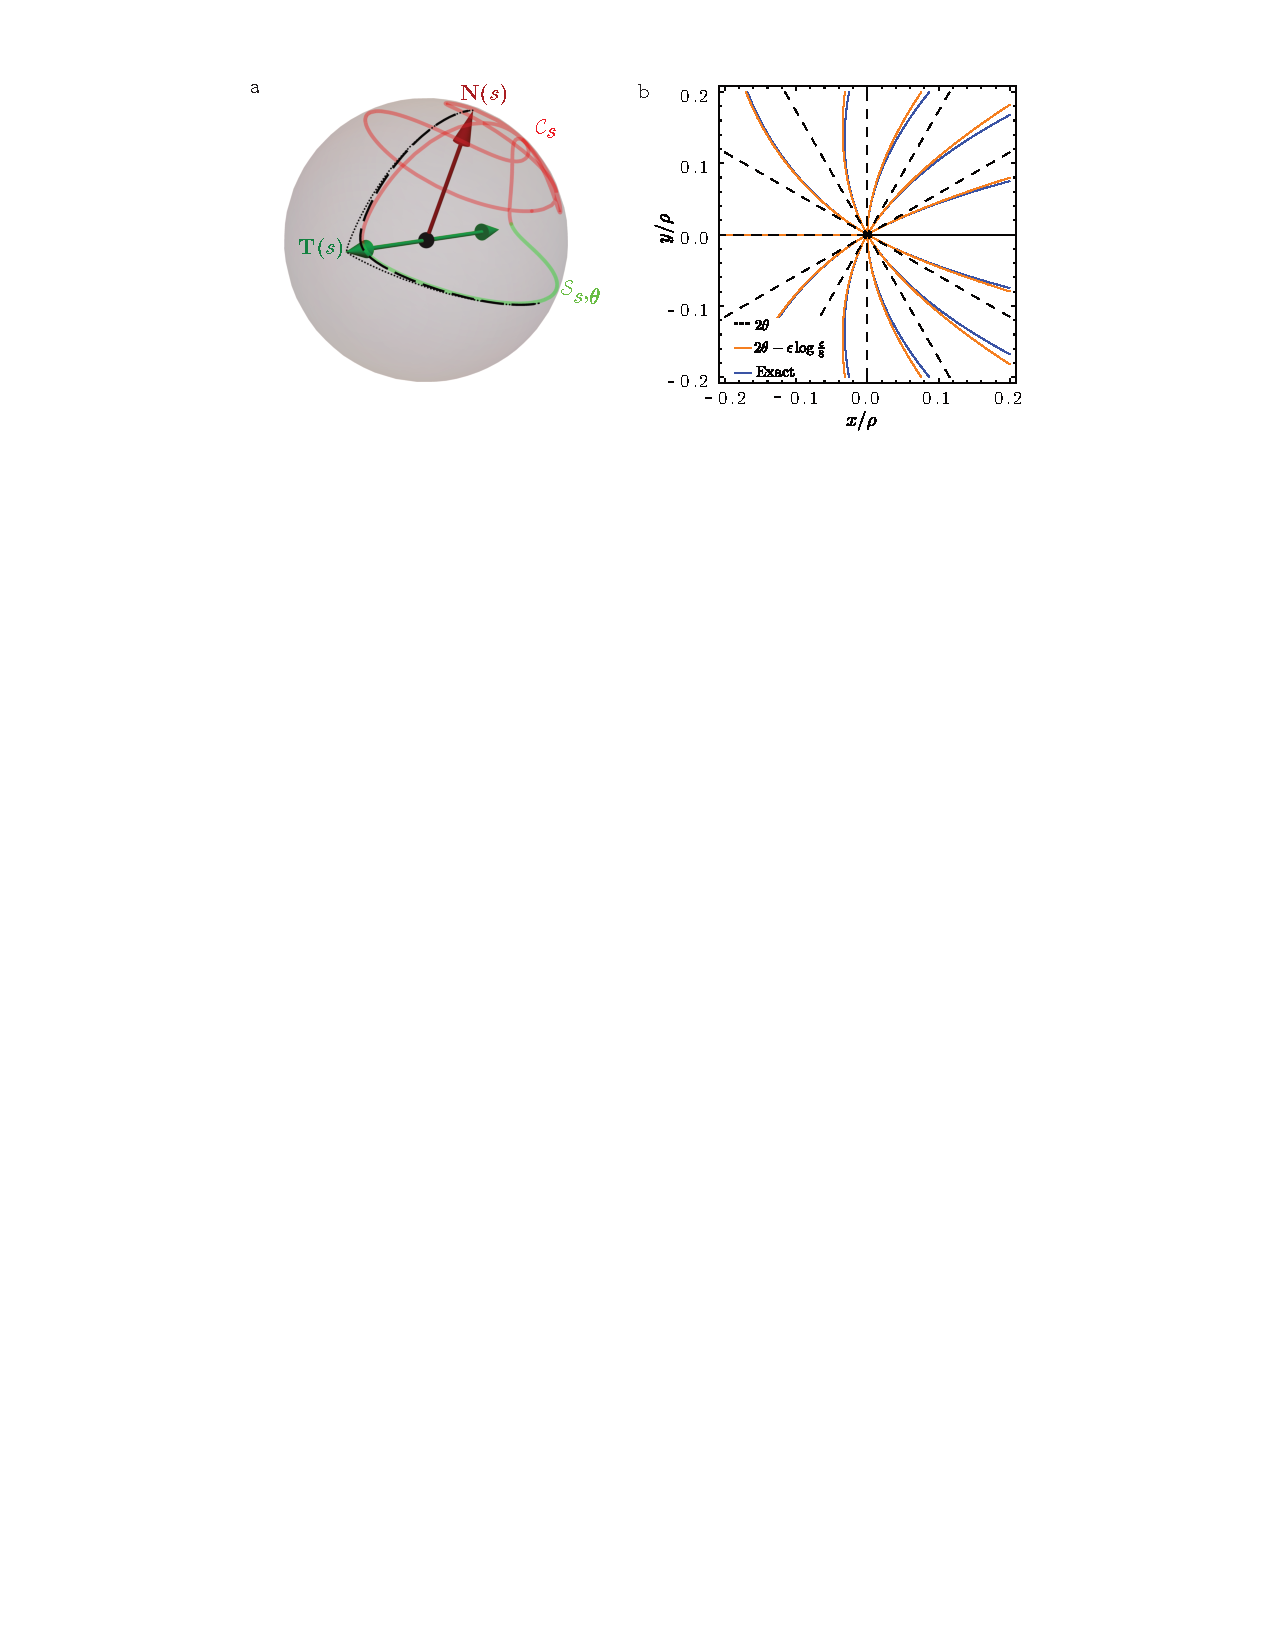
\includegraphics[clip = true, trim = 120 580 120 0, width = 0.9\textwidth ]{\MaxwellFigures/Figure6.pdf}
            \caption[Transverse solid angle structure.]{(a) For finite $\epsilon/\rho$, the local structure of $\bf n$ is approximated by the hyperbola~\eqref{eq:CurvatureCorrectedn} --- the dashed black line gives the approximation to $\bf n$ shown in figure~\ref{fig:LocalStructure}. As $\epsilon /\rho \rightarrow 0$, the vertex of this hyperbola approaches ${\bf T}(s)$, and the asymptotes remain unchanged (black dotted line). In this way, we obtain the limiting decomposition ${\bf n} = \mathcal{C}_s \cup \mathcal{S}_{s,\theta}$. The two asymptotes are great circles through ${\bf T}(s)$ at angles $\theta$ and $0$, and give the local behaviour of $\mathcal{S}_{s,\theta}$ and $\mathcal{C}_s$ --- note that that an angle of $0$ corresponds to the direction ${\bf N}(s)$. (b) The local structure of $\omega$ in a plane normal to $K$. Contours of spacing $\frac{\pi}{3}$ are shown for the the zeroth order rotational structure (black dashed line), the curvature induced correction~\eqref{eq:CurvatureCorrection} (green) and the exact solution for a circle of radius $\rho$ (blue). The absolute values of the level sets are arbitrary, as we have discarded global information about $\mathcal{C}_s$ in our local structure calculations. The primary effect of curvature is to bunch the level sets of $\omega$ along the local normal. Note that for the curvature induced correction we have fixed the regular values in~\eqref{eq:CurvatureCorrection} to zero by comparison with the exact solution for a circle \citep{Saffman1992}.}
            \label{fig:CurvatureCorrections}
        \end{centering}
    \end{figure}

    \section{Remarks on numerical implementation, extension to links}
    \label{sec:NumericalImplementation}

    In~\eqref{eq:OurSolidAngle1},~\eqref{eq:GaussBonnetImmersed},~\eqref{eq:DualCurveImmersed} and~\eqref{eq:OurSolidAngle2}, we have several possible methods for computing $\omega$ for any curve $K$, directly from the specification of its embedding in $\mathbb{R}^3$. The main difficulties in their numerical implementation are encountered when evaluating $\omega(\bf x)$ at points close to the surface of discontinuity discussed in \S\ref{sec:CurveIsotopies}, \ref{subsec:Pullback}. We shall focus discussion on~\eqref{eq:OurSolidAngle1} and~\eqref{eq:OurSolidAngle2}, the remaining equations being of similar numerical character.

    Focusing first upon~\eqref{eq:OurSolidAngle1}, when $\bf x$ lies on the surface of discontinuity it is pierced by a (generically) unique half-line extended from some point ${\bf y}(s) \in K$ such that ${\bf n}(s) \cdot {\bf n}_\infty = -1$. Considering the integral in~\eqref{eq:OurSolidAngle1} to be defined upon $K$, at the arc length $s$ there is an isolated point of divergence in the integrand. In the degenerate case where ${\bf x}$ lies upon a line of self-intersection in the surface, there will be multiple such points. Letting ${\bf x}$ now lie slightly off the surface and approach it perpendicularly, we may expand the integrand of~\eqref{eq:OurSolidAngle1} using ${\bf x}-{\bf y}(s) := \epsilon \cos \theta\, {\bf n}_\infty + \epsilon \sin \theta\, {\bf n}_\infty \times {\bf T}(s) / |{\bf n}_\infty \times {\bf T}(s)| $, where $\theta$ is now the angle between $ {\bf x}-{\bf y}(s)$ and the surface. We find that its limiting behaviour is that of a Lorentzian peak of width $\epsilon \theta$, which abruptly switches sign as ${\bf x}$ crosses the surface. If one employs a simple numerical integration scheme with regularly spaced points along $K$ of spacing $\Delta s$, the Lorentzian peak is not captured when $\epsilon \theta \approx \Delta s$. This leads to poor approximation of $\omega({\bf x})$ in a region of constant thickness $\Delta s$ about the surface of discontinuity. By refining $K$, we may reduce the thickness of this region --- unsurprisingly, this result suggests that $\Delta s$ should be on the order of the resolution one desires for $\omega$.

    A similar discussion holds for~\eqref{eq:OurSolidAngle2}, for which the divergences of the integrand occur at $s$ such that ${\bf n}(s)\cdot{\bf T}(s) = \pm 1$, depending on which homotopy is used. The width of the Lorentzian peak instead scales as $\rho(s) \theta$, and so the thickness of the region of poor approximation is $\Delta s \epsilon/ \rho (s)$; in particular, we note that this thickness scales with viewing distance in~\eqref{eq:OurSolidAngle2}, but not in~\eqref{eq:OurSolidAngle1}.

    One method of avoiding these peaks is to use the freedom in~\eqref{eq:OurSolidAngle1},~\eqref{eq:OurSolidAngle2} to move the surface of discontinuity about in space, ensuring ${\bf x}$ is never too close to it when computing $\omega({\bf x})$. In~\eqref{eq:OurSolidAngle1}, we have freedom in our choice of ${\bf n}_\infty$. The surface of discontinuity is given by dragging $K$ to infinity along ${\bf n}_\infty$, and two different choices of ${\bf n}_\infty$ will give two such surfaces. If $K$ is knotted, these surfaces must intersect, giving a set of curves on which a third choice of ${\bf n}_\infty$ is needed. In practice, an initial choice of ${\bf n}_\infty$ is often suggested by the geometry of the input knot, or is simply chosen to be a coordinate axis. When computing $\omega({\bf x})$, one may record the minimum value of ${\bf n}\cdot {\bf n}_\infty$ and, if it crosses some user defined threshold, switch to using $-{\bf n}_\infty$ for the calculation at that point. On the set of lines where this second choice again crosses the threshold, a random choice of ${\bf n}_\infty$ may be used.~\eqref{eq:OurSolidAngle2} faces analogous problems on the tangent developable surface. Here, we have freedom in whether to place the discontinuity on ${\bf T}_{t,+}$ or ${\bf T}_{t,-}$. However, these two surfaces again generically intersect \citep{Cleave1980,Mond1989}, and there is now no more freedom in $\eqref{eq:OurSolidAngle2}$, forcing one to either switch method or analytically correct for the Lorentzian peaks along such intersections. For this reason, and for the scaling properties discussed above, from a numerical standpoint we have found the use of~\eqref{eq:OurSolidAngle1} to be more convenient than~\eqref{eq:OurSolidAngle2}. 

    Two brief computational remarks: As discussed in \S\ref{sec:LocalStructure}, the limiting local structure of $\omega$ about $K$ has cylindrical symmetry. If one desires high accuracy to sample the tubular neighbourhood of $K$, one may use a cylindrical mesh out to a distance ${\sim}\rho(s)$. Finally, we note that as values of $\omega$ for different values of $\bf x$ are computed independently of one another, our formulae are easily parallelised. 

    \subsection{Extension to links}
    Extending our results to links is straightforward: by the linearity of electromagnetism, one simply sums $\omega$ mod $4 \pi$ for each component of $K$. We reiterate that $\omega$ is only defined for oriented curves, and that different choices of orientation for each component of $K$ will give distinct solid angle functions. In the case of the solid angle framing discussed in \S\ref{sec:LocalStructure}, each component $K_i$ acquires a framing, whose self-linking number equals the negative of the sum of the linking numbers between $K_i$ and $K_j$, $j \neq i$ (figure~\ref{fig:LocalStructure}).

    \section{Construction of knotted fields: two illustrations}

    We describe briefly two different examples of knotted fields that can be constructed using the solid angle as illustrations of how it influences the structure in different settings. 

    \subsection{Scroll waves in excitable media}
    \label{subsec:scroll}

    The possibility of knotting in the waves of excitable media has been considered for some time~\citep{Winfree1983,Winfree1984}. In a three-dimensional excitable medium, scroll waves of excitation emanate from a vortex filament, which it is possible to close into a loop or knot. Recent results have highlighted a remarkable topology-preserving dynamics in these materials~\citep{Maucher2016,Maucher2017,Maucher2018} in which the geometric shape of the vortex filament relaxes and simplifies but without strand crossings, thus preserving the topology. Simple effective curve dynamics seem insufficient to capture the full behaviour, which depends also on interactions mediated by the global structure of the scroll waves. This structure can be captured, in part at least, using the solid angle. 

    \begin{figure}[htbp]
        \centering
        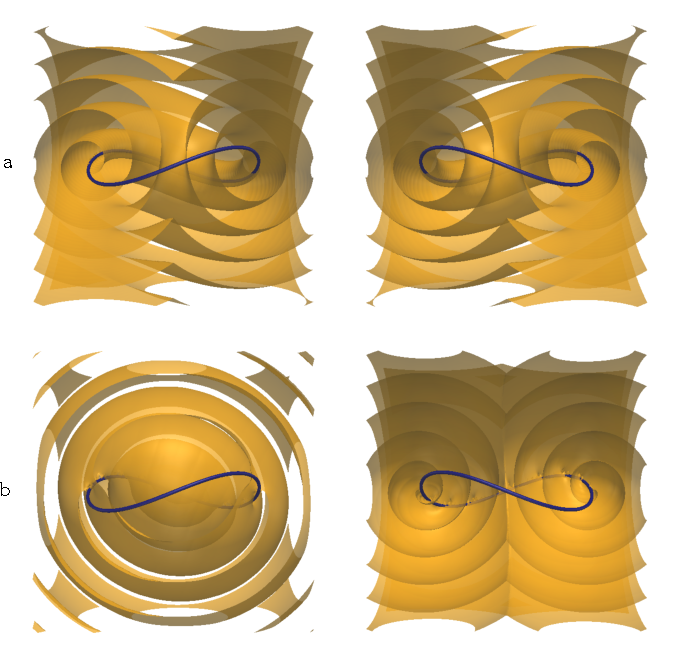
\includegraphics[width=.5\textwidth]{\MaxwellFigures/Figure7}
        \caption[Constructing scroll waves from solid angle.]{Scroll waves from a unknotted vortex filament. In (a) we show the zero level set of the phase field~\eqref{eq:scroll} and in (b) a modification of it where a sinusoidal modulation has been added to the solid angle framing, thereby adjusting the local spin rate of the scroll wave. In both (a) and (b) the two columns simply show different cuts through the emanating scroll waves.}
        \label{fig:scroll}
    \end{figure}

    Scroll waves emanate from a knotted vortex filament creating an outward propagating family of approximately equi-spaced wavefronts. A simplified description of this wave system is given by a phase field that both winds by $2\pi$ around the filament curve and increases linearly with distance from it. This behaviour is captured by the function 
    \begin{equation}
        \psi({\bf x}) = k d_{K}({\bf x}) + \frac{1}{2} \omega_{K}({\bf x}) \quad \textrm{mod}\; 2\pi ,
        \label{eq:scroll}
    \end{equation} 
    where $\omega_K({\bf x})$ is the solid angle of $K$, $d_{K}({\bf x}) = \min_{{\bf y} \in K} |{\bf y}-{\bf x}|$ is the distance from ${\bf x}$ to the curve $K$ and $k$ is a wavenumber. In figure~\ref{fig:scroll}(a) we show an example of the scroll waves generated by a simple unknotted vortex ring. 
    Note that the way the wave surface attaches to the filament -- {\sl i.e.} the local spin rate of the scroll wave along the length of the filament -- is determined by the solid angle and, in particular, given by the solid angle framing. Of course, the phase function~\eqref{eq:scroll} can be modified to vary this; the modulation can by thought of as a $K$-dependent off-set to the distance function $d_{K}({\bf x})$. An example of such a modulation and how it alters the scroll waves is shown in figure~\ref{fig:scroll}(b). 

    \subsection{Nematic disclinations}
    \label{subsec:nematics}

    In nematic liquid crystals it is possible to manipulate topological defect lines, called disclinations, so as to create closed loops in the form of any knot or link~\citep{Tkalec2011,Copar2015,Machon2013}. The surrounding liquid crystal texture is an example of a knotted field. 
    The molecular orientation in liquid crystals is described by a unit vector ${\bf d}$ with the nematic symmetry ${\bf d} \sim - {\bf d}$; disclinations are line defects in the director field around which the orientation rotates by $\pi$, or reverses. 
    The solid angle facilitates an explicit construction of a knotted field with this property. For example, the director field 
    \begin{equation}
        {\bf d}({\bf x}) = \bigl[ \sin\bigl( \omega_{K}({\bf x}) / 4 \bigr) , 0 , \cos\bigl( \omega_{K}({\bf x}) / 4 \bigr) \bigr], 
        \label{eq:planar_nematic}
    \end{equation}
    encodes $K$ as a disclination line for any choice of knotted curve, or link. This knotted field has two particularly notable properties. First, since the solid angle is harmonic, it corresponds to a critical point of the one elastic constant Frank free energy. Second, the texture is ``planar'', having no $y$-component. 

    \begin{figure}[htbp]
        \centering
        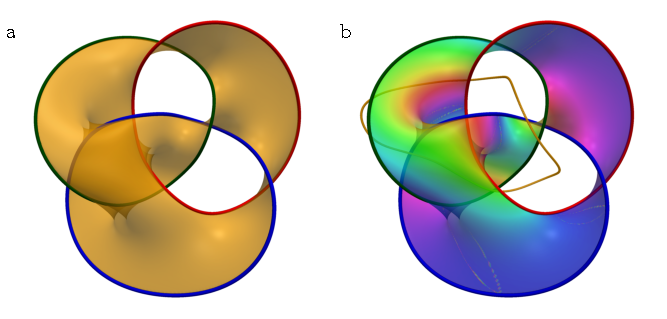
\includegraphics[width=\textwidth]{\MaxwellFigures/Figure8.pdf}
        \caption[Constructing knotted nematic disclinations from solid angle.]{Knotted nematic texture for disclinations forming the Borromean rings. The surface corresponds to the set of points where the director has no $z$-component, $d_z=0$; it is coloured according the $xy$-components. In (a) the texture is planar (Eq.~\eqref{eq:planar_nematic}) and in (b) it is fully three-dimensional (the curve defining the $xy$-winding through the angle $\omega_L$ is also indicated).}
        \label{fig:nematic}
    \end{figure}

    We show in figure~\ref{fig:nematic}(a) a visualisation of the director field~\eqref{eq:planar_nematic} for the case where the disclination lines $K$ correspond to the Borromean rings. The knotted nematic texture is conveniently visualised by showing the surface where the $z$-component of the director vanishes --- the vector field~\eqref{eq:planar_nematic} has boundary conditions such that the director is aligned along $z$ asymptotically far from $K$, motivating this choice. This surface is a level set of the solid angle, namely $\omega_{K}=2\pi$. 

    A generalisation creating fully three-dimensional knotted nematics is the vector 
    \begin{equation}
        \fl    {\bf d}({\bf x}) = \biggl[ \sin\biggl(\frac{\omega_{K}({\bf x})}{4}\biggr) \cos\biggl(\frac{\omega_{L}({\bf x})}{2}\biggr) , \sin\biggl(\frac{\omega_{K}({\bf x})}{4}\biggr) \sin\biggl(\frac{\omega_{L}({\bf x})}{2}\biggr) , \cos\biggl(\frac{\omega_{K}({\bf x})}{4}\biggr)  \biggr] ,
        \label{eq:nonplanar_nematic}
    \end{equation}
    where $\omega_{L}({\bf x})$ is a second solid angle function for a curve $L$ chosen as follows. The surface $d_z=0$ is the same as before (the level set $\omega_{K}=2\pi$) but the director field is no longer constant over it, varying with the solid angle function $\omega_{L}$. In figure~\ref{fig:nematic}(b) we illustrate this through the colour of the surface. Now the gradient of this colour is (proportional to) a magnetic field and $L$ is the curve corresponding to the current carrying wire needed to generate that magnetic field. More formally, $L$ is a curve in the complement of the surface $d_z=0$ corresponding to a homology cycle and generates colour winding around the dual cycle of the surface itself. Knotted nematic fields with any desired topological properties can be constructed in this way but of course the construction is more than purely topological and depends also on the geometric properties of the solid angle and of the curves that generate them. 

    \section{Discussion}
    \label{sec:discussion}

    The solid angle provides a canonical knotted field for any explicitly given curve or link, depending only on that curve and its geometry. As such it facilitates a study of the geometry of knotted fields, shedding light on their structure and establishing connections between the field and the geometry of the curve. 
    We have given a survey of its properties and methods for computing it that parallels and modernises Maxwell's seminal presentation. 
    The fundamental result is the homotopy formula~\eqref{eq:Isotopy}, which unifies the different formulae for calculating the solid angle, and also provides the means for characterising changes in the knotted field induced by deformations of the curve. In the latter context, it would be natural to study the consequences of inflection points and other geometric degeneracies in the curve shape, and also strand crossings or, with suitable extension, reconnections. Likewise, one could seek a characterisation of the geometric shape of a knot or link whose solid angle function realises specific properties, for instance having a minimal number of critical points. Those special geometric shapes where the properties of the solid angle change would then represent an interesting branch of singularity theory. 

    The local structure of the field can be considered particularly important in many systems. Here, the natural framing provided by the solid angle and its relation to the writhe of the curve establish a standard reference, from which the global effects of changes to the local behaviour can be systematically assessed. 


 \chapter{Stable and Unstable Vortex Knots in Excitable Media}
\label{ch:FitzHughNagumo}
\section{\label{sec:Introduction}Introduction}
Models of excitable media support spiral wave vortices in two dimensions\footnote{The introduction to this chapter is self-contained. However, for much more detail on excitable media, and the theory and history of vortex knots inside them, the reader should see \S\ref{sec:FN}, with which this section and \S\ref{sec:Methodology} share a little overlap.}. In a three-dimensional medium the analogous structure is a vortex filament~\citep{Winfree1983}. Such a filament may close on itself to form, in the simplest case, an unknotted loop, and more generally a knotted vortex~\citep{Winfree1983b}. As well as being organising centres for waves of excitable activity, early numerical experiments and theoretical work showed that these knotted filaments have their own dynamics~\citep{Keener1988,Winfree1990, Keener1992,Henze1993, Biktashev1994,WinfreeChapter,Dierckx2010}. Remarkably, in a simple example of an excitable medium, the FitzHugh-Nagumo model, simulations suggested that these dynamics were topology preserving, and further that they were capable of `simplifying' a knot, reducing an initially complicated filament geometry to a simpler stationary state~\citep{Winfree1990,Henze1993,WinfreeChapter}. Such a scenario stands in stark contrast to the knot untying via reconnection events seen in other examples of knotted fields such as fluids and superfluids~\citep{Kleckner2013,Scheeler2014,Kleckner2016}. 

So far, the striking knot simplification has been reported only for the unknot~\citep{Maucher2016} --- reducing three examples of tangled, but unknotted, curves to a geometric circle of fixed average radius --- and, in two examples, the trefoil~\citep{Sutcliffe2003,Maucher2016}. At higher crossing number the behaviour appears to be more complicated. Nevertheless, with the exception of two examples discussed below, reported knot and link evolutions are still consistent with preservation of topology~\citep{Henze1993, Winfree1990, WinfreeChapter, Sutcliffe2003,Maucher2016,Maucher2017, Maucher2019}. Stationary states have been reported for all torus knots and links up to $N=12$~\citep{Maucher2017,Maucher2019}, where $N$ denotes the crossing number of the knot or link, although only in the case where they are stabilised by proximity to a planar surface with Neumann (no-flux) boundary conditions and the vortex filaments are initialised to have the idealised geometry of torus curves. Both of these features are believed to be important for the stability of these examples~\citep{Maucher2017,Maucher2019}. If the vortex is initialised with idealised torus geometry but not sufficiently close to the boundary, it is prone to poorly understood instabilities which cause it to deviate from the initially symmetric form. Similarly, torus knots initialised without the idealised geometry do not evolve to the observed stationary states and instead follow irregular dynamics, typically ending with the filament breaking upon contact with the no-flux surface. It is not known how close to the idealised torus geometry the initial curve needs to be to attain the stationary state. A cautionary example is provided by early bulk (not close to a no-flux boundary) simulations of a variety of knots and links, including torus knots, started from exactly symmetric configurations, which appeared stable over the times initially simulated~\citep{Henze1993}. As we shall demonstrate in the case of torus knots, over longer timescales such geometries in fact destabilise. The recent no-flux simulations are over much longer timescales, however in the absence of theoretical results it is not clear exactly how long simulations testing knot stability should be.

As indicated above, in contrast to topology preserving dynamics seen in the unknot some apparently exceptional examples of topological non-preservation have been reported, the first being the already discussed example of a single filament breaking at a no-flux boundary, effectively interacting with its mirrored neighbour. In the bulk, a small vortex loop (stable in isolation) may be annihilated by a larger coaxial one ~\citep{Courtemanche1990,Maucher2018}. The mechanism behind this annihilation is thought to be `wave slapping' by a train of high frequency wavefronts coming from the larger loop impacting upon the smaller one (which has a vortex rotation frequency below that seen for an isolated filament) causing it to destabilise.

Underlying all of the above observations are general questions as to the driving factors behind knot dynamics, which can be expected to involve both the topology of the vortex and its geometry. 
Theoretical work has focused on local geometric models of filament motion in which an isolated straight filament is perturbed to have slight curvature and longitudinal twist in the phase of its cross sectional spiral waves~\citep{Keener1988,Keener1992,Henry2002,Biktashev1994,Echebarria2006,Dierckx2010}. To lowest order these deformations lead to filament motion with both normal and binormal components, as well as a modification of vortex rotation frequency away from the intrinsic (straight filament) frequency of the excitable medium~\citep{Keener1988,Biktashev1994,Dierckx2010}. A buckling instability, termed the `sproing' instability \citep{Henze1993}, in which an initially straight filament twisted above some critical threshold destabilises and adopts a helical conformation, has also been predicted and observed~\citep{Keener1988,Henze1993,Henry2002,Echebarria2006, Dierckx2010}, which has been proposed~\citep{Maucher2017} to account for the deformations seen in torus knot simulations. 

These considerations are all local and do not capture the global topology of the vortex or non-local wave-vortex interactions, which are essential to the process of simplification without reconnection observed for unknotted loops. The nonlinear waves of excitation propagating from the vortex filament mutually annihilate when they meet, creating a complex `collision interface'~\citep{Winfree1990, Henze1991, Henze1993, WinfreeChapter, Sutcliffe2003} depending not only on the filament geometry but also on the synchrony of wave emission from distant parts of the vortex (~\citep{Henze1991} shows an example of this interface for a trefoil knot with a different kinetics to that considered here). The analogous structure in a two-dimensional medium, sometimes known as a ``shock structure"~\citep{Kopell1973}, is well studied in a variety of excitable media~\citep{Krinsky1983,Ermakova1986,Vinson1998,Gottwald2001,Agladze2007,Steinbock2011}. If a two-dimensional spiral vortex interacts with a wavefield of frequency higher than its own (as generated either by other vortices or externally) this interface moves towards the low frequency vortex until directly upon it, at which point the high frequency wavefield directly slaps the vortex. This slapping may then induce motion in the vortex, commonly referred to as ``spiral wave drift" or ``high frequency induced drift". The same scenario may occur in three dimensions --- a more general instance of the wave slapping mechanism described above for a pair of coaxial rings --- and has been proposed as an important driver of filament dynamics, a conjecture for which there is some indirect evidence~\citep{WinfreeChapter, Sutcliffe2003,Maucher2019}. However, in the three-dimensional case the factors that determine the collision interface are poorly understood --- as discussed above, local filament geometry may in principle affect vortex rotation period, but the observed frequency shift and annihilation of a small unknot suggests that inter-filament interactions and Doppler shift due to relative filament motion are also important.

We present here the results of a systematic survey of the dynamics of all prime knots up to crossing number $N=8$ and focus on behaviour in the bulk, using periodic boundary conditions, so as to further complement recent work by Maucher \& Sutcliffe~\citep{Maucher2016,Maucher2017,Maucher2018,Maucher2019}, who have studied no-flux boundary conditions. We find generically that knotted vortices do not stabilise into simplified stationary states, although some do. The predominant behaviour is of unsteady dynamics and instability through the expansion of some portion of the knot into a large loop; we present evidence that this instability occurs through the wave slapping mechanism alluded to previously. In a substantial fraction of cases (eight of thirty-six) the instability eventually leads to strand reconnections in the bulk, demonstrating that such events are in fact not exceptional as one increases crossing number, and do not occur solely at a boundary or in a highly symmetric geometry. The reconnections are of anti-parallel strands, driven together through wave slapping in a manner analogous to the annihilation of the unknot discussed above, and result in links. For both a generic knot and the specific case of idealised torus knots we additionally investigate the role of the sproing instability in knot destabilisation, finding it to be unimportant in explaining generic knot instability and not directly responsible for torus knot destabilisation, although correlated with torus knots attaining a temporarily stable knot length.

Our survey also shows that for $N\leq4$ (unknot, trefoil, figure eight) knots do exhibit topology preserving dynamics towards stationary states. We strengthen these results, and for the unknot those of~\citep{Maucher2016}, by testing the bulk untangling dynamics of all of these knots with a wide variety of initial conditions --- in the case of the unknot, a far greater variety than has been used previously. We find that in the bulk a generic unknot, trefoil or figure eight simplifies to a canonical form, but that the wave slapping mechanism at play for large $N$ can cause rates of convergence to vary dramatically. We then characterise the geometry and long-term dynamics of these stationary states and two further examples that we have found, a Whitehead link and a $6_2$ knot, both of which appear to belong to the same `family' as the figure eight knot, sharing with it many dynamical properties. This commonality does not cleave across preexisting knot types, for example torus knots, but rather is a property of the FitzHugh-Nagumo dynamics.

\section{\label{sec:Methodology} Methodology}

\subsection{The FitzHugh-Nagumo model}
The FitzHugh-Nagumo model is given by the pair of nonlinear reaction-diffusion equations

\begin{equation}
\label{eq:FN}
\frac{\partial u}{ \partial t} = \frac{1}{\epsilon}\biggl(u - \frac{1}{3}u^3 -v\biggr) + \nabla^{2} u,\hspace{2em}    \frac{\partial v}{ \partial t} = {\epsilon}(u + \beta -\gamma v) ,
\end{equation}
with $u(\mathbf{x},t)$, $ v(\mathbf{x},t)$ real valued scalar fields. The remaining symbols are model parameters, and here are set to $\epsilon = 0.3$, $\beta=0.7$, $\gamma = 0.5$. These values were originally chosen in~\citep{Henze1993}, and belong to a parameter regime in which two-dimensional spiral waves rotate rigidly and a simple vortex ring shrinks to a stable finite radius~\citep{Courtemanche1990}. As such, they are particularly well suited to the search for stable knots and have been used extensively in the literature~\citep{Henze1993,WinfreeChapter,Sutcliffe2003,Maucher2016,Maucher2017,Maucher2018,Maucher2019}. With these parameter choices characteristic spatial and time scales are given in arbitrary units (fixed by setting the diffusion constant to one above) by a spiral wavelength, $\lambda_0 = 21.3$, and a rotation period for which we find a value of $T_0=11.14 \pm 0.03$, giving a rotation frequency $f_0$ = 0.0898; this period has been previously been reported as between $T_0 = 11.1$~\citep{Henze1993} and $T_0= 11.2$~\citep{Sutcliffe2003}. One may also define an effective vortex radius $\lambda_0/2\pi \approx 3.4$, a naive estimate of the radius of the stable unknot mentioned above; the actual radius found in~\citep{Courtemanche1990} is 4.8. Over such a lengthscale one expects short-range inter-vortex repulsion in a generic knotted filament. For comparison to experiment, we may consider the system used in \citep{Totz2015}, discussed in figure~\ref{fig:FNExperimental} of \S\ref{sec:FN}. There, $T_0 = 390$s, giving a time unit of $35$s, and $\lambda_0= 0.58$cm, giving a space unit of $0.27$mm.

\subsection{Simulating bulk FitzHugh-Nagumo dynamics}
\label{subsec:Simulation}
We simulate~\eqref{eq:FN} with periodic boundary conditions using the pseudospectral method of~\citep{Goldstein1996}, in which the linear part of~\eqref{eq:FN} is solved exactly in Fourier space via an integrating factor, and nonlinear terms are computed via fast Fourier transform. Thereafter, a fourth order Runge-Kutta timestepping is used. When such a method is employed for diffusive systems, high wavenumbers are damped by an exponential integrating factor, and the system remains numerically stable for time steps beyond those allowed by the Neumann stability criterion~\citep{Goldstein1996}. To test the effects of altering gridspacing and timestep we calibrate against the rotation period of a two-dimensional spiral, a quantity known to be sensitive to such choices~\citep{Dowle1997}. We have found that for grid spacings of $\Delta x = 0.2,0.4, 0.6$, observing two-dimensional spirals over a time of $T = 5000$ one is able to alter the chosen timestep between $\Delta t = 0.01$ and $\Delta t = 0.14$ with no measurable effect on spiral period. In practice, with the exception of simulations to be discussed in \S~\ref{subsec:Mechanism}, we perform simulations using gridspacing $\Delta x = 0.5$, timestep $\Delta t = 0.1$.

Our use of periodic boundaries complements existing results by removing the effects of no-flux boundary interactions on vortex evolution, allowing us to study long time bulk dynamics without vortex knots breaking at (or nestling into) the boundary. One might worry that although we have removed boundary interactions they have been replaced by the effects of periodic neighbours. Figure~\ref{fig:TypicalSimulation}(a) shows a snapshot of a typical periodic simulation. The structure of the wavefield, shown in orange, is tracked by plotting the level set $u=1.6$. It has a complex topology at lengthscales comparable to that of the vortex filament, shown in red. However further from the filament the shells of wave activity simplify to a series of concentric spheres propagating outward from the location of the filament. This is a consequence of the nonlinear nature of the waves --- when two wavefronts meet they fuse, creating a single cusped front, which is then smoothed by the curvature dependence of front propagation velocity. Provided the simulation domain size remains large in comparison to the dimensions of the vortex filament (and noting that, as we shall see, filament dynamics are typically orders of magnitude slower than wave dynamics), these shells shield the vortex from its periodic neighbours --- the outermost shell passes across the periodic boundary and annihilates itself, leaving the bulk of the simulation untouched. As an example, in figures~\ref{fig:TypicalSimulation}(b),~(c) we compare snapshots from two simulations of the same knot evolution, in this case the $7_2$ knot, but run in boxes of different sizes. Figure~\ref{fig:TypicalSimulation}(b) is identical to figure~\ref{fig:TypicalSimulation}(a) except that we only show a cross section through the wavefield. Figure~\ref{fig:TypicalSimulation}(c) shows the corresponding knot and cross section taken from the larger simulation. Considering discrepancies between the two wavefields where they overlap (in other words only in the smaller box) we see that differences are localised to a region on the boundary of the smaller box, with the bulk of the two simulations in agreement on this smaller box. As expected, the knot loci themselves are identical. The data shown is taken at time $T=2420$ after initialisation, $O(200)$ vortex rotation periods into the simulation (why we select this particular knot and simulation snapshot for display will be discussed further in \S\ref{sec:UnstableKnots}), during which time (and throughout the remainder of the simulation) the knots from the smaller and larger simulations track one another perfectly. We may thus be confident that our periodic simulation is indeed capturing bulk behaviour. In practice, how large a simulation box one needs to ensure this behaviour will vary depending on knot dynamics and the timescale of simulation. For the results presented here, we find a box size of 174 to be sufficiently large, with corresponding numerical grid size
$350 = 2\times5^2\times7$ factorisable into small primes, which speeds the fast Fourier transforms used in spectral simulation considerably.

\subsection{Defining and tracking the vortex filament}
\label{subsec:DefiningTracking}
\begin{figure}[htbp]
    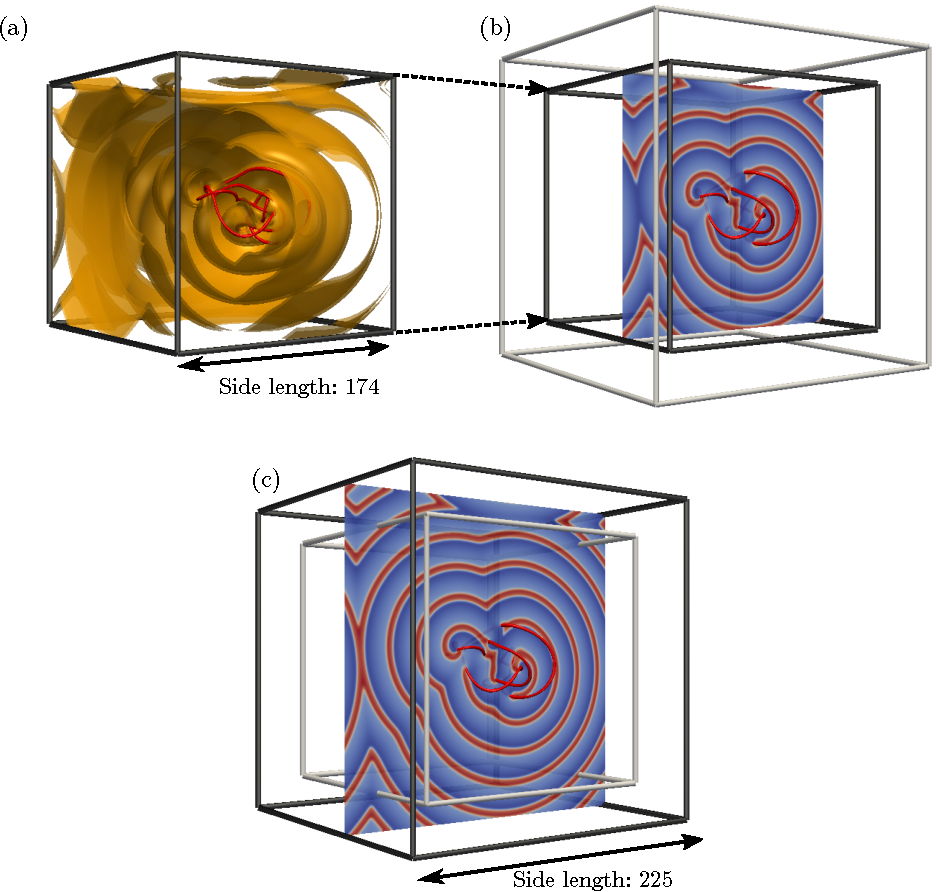
\includegraphics[keepaspectration, width=0.99\linewidth ]{\FitzHughNagumoFigures/BoxSizeInvariance/BoxSizeInvariance.pdf}
    \caption[A typical simulation of knotted vortices in the FitzHugh-Nagumo model.]{\label{fig:TypicalSimulation} (a) A snapshot of a typical simulation, here of the $7_2$ knot $T=2420$ after initialisation, demonstrating the structure of the wavefield in a periodic simulation box. The level set $|{\bf B}|=0.4$ (red tube) marks the vortex filament, and contours of $ u = 1.6$ mark the location of propagating wavefronts (orange paired surfaces). The near quarter of the wavefronts are clipped to reveal their inner structure. The wavefronts have a complex topology at lengths comparable to that of the vortex, but away from it take the form of simple concentric shells. (b, c) Snapshots of the same $7_2$ knot evolution simulated in boxes of different sizes. (b) replicates (a), with a cross section through the $u$ wavefield shown (wavefronts in red). (c) shows the corresponding knotted vortex and wavefield from the larger box (dark grey simulation box corresponds to cross section shown). Differences in the wavefields are localised to the boundary of the smaller simulation box, ensuring we are indeed capturing bulk dynamics. As expected, the knot loci themselves are identical.}
\end{figure}
Stacking two-dimensional spiral vortices one obtains the simplest example of a vortex filament, one with a straight geometry from which emanates a quasi-two-dimensional `scroll wave'~\citep{Winfree1983}. More generally, the vortex filament is a tubular structure with arbitrary geometry, normal cross sections of which resemble spiral vortices whose phase is allowed to vary longitudinally. (In fact even this picture is an idealisation; waves emanating from other sections of the filament can disrupt this local spiral wave structure.) Various operational definitions to extract a one-dimensional curve from this tubular structure have been proposed~\citep{Winfree1990,Henze1993,Dowle1997}. Here we follow~\citep{Sutcliffe2003,Maucher2016,Maucher2017,Maucher2018,Maucher2019} and first compute the intermediate quantity
\begin{equation}
\label{eq:ucrossv}
\mathbf{B} = \nabla u \times \nabla v.
\end{equation}
$|\mathbf{B}|$ measures the deviation of $u$ and $v$ contours from colinearity --- it is zero for a planar wave, and only attains substantial nonzero value along the vortex filament. Contours of $|\mathbf{B}|$ thus take the form of tubes. For example, figure~\ref{fig:TypicalSimulation} tracks the vortex filament by showing the level set $|{\bf B}| = 0.4$ in red. To extract a one-dimensional curve from such a tube, we first note that $\bf B$ orients the tube. Stepping along the tube in the direction given by this orientation, we connect maximal values of $|\mathbf{B}|$ in cross sections taken through it, resampling if necessary to give equidistant steps; a similar extraction procedure is detailed in~\citep{Winfree1990}. This raw curve is then smoothed to remove modes of frequencies comparable to $\lambda$, giving a smoothed curve from which we may compute curvatures and torsions via finite difference. (The choice of lengthscale for filtering is motivated by the observation that the most highly curved stable filament observed, a stable round unknot~\citep{Courtemanche1990}, has a circumference comparable to $\lambda$.) Typically we will use the term `filament' to emphasise the one-dimensional curve defined above, and `vortex' when we wish to discuss the full tubular stack of spiral waves surrounding this curve. This definition (and indeed other `instantaneous' definitions~\citep{Dowle1997}) gives rise to small amplitude oscillations in the geometry of the filament at period $\sim T_0$ which carry through to derived quantities such as knot length. We shall examine the spectrum of these oscillations in detail in \S\ref{sec:StableKnots}, but in subsequent plots showing length evolution we filter them out for clarity. 

As discussed above, vortex phase varies along the filament, framing our one-dimensional curve, and the twist of this framing may in principle affect both filament motion and vortex rotation period. We track it by computing $\frac{\nabla u}{|\nabla u|}$ along the filament and then smoothing as above. 

\subsection{Initialising a knotted vortex field}
\label{subsec:WavefieldInitialisation}

To initialise an arbitrary knotted vortex for simulation we adopt the basic strategy of~\citep{Sutcliffe2003,Maucher2016} in which a phase field $\phi( {\bf x}) \in \mathbb{S}^1$, ${\bf x} \in \mathbb{R}^3\setminus K$, is constructed which contains a phase singularity with the geometry of some desired vortex knot $K$. Thereafter, the winding of $\phi$ around the specified knotted phase singularity is translated into the winding of $(u,v)$ around the excitation-recovery loop of the FitzHugh-Nagumo model as one encircles the vortex filament via the map $ (u,v) = (2 \cos \phi - 0.4, \sin \phi - 0.4)$.

To construct a phase field $\phi$ containing a singularity along a given curve $K$, we first compute the solid angle function $\omega$ about $K$ using \eqref{eq:OurSolidAngle1} from \S\ref{sec:CurveIsotopies}~\citep{Binysh2018} 
\begin{equation}
    \omega({\bf x}) = \int_{K} \frac{{\bf n}_\infty \times {\bf n} \cdot \mathrm{d}{\bf n}}{1 + {\bf n} \cdot {\bf n}_\infty} \quad \mathrm{mod}\;4\pi,
    \label{eq:SolidAngle}
\end{equation}
where for ${\bf y} \in K$, ${\bf n} := \frac{{\bf y} - {\bf x}}{|{\bf y}-\bf{x}|}$ is the projection of $K$ onto a unit sphere centred on $\bf x$ and ${\bf n}_\infty$ is an arbitrary unit vector. For a discussion of this integral and its numerical properties, including its singular behaviour about points ${\bf x}$ such that ${\bf n} \cdot {\bf n}_\infty = -1$, see~\S\ref{sec:NumericalImplementation} \citep{Binysh2018}. 
    

The solid angle contains the necessary phase singularity along $K$, and for the simulations discussed in this chapter we use it for initialisation directly by setting $\phi = \omega/2$. We emphasise that, although $\omega$ contains the correct topology to be used as an initialisation condition, the structure of $\omega$ about $K$ does not mirror that of a typical $(u,v)$ wavefield, which consists of a series of approximately equispaced wavefronts radiating outwards from the vortex filament (figure \ref{fig:TypicalSimulation}) --- after $\sim T_0$, $\phi = \arctan \left(2(v+0.4)/(u+0.4)\right)$ no longer resembles $\omega$. Further, this methodology does not give control over the initial twist distribution along the filament, which is set by the intersection of the level set $\omega=0$ with $K$, the solid angle framing of $K$ discussed in~\S\ref{sec:LocalStructure}~\citep{Binysh2018}. We may control both of these features by modifying $\phi$ as
    
\begin{equation}
\phi({\bf x}) = k_0 d({\bf x}) + \frac{1}{2} \omega({\bf x}), 
\label{eq:WavefieldInitialisation}
\end{equation}
where $k_0 := 2\pi / \lambda_0$ is the spiral wavenumber and $d({\bf x}):= \mathrm{min}_{{\bf y} \in K} |{\bf y}- {\bf x}|$ is the minimal distance from ${\bf x}$ to $K$. $k_0 d({\bf x})$ increases linearly with distance from the curve, giving a periodic modulation of $\phi$ and hence $(u,v)$ with distance. As an example, figure~\ref{fig:WavefieldInitialisation}(a) shows the wavefield generated using~\eqref{eq:WavefieldInitialisation} when $K$ is a trefoil knot. The intersection of the level set $\phi=0$ with $K$, and hence the initial twist distribution, may be controlled by including an offset in the definition of $d({\bf x})$ which varies along $K$. An example of such a modulation, and how it alters the wavefield, is shown in figure~\ref{fig:WavefieldInitialisation}(b). Given, for example, the importance of twist distribution on both rotation frequency and the sproing instability as discussed above (and further explored in this chapter), such control is desirable for future work.

Initialisation geometries for the knots considered here were constructed from those found in \emph{KnotPlot}~\citep{KnotPlot}, which in turn are based on Rolfsen's knot table. In the absence of existing work on high crossing number knots in the FitzHugh-Nagumo model, there is no compelling reason to choose one set of initialisation geometries over another; for example, an alternative choice would be to use configurations of ideal ropelength~\citep{Cantarella2011,Kleckner2016,Maucher2017}. We use Rolfsen's configurations as, with the exception of the torus knots (whose evolutions we will compare to existing results~\citep{Maucher2017}) the geometries do not possess any symmetries. If strands of the knot are initialised closer to one another than the vortex radius $\lambda_0 /2\pi$, reconnections may occur in the first $\Delta T \approx T_0$ of simulation, before the wavefield about the knot is established~\citep{Maucher2016}. To ensure this does not occur, given an initialisation geometry $K$ we scale isotropically such that the longest side of $K$'s bounding box occupies $80\%$ of the simulation box size. As the simulation box is $O(50)$ times the size of the vortex radius, this ensures reconnections do not occur during initialisation. 

\begin{figure}[htbp]
\centering
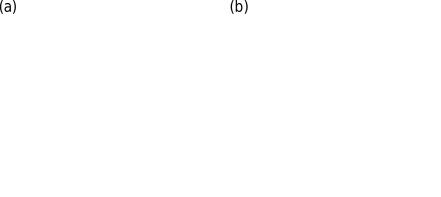
\includegraphics[keepaspectration, width=0.85\linewidth ]{\FitzHughNagumoFigures/WavefieldInitialisation/WavefieldInitialisation}
  \caption[Initialising a wavefield around a trefoil vortex.]{Wavefield initialisation about a trefoil knot vortex filament (red curve) using~\eqref{eq:WavefieldInitialisation}, with the level set $\phi = 0 $ shown in orange. The near half of the level set is clipped to reveal its inner structure. In (a) the definition of $d({\bf x})$ in~\eqref{eq:WavefieldInitialisation} is simply minimal distance to the filament. In (b) it is modified by a threefold symmetric sinusoid along the trefoil, $d({\bf x})= \mathrm{min}_{{\bf y} \in K} |{\bf y}- {\bf x}| + \frac{L}{5}\sin(3s)$ where $s$ is arclength (as measured from the intersection of the trefoil with the $xy$-plane) and $L$ is total trefoil length, effectively adjusting the solid angle framing and local twist rate of the vortex filament.}
\label{fig:WavefieldInitialisation}
\end{figure}


\section{\label{sec:UnstableKnots}Unstable Knots}

\begin{figure}[htbp]
\centering
    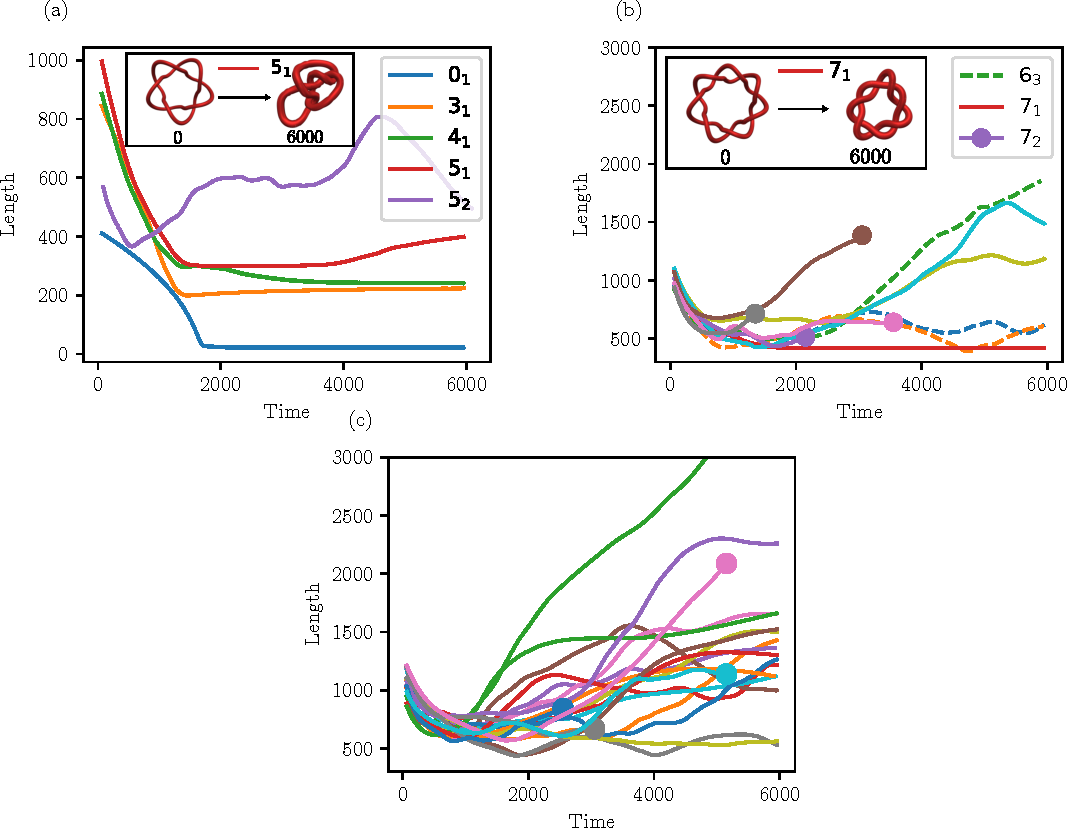
\includegraphics[width=0.99\linewidth]{\FitzHughNagumoFigures/UnstableKnotsLength/UnstableKnotsLength_annotated.pdf}
    \caption[Length evolution of knotted vortices up to and including crossing number eight.]{ Length evolution of knotted vortices up to and including crossing number $N=8$, with reconnection events indicated by curves which terminate early with a circular marker. Knots included in the legend are further discussed in the text. Note the difference in scale between the first and subsequent panels. (a) $N\leq5$. (b) $N=6$ (dotted lines) and $N=7$ (solid lines). (c) $N=8$. The unknot ($0_1$), trefoil ($3_1$) and figure eight ($4_1$) settle to a stable length and fixed geometry (see section \ref{sec:StableKnots}). However, beyond this, generic behaviour is an initial period of contraction, followed by length increase over longer timescales. Insets show the geometries resulting from the destabilisation of the initially symmetric $5_1$ and $7_1$ torus knots.} 
\label{fig:UnstableKnotsLength}
\end{figure}

\begin{figure}[htbp]
\centering
    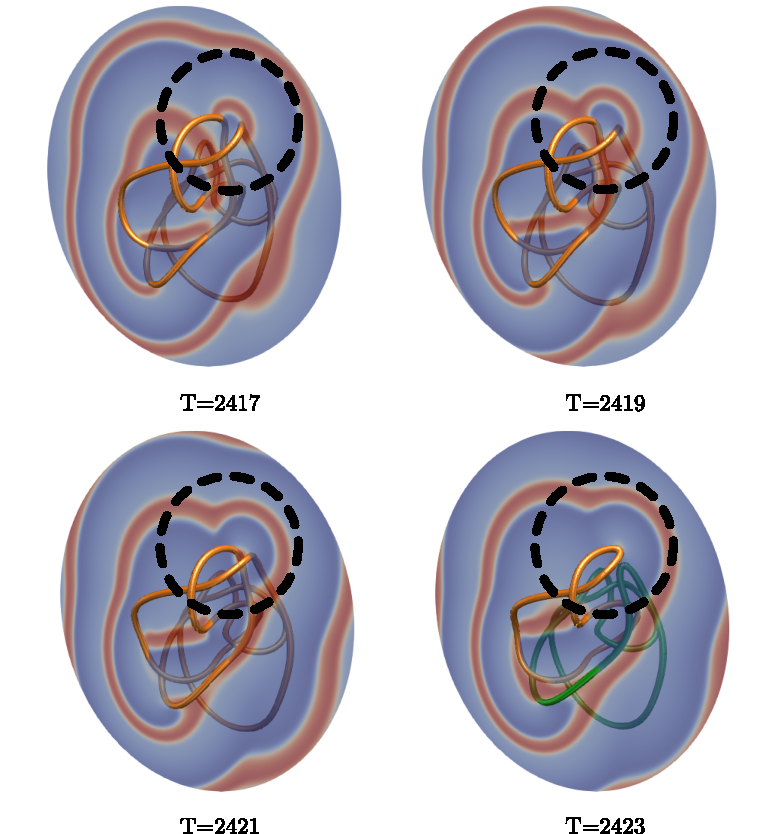
\includegraphics[width=0.99\linewidth]{\FitzHughNagumoFigures/Reconnections/ReconnectionsFigure.pdf}
    \caption[Reconnection of the $7_2$ knot.]{Reconnection of the $7_2$ knot at $T=2423$ (orange curve, then orange and green curves after reconnection event) shown in $\Delta T = 2$ increments. A pair of anti-parallel strands (circled in black) interact, generating a wavefield locally similar to that of the stable unknot; shown is the value of $u$ in a cross section through the knot, with high $u$ value coloured red. The wavefield from the remainder of the knotted filament, shown entering the circled region at $T=2417$, impinges upon these strands causing them to destabilise and reconnect. Note that the wavefield at $T=2420$ is also shown in figure~\ref{fig:TypicalSimulation}.}
\label{fig:Reconnections}
\end{figure}

Fascinating recent numerical experiments on the evolution of unknots initialised in complex geometries showed that the FitzHugh-Nagumo dynamics is capable of simplifying an initially tangled unknot to a unique circular curve, without strand crossings~\citep{Maucher2016}. These intriguing examples, coupled with two further instances of simplification in the case of the trefoil~\citep{Sutcliffe2003}, as well as some indirect evidence of the same behaviour for the Hopf link~\citep{Maucher2019} (and a series of preliminary results on various links in~\citep{Henze1993}), naturally invite the speculation that such simplification is generic to any knot. To investigate the dynamics of a generic knotted filament, and establish whether this is indeed the case, in figure~\ref{fig:UnstableKnotsLength} we show a survey of the length evolution of all knots up to and including crossing number $N=8$, with particular curves that we discuss further highlighted in the legend. Excluding chiral variants, there are thirty-six such knots. 

Initial behaviour across all knots is contraction; this behaviour is purely a result of curve geometry, reflecting an effective positive line tension for filaments well separated from any interactions~\citep{Biktashev1994}. Our curves are initialised with their strands separated by several vortex radii. Over the first few vortex rotation periods the wavefield establishes itself around the vortex filament (over such a timescale the filament may be considered stationary) with the resulting collision interface disjoint from the filament itself. Thereafter each segment of the filament initially moves effectively in isolation from its neighbours. 

Over longer timescales, however, we find that this initial contraction does not generically lead filaments to settle to a canonical form or a fixed length, and further that their topology is not always preserved. We observe reconnection events in eight of the thirty-six cases, indicated by those curves terminating in circular markers in figure~\ref{fig:UnstableKnotsLength}. The first of these occurs at $N=7$, with four of the seven $N=7$ knots and four of the twenty-one $N=8$ knots exhibiting reconnections.

Figure~\ref{fig:Reconnections} shows the reconnection event in the $7_2$ knot occurring at $T=2423$ in $\Delta T=2$ increments, with the region where the reconnection occurs circled in black. A pair of neighbouring anti-parallel segments are directly impacted by waves emanating from the rest of the knotted filament, causing them to destabilise and reconnect --- the same wave slapping mechanism responsible for the annihilation of a small unknot by a larger one observed in~\citep{Maucher2018}. In cross section, the wavefield generated by the anti-parallel segments (that section of the wavefield ending at the circled anti-parallel segments in the $T=2417$ panel of figure 4) locally resembles that of a stable unknot, or indeed of a pair of oppositely signed two-dimensional vortices~\citep{Courtemanche1990}. However this stable structure is additionally impinged upon by the wavefield of the rest of the knot (shown entering the circled region at $T=2417$). It has previously been noted that the rotation period of a stable unknot is 14\% greater than $T_0$~\citep{Maucher2018}, and as such the stable unknot is vulnerable to wave-slapping induced annihilation by a wavetrain of period $T_0$, with the frequency difference leading to motion of the collision interface towards the stable unknot at speed $c\Delta T/2T_0$, where $c$ is the wavespeed in the medium~\citep{Courtemanche1990,WinfreeChapter}, until the interface directly impinges upon the unknot --- this process is shown schematically in figure~\ref{fig:WaveSlapping}, and a simulation of it may be found in~\citep{Courtemanche1990}. This same argument applies to the anti-parallel segments discussed here, but the resulting topological change is reconnection. In addition to the similarity of the wavefields between the coaxial unknots of~\citep{Maucher2018} and the situation discussed here, the relative filament motion is also the same; in both cases, the perturbed filaments are drifting away from the impinging wavefield when topological change occurs. This geometric detail is important, as the velocity of a stable unknot ($0.3$~\citep{Maucher2018}) is a substantial fraction of the wavespeed in the medium ($1.9$) and as such Doppler shift may compensate for reduced unknot frequency. For the geometry here, however, the two effects can only compound one another. 
\begin{figure}[htbp]
    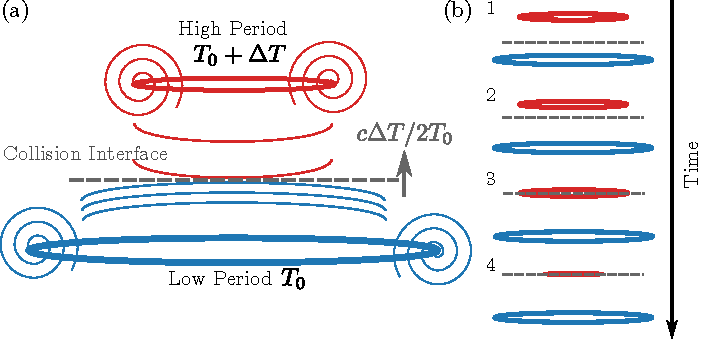
\includegraphics[keepaspectration, width=0.99\linewidth ]{\FitzHughNagumoFigures/WaveSlapping/WaveSlapping.pdf}
    \caption[Wave slapping]{\label{fig:WaveSlapping} A schematic of wave slapping between a pair of unknots. (a) A large unknot (blue) emits waves of activity with speed $c$ at a period $T_0$, which travel towards a smaller unknot (red), which emits at $T_0 + \Delta T$. The locus where the two wavetrains meet and annihilate is called the collision interface (grey). The difference in emission frequencies causes this interface to move at speed $c\Delta T/2T_0$. (b) The collision interface moves towards the smaller unknot (1, 2) until directly impinging upon it (3). This causes the smaller unknot to destabilise (4).}
\end{figure}

Topology changes previously reported in the literature have primarily occurred at simulation boundaries~\citep{Maucher2017, Maucher2019}, and one might be concerned that this reconnection is also an artefact of a finite simulation box. The snapshot of a $7_2$ simulation at $T=2420$ shown in figure~\ref{fig:TypicalSimulation} was taken from the same data shown in figures~\ref{fig:UnstableKnotsLength}, \ref{fig:Reconnections}, and was chosen specifically to emphasise that this is not the case. Enlarging the simulation box to side length $225$ as shown in figure~\ref{fig:TypicalSimulation} yields identical knot evolution, including the reconnection event.

Although we have focused the above discussion on the reconnection in the $7_2$ knot, analogous findings hold for the other cases. A detailed understanding of the wavefield evolution leading to such reconnections, and why they are seen here only for $N>5$, is lacking (we shall see examples of similar wavefield induced effects for small $N$ in \S \ref{sec:StableKnots}), but as $N$ increases one generically expects a more complex wavefield surrounding the knot as strands become closely packed over one another. As such, we lose the ability to picture segments of the knot as isolated, or even as interacting solely with a unique `nearest neighbour' region, but instead must think of them analogously to the vortex ring buffeted by external waves.

Even in the absence of reconnections, we only see stable states for the unknot, trefoil and figure eight knots; we shall discuss the robustness and detailed geometry of these states in \S \ref{sec:StableKnots}. For $N>4$ knots do not simplify. After the initial relatively rapid contraction, we generically see expansion over a much longer timescale of order several hundred vortex rotation periods followed by periods of irregular evolution including possible further expansion. Although the broad trend is to faster expansion at higher crossing number, the variability of behaviour between knots of the same crossing number suggests that initialisation geometry is just as important in determining long time evolution. In particular, we note the discrepancy between the behaviour of a typical knot with no initial symmetry and a torus knot initialised with high symmetry. Although a typical knot shows length increase by time $T\approx2000$, for the $5_1$ knot shown in figure~\ref{fig:UnstableKnotsLength} this increase is only visible by $T\approx4000$, and is not evident for the $7_1$ even by $T\approx6000$, although the inset curve geometries demonstrate the knot has indeed destabilised (that such destabilisation occurs, but only after long time simulations, clearly demonstrates the necessity of simulating for many hundreds of rotation periods before drawing conclusions about the dynamics of this system). In the next section, we shall investigate the mechanisms of both the dramatic length increases seen in a generic knot, and of the deviation of the torus knots away from initialisations of high symmetry. 
\begin{figure*}[htbp]
\centering
    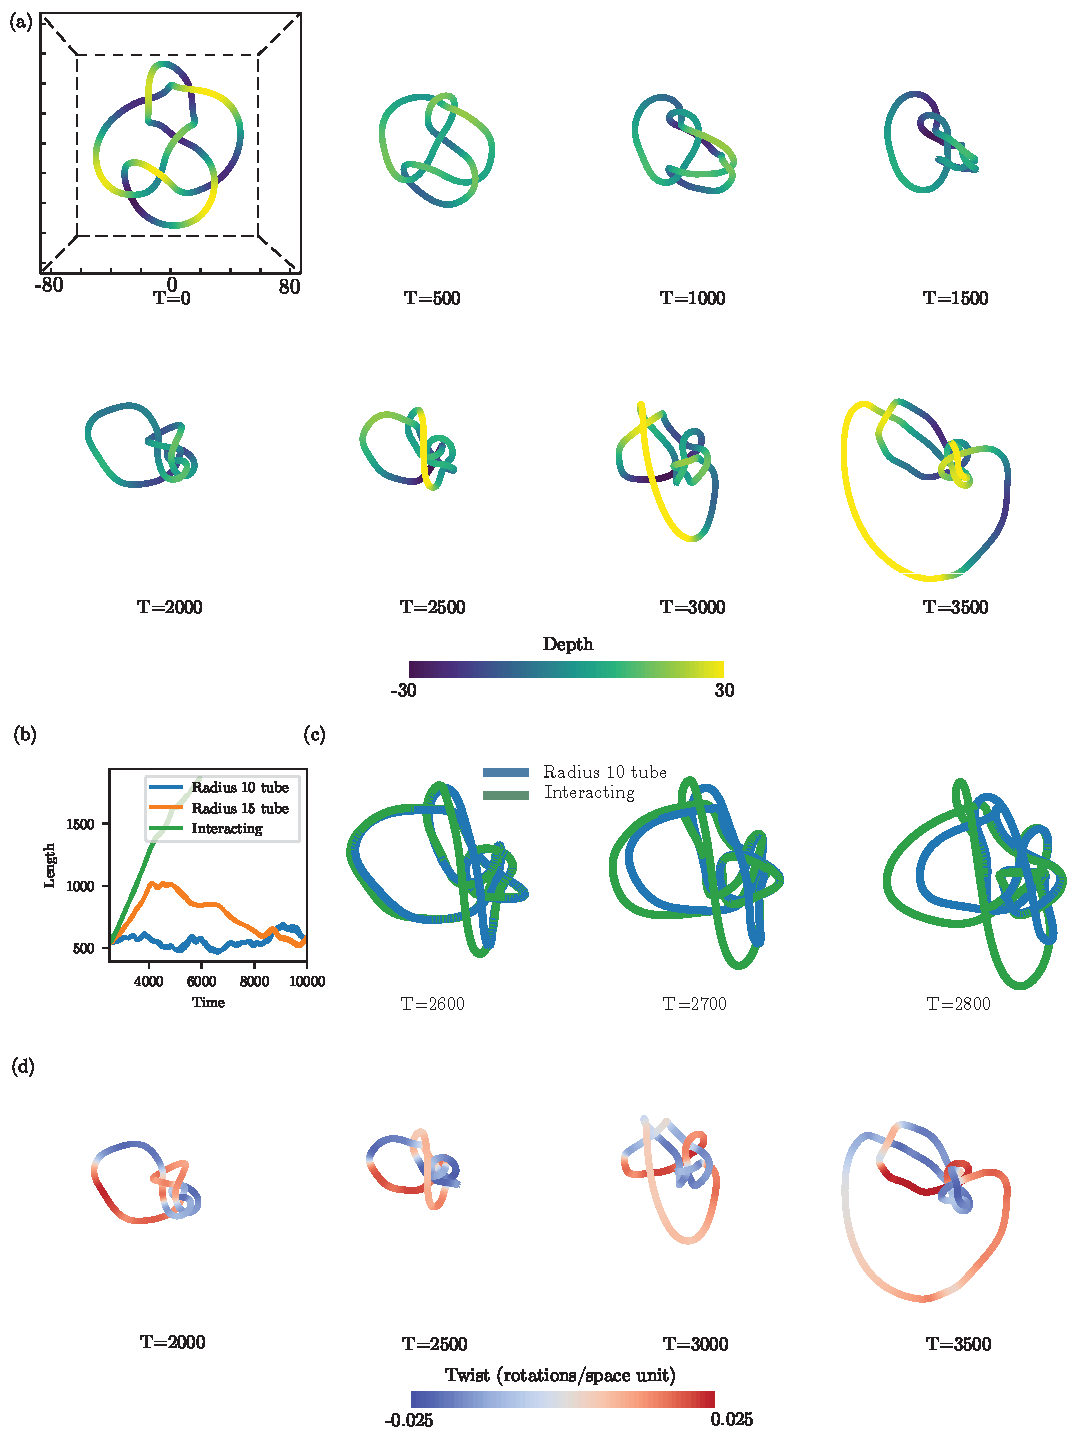
\includegraphics[width=\textwidth]{\FitzHughNagumoFigures/63evolution/6_3}
\end{figure*}
\subsection{The mechanism of vortex knot length increase}
\label{subsec:Mechanism}
\begin{figure*}[hbtp]
    \caption[Dynamics of the $6_3$ knot.]{(overpage) Dynamics of the $6_3$ knot. (a) From $T=0$ to $T=2000$ the knot contracts and flattens, behaviour caused by the intrinsic curvature driven dynamics of an isolated filament mimicking a line tension. From $T=2000$ onwards length increases, with a single arm of the knot rapidly expanding outwards from an otherwise tightly packed core. (b) Comparison of the length evolution of the fully interacting $6_3$ vortex filament at $T=2000$ (green) to a copy encased in a `glass tube' of radius 10 (blue) or 15 (orange). With long-ranged interactions removed, the knot does not expand, but rather settles to a length of $\sim 400$ -- $600$. (c) Initial divergence in geometries between the interacting $6_3$ knot (green curve) and the radius $10$ tubed one (blue curve). Divergence does not occur globally, but is localised to two distinct expanding segments outside the lengthscale defined by the tube. (d) Distribution of filament twist during knot expansion. The expanding arm of the knot has twist values well below the $0.024$ rotations per space unit threshold for the sproing instability, and is less highly twisted than other, non-expanding, segments of the knot, ruling out this instability as the cause of length increase.}
\label{fig:63evolution} 
\end{figure*}
Exploring the knot geometries corresponding to the generic length increases seen in figure~\ref{fig:UnstableKnotsLength} one finds that, despite the variety of behaviour across knots, the increase occurs via a common mechanism in which isolated strands of the knot rapidly expand outwards from a tightly packed core region forming the rest of the knot. We illustrate this behaviour for the example of the $6_3$ knot in figure~\ref{fig:63evolution}(a). The same wave slapping mechanism driving reconnection events has also been proposed as a non-local mechanism for persistent knot length increase; in this context when the collision interface intersects a section of the knot, wave-vortex interactions drive that section outwards~\citep{WinfreeChapter,Sutcliffe2003}. The interaction does not have an intrinsic lengthscale, as waves in the medium do not decay. Instead, its range depends upon the geometry of the knot and the accompanying collision interface. For the $6_3$ knot shown in figure~\ref{fig:63evolution} one may verify that this surface intersects the expanding arm, suggesting that wave slapping may be at play. 

Given the potential importance of this mechanism, we would like to establish that it is really driving knot expansion, rather than simply being correlated with it. To do so, we investigate the effects of abruptly removing long-ranged interactions entirely, by numerically encasing the filament in a `glass tube' of moderate radius which moves with the filament and fuses when two knot segments approach one another~\citep{Winfree1983b}. With this construction short-range inter-filament repulsion, and geometry (including twist) mediated filament motion are preserved but long-ranged interactions are cut out. Using it, we may compare the evolution of a filament both with and without long-range interactions. A suitable radius for the tube is suggested by previous estimates of vortex radius in the literature, as well as the naive estimate $\lambda_0/2 \pi \approx 3.4$:~\citep{Courtemanche1990} directly measures a stable vortex ring radius of $4.8$, suggesting a vortex radius of $\sim~5$, and~\citep{Maucher2017} estimates a radius of $5.9$ by matching ideal ropelength~\citep{Cantarella2011} and measured trefoil lengths. To implement this construction numerically we simulate only within a tube of lattice points about the filament (the filament itself being constructed as in \S\ref{sec:Methodology}). In principle the details of the boundary conditions between the vortex and tube must be considered, however we have found that provided we use a tube radius above the vortex size estimates above, such details do not alter the geometry driven motion of the vortex, a reflection of its localised nature. This observation allows us to sidestep a sophisticated finite-element scheme (the spectral method discussed in \S~\ref{subsec:Simulation} only being valid for a periodic box), and instead simply use a finite difference method, with $(u,v)$ values for points outside of the tube set to their fixed point values $(-1.03,-0.66)$. The tube must move with the vortex, however we note that this need only happen on the (slow) timescale of vortex motion; we may allow motion in a fixed tube for a time $O(T_0)$, after which the tube is recentred around the vortex. The points brought into the tube at its boundary during this procedure are again set to fixed point $(u,v)$ values. In practice we typically use a conservative tube radius of $\sim 10$ with gridspacing $\Delta x = 0.5$ and timestep $\Delta t = 0.01$, with a finite difference scheme in which the Laplacian is computed using a seven point stencil and both reaction and diffusion terms are evolved using fourth order Runge-Kutta timestepping. The timestep above is chosen as it gives results identical to those of the spectral method using $\Delta t = 0.1$ when measuring the two-dimensional spiral vortex period. 

Figure~\ref{fig:63evolution}(b) contrasts the length evolution of the fully interacting $6_3$ knot with a copy of it encased in the tube, with initial conditions for both taken at $T=2500$, midway through knot expansion. Upon removing long-ranged interactions we no longer see a dramatic increase in knot length. Instead, the length of the tubed knot stabilises at $\sim 400- 600$. The details of this stabilisation vary depending on the radius of the tube, but the final lengths obtained are approximately the same across radii. Using the core size estimate of~\citep{Maucher2017}, the ideal ropelength of the $6_3$ knot is $340$~\citep{Cantarella2011}, and thus the tubed knot is relatively tightly packed. Over longer timescales ($\Delta T=8000$ shown for the radius $10$ tube of figure~\ref{fig:63evolution}(b)) the tubed $6_3$ does not reach a fixed geometry, but rather undergoes a compact tumbling motion, as the binormal component of filament motion causes segments of the knot to work over one another, though without further substantial length change. In figure~\ref{fig:63evolution}(c) we explore the initial divergence in geometry between the fully interacting and tubed knots. We see that it does not occur globally, but is localised to distinct expanding segments of the interacting $6_3$ which lie separate to the knot core region and are responsible for global length increase; these same segments are those which intersect the collision interface. Within the core region, segments of the filament are packed closer than the spatial cutoff we have defined, and there is no immediate divergence between the interacting and tubed knots. By contrast, removing long-range interactions allows distant segments of the tubed knot to evolve under their intrinsic dynamics, unaffected by wave-vortex interactions, and so shrink towards the core region. Thus a wave slapping mechanism accounts for global changes in knot length and also for the geometry of where they occur. 

In local geometric models of filament motion a mechanism by which filament length may stabilise or increase, despite an effective positive line tension, is via the `sproing' instability~\citep{WinfreeChapter} in which, above some critical local twist threshold, an initially straight filament expands into a helix --- for the FitzHugh-Nagumo model with the parameter values used here,~\citep{Henze1993} reports this threshold at 0.024 rotations per space unit for a straight filament. This instability has been proposed to account for the halting of links at lengths greater than hard core repulsion on the scale of the vortex radius would suggest~\citep{WinfreeChapter}, and for the destabilisation of symmetric torus knots~\citep{Maucher2017}. We may rule out sproing as a driver of the dramatic length increases seen in generic knots by noting that, as a local geometric mechanism, its effects were present in the tubed knot discussed above. For further confirmation, we may also examine the twist distribution along the fully interacting filament during knot expansion. Figure~\ref{fig:63evolution}(d) shows this distribution for the $6_3$ knot; we see that the expanding arm of the filament consistently has twist values well below the sproing threshold and, further, that other sections of the knot are more highly twisted, yet do not show the same length increase. In fact, twist values along the entirety of the knot are consistently below the sproing threshold, an observation also made for the early short time simulations of~\citep{Henze1993,WinfreeChapter}. 

Although not a driver of generic knot length increase, this last observation suggests that the sproing threshold may still have dynamical importance as a stabiliser against curvature induced length decrease, or play a role in the destabilisation of symmetric torus knots. In figure \ref{fig:TorusDestabilisation} we study the destabilisation of the $5_1$ torus knot, originally presented in figure \ref{fig:UnstableKnotsLength}, in more detail. Figure \ref{fig:TorusDestabilisation}(a) shows the evolution of a measure of the asymmetry of the knot, defined by taking the power spectrum of the knot's curvature as a function of arclength, and computing the fraction of the power in modes which do not respect the underlying symmetry (fivefold in this case). Alongside it we show the evolution of both the maximal twist, expressed as a fraction of the $0.024$ rotations per space unit sproing threshold discussed above, and the fraction of the arclength of the $5_1$ which attains a twist greater than $90\%$ of this threshold. We first note that the order of events is broadly consistent with sproing threshold playing a role in the dynamics. After an initial period in which the knot flattens and the twist remains roughly constant, maximal twist increases until it attains the sproing threshold, thereafter remaining constant; this threshold is attained as the length of the $5_1$ stabilises. However, it is several hundred rotation periods before we see the subsequent loss of symmetry. This timescale suggests that it is not the case that the knot hits the sproing threshold, and then destabilises;~\citep{Henze1993} notes that the timescale for sproinging to occur is typically only a few rotation periods. Furthermore the geometry of the destabilisation is inconsistent with sproing instability. In figure~\ref{fig:TorusDestabilisation}(b) we show the knot as it destabilises, coloured by twist. We fail to see helical sproinging along the highly twisted segments of the knot; instead the whole form collapses to a twofold symmetric shape. A similar deformation is seen in the $7_1$ (see inset of figure \ref{fig:UnstableKnotsLength}) and has been noted in early simulations of initially symmetric triply-linked rings~\citep{Henze1993}, where its cause was attributed to an interplay between the sproing threshold and inter-filament interactions. Overall, then, it appears the sproing threshold acts to halt knot shrinkage, but that subsequent destabilisation cannot be directly attributed to the sproing instability. 

\begin{figure}[htbp]
\centering
    \includegraphics[width=0.7\linewidth]{\FitzHughNagumoFigures/TorusDestabilisation/TorusDestabilisation.pdf}
    \caption[The role of the sproing instability in knot destabilisation.]{ The role of the sproing instability in the destabilisation of the $5_1$ torus knot. (a) shows the (normalised) length evolution of the $5_1$, alongside a measure of its asymmetry. Shown also is the maximum absolute twist along the knot as a fraction of the 0.024 rotations per space unit sproing threshold, and the fraction of arclength which attains 90\% of this threshold. The twist threshold is reached as knot length plateaus, but no sproinging instability is observed; instead the knot gradually destabilises over several hundred rotation periods. (b) shows the geometry of the knot destabilisation, coloured by twist. Rather than a helical instability developing in regions of high twist, the whole knot transitions to a twofold symmetric form.}
\label{fig:TorusDestabilisation}
\end{figure}

\section{\label{sec:StableKnots}Stable Knots}
\begin{figure}[htbp]
    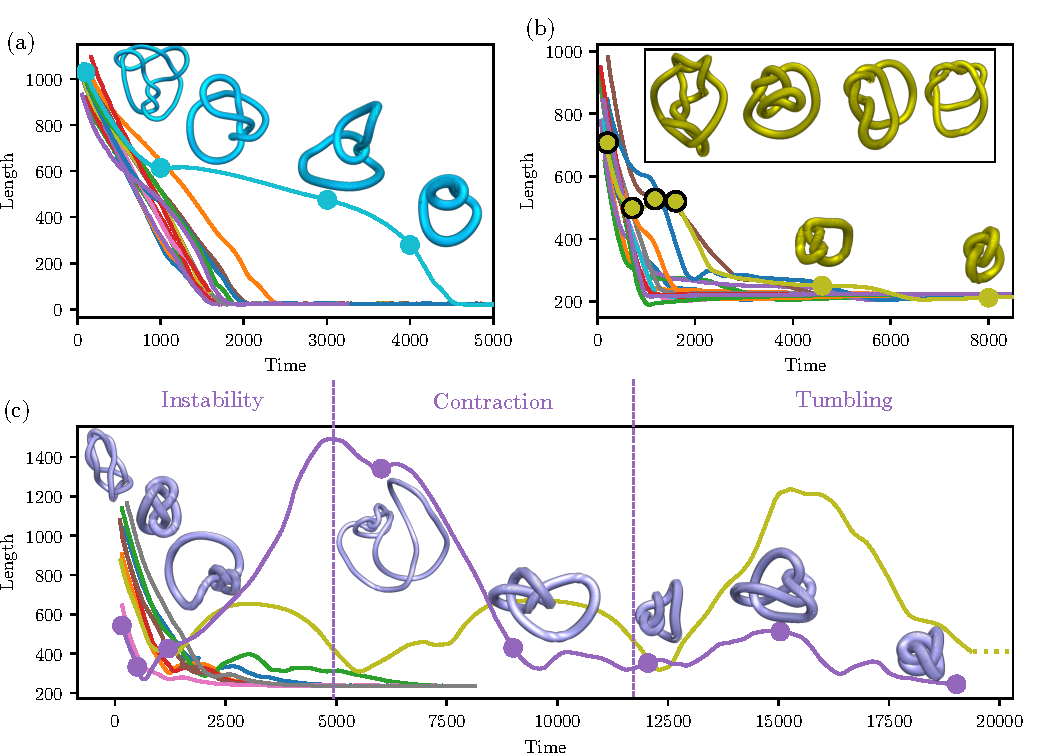
\includegraphics[width=0.99\linewidth]{\FitzHughNagumoFigures/SecretKnots/SecretKnots.pdf}
    \caption[Untangling dynamics.]{ Untangling dynamics of the (a) 18 unknots, (b) 17 trefoils and (c) 9 figure eight knots formed by performing single strand crossings on the higher crossing number knot geometries of \S \ref{sec:UnstableKnots}. (a) All unknots simplify to a unique round geometry without reconnection events. Length decrease is monotonic, however there is some variation; the geometry of one particularly slow decay is shown in the inset, displayed at times indicated by the solid markers. (b) All trefoil geometries simplify to a unique stable state, however there is greater variation across decays than for the unknots, with periods where knot length actively increases (boxed inset, circled markers). (c) Of the $9$ tangled figure eights simulated, $7$ settle rapidly to a stable state. However, over $T=20000$ one example fails to converge and another converges only after going through prolonged periods of length increase, contraction and irregular `tumbling' dynamics.} 
\label{fig:SecretFourOneLength}
\end{figure}

In \S \ref{sec:UnstableKnots} we showed that the speculation that a generic knotted vortex might simplify to a canonical form --- a speculation previously evidenced by promising `untangling' results for the unknot~\citep{Maucher2016} and a few further examples of simplification in low crossing number knots and links~\citep{Sutcliffe2003,Maucher2019} --- is not borne out for $N>4$. In the search for stable knots, recent numerical experiments found that knots and links could be stabilised through proximity to a no-flux boundary~\citep{Sutcliffe2003,Maucher2017}. Primarily the examples shown were for torus knots and links, although the figure eight knot and Borromean rings were also briefly given as non-torus examples. In contrast to the untangling of unknots, these boundary stabilised states of more complex vortices were not established to be `basins of attraction' for generic initial geometries, but rather were obtained from highly symmetric initial vortex line geometries. In \S \ref{sec:UnstableKnots} we also saw that in the case of torus knots more complex than the trefoil such states are not stable in our bulk simulations. By contrast, for the stability of the trefoil and figure eight knots we now show that a much stronger statement than has been made previously is true: in the bulk, a generic trefoil or figure eight simplifies to a canonical form, analogously to the unknot. The states are the same as those found in the survey of figure \ref{fig:UnstableKnotsLength} and also appear to be the same as those found near a reflecting boundary. In addition, we strengthen the results of~\citep{Maucher2016} and demonstrate them to be independent of a no-flux boundary by testing the bulk untangling dynamics of the unknot with a far greater variety of initial conditions than has been used previously.

All knots may be converted into the unknot by performing strand crossings. The minimal number of strand crossings needed to convert a knot into the unknot is called its unknotting number. Of the knots with $N\leq8$ there are $18$ with unknotting number $1$; that is, they can be converted to the unknot by a single strand crossing. By analogous single strand crossings one can also target the trefoil or figure eight knots: for $N\leq8$ there are $17$ that convert to the trefoil and $9$ to the figure eight under a single strand crossing. Beginning with the knot geometries of \S \ref{sec:UnstableKnots}, we use these crossings to provide an assortment of initial tangled geometries for unknots, trefoils, and figure eights, and study their evolution. Figure~\ref{fig:SecretFourOneLength}(a) summarises the results of these simulations for the tangled unknots. We find in all cases that the initially tangled vortex transforms to a unique stable ring and that the dynamics does not involve any reconnections. The typical dynamics is an approximately constant rate of length contraction, although this is not rigorous and there is some variation. In particular, in one example (obtained from the $8_{11}$ knot) there is a substantial period of pause where length decreases much more slowly than is seen on average; snapshots of the geometric evolution of this curve are shown as insets. 

Figures~\ref{fig:SecretFourOneLength}(b),(c) show results for the trefoil and figure eight knots. As with the unknot, for the trefoils we see simplification without reconnection to a unique steady state, although there are perhaps more examples showing periods where the length is not decreasing; one such is illustrated by the inset figures. However, for the figure eights the dynamics is rather more complicated; $7$ of the $9$ initialisations rapidly converge to a unique stable state, but $2$ show prolonged periods of length increase as well as of contraction, with one of them failing to converge over the times simulated. In the example highlighted in figure~\ref{fig:SecretFourOneLength}(c), we see that the initial period of expansion is due to a single arm of the knot rapidly expanding outwards from an otherwise tightly packed core, caused by the same wave slapping as described in \S\ref{sec:UnstableKnots}. This expansion continues for many hundreds of rotation periods and results in a total increase of several times the initial knot length. In addition, the subsequent period of contraction does not lead directly to a stable shape, but rather produces an extended period of `tumbling' dynamics in which the length fluctuates erratically before eventually settling to the final steady state. The total time that this dynamics plays out over greatly exceeds that of the typical unknot. 

These results bridge the gap between the simplification of the unknot discussed in~\citep{Maucher2016} and our own findings for high crossing number knots by showing that, although clearly neither the untangling dynamics nor the geometries giving rise to wave slapping instability are fully understood, the same mechanisms dominating high crossing number knot behaviour also play an important role in determining low crossing number behaviour; wave slapping can totally disrupt the appealing picture of a dynamics which monotonically decreases knot length even when a stable target state exists. The results also demonstrate the importance of initial conditions on long-term knot evolution; even given the existence of a stable state, the difference between a `good' and `bad' initial starting state may lead to an order of magnitude difference in the time taken to reach that stable state. 

Another notable example of the importance of initial conditions comes from the observation that the boundary stabilised trefoil knot actually exists in two distinct stable configurations~\citep{Maucher2017}. The first, which we denote the $3_{1,1}$, has the geometry that the tangled trefoils of figure \ref{fig:SecretFourOneLength} evolve to. The second, which we denote the $3_{1,2}$, is not reached by our tangled trefoils. This state was constructed in~\citep{Maucher2017} from an exactly twofold symmetric initial vortex filament, and preserves this symmetry in the final reported state. Although, as we have seen with torus knots, highly symmetric boundary stabilised states may not exist in the bulk, in our own simulations we have found the $3_{1,2}$ to be accessible in the bulk using an initial configuration with only approximate twofold symmetry, and have confirmed its stability up to $T=12000$. Thus, although this twofold symmetric $3_{1,2}$ indeed appears stable, the results of our tangled trefoil simulations suggest that it has a small basin of attraction. Taken together, the above results suggest that, although we have seen that the stability of higher crossing number knots is not the norm, stable geometries may nevertheless exist in the bulk, but that when hunting for them we should not use any carelessly chosen initial configuration, but ought to be more selective in which initial geometries we use. For hints as to what those geometries might be, we now investigate in detail the properties of the stable knots we have found thus far.

\subsection{Properties of stable knots}
\begin{figure}[hbtp]
    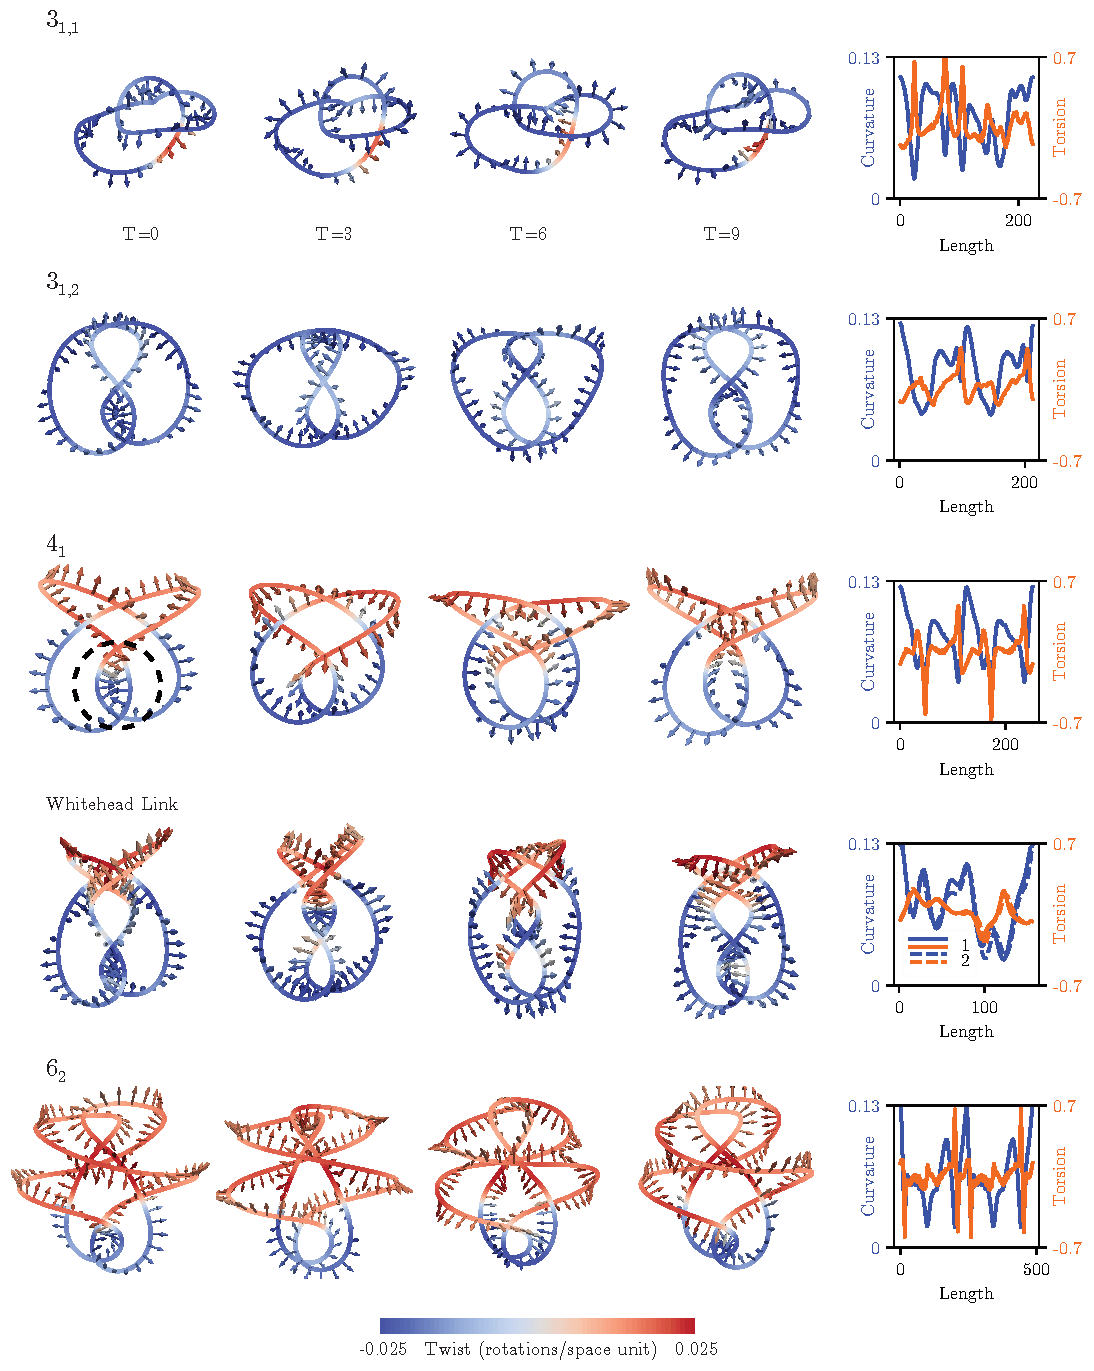
\includegraphics[width=0.95\textwidth]{\FitzHughNagumoFigures/StableKnots/StableKnotsFigure.pdf}
    \caption[Characterisation of stable knots.]{Geometries, vortex framings and twist distributions of our stable knots. Vector fields along curves indicate vortex framings, and are shown at four successive times across a (approximate) vortex rotation period. Curvatures and torsions shown correspond to the $T=0$ panels (there is slight intra-period variation) with the zero of arclength fixed to maximal curvature values. With the exception of the $4_1$ knot for which there is no distinction, all knots shown are the `right handed' chiral variant --- they rotate in a right handed sense about their direction of motion (down the page). Dotted circle highlights a half turn of a helix in the figure eight geometry, which may be extended to several half turns to give the initialisation geometries for the stable Whitehead link and $6_2$ knot shown. }
\label{fig:StableKnots}
\end{figure}

Figure~\ref{fig:StableKnots} shows the geometries, curvature and torsions as a function of arclength, vortex framings and twist distributions of the stable $3_{1,1}$, $3_{1,2}$ and figure eight knots. The evolution of their vortex framings at four successive intervals over a (approximate) vortex rotation period are indicated by the vector fields along the curves. Curvatures and torsions shown correspond to the geometries in the far left, $T=0$ panels (as discussed in \S \ref{subsec:DefiningTracking} there is slight intra-period oscillation), with the arbitrary zero of arclength fixed to coincide with maximal curvature values. We first note the striking twofold symmetry of both the $3_{1,2}$ and the $4_1$ knots; this symmetry is not a remnant of initial conditions, but emerges from the underlying dynamics. By contrast, the $3_{1,1}$ lacks any threefold symmetry. This is especially notable given that this state was reached starting from an exactly threefold symmetric torus knot geometry in \S \ref{sec:UnstableKnots}. It appears that the boundary stabilised trefoil reported in~\citep{Maucher2017} also lacks threefold symmetry, although it is unclear why this loss of symmetry does not occur for boundary stabilised torus knots of higher crossing number. A second striking feature of these stable knots is the tight synchronisation of the evolution of their framings. The framings of closely separated segments of the filament mesh~\citep{Henze1993}, the wavetip emanating from one segment being consistently met by a wavetip emanating from a spatially neighbouring segment, resulting in travelling waves of tightly synchronised wave activity running the length of the knot in a periodic fashion. The pattern is evident in the $3_{1,2}$ and figure eight knots, but is also present in the $3_{1,1}$, most clearly when one focuses on one of its three relatively straight segments; the framing of the curved lobes is twisted such that it meets the rotation of the wavetip emanating from the straight segment. Again, this meshing is an emergent property of the stable knot. 
\begin{figure}[htbp]
\centering
    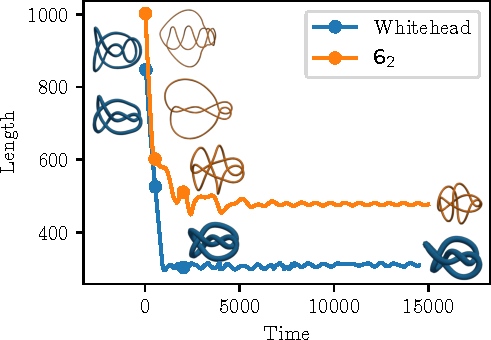
\includegraphics[width=0.65\linewidth]{\FitzHughNagumoFigures/Stable_Whitehead_6_2/Whitehead_6_2.pdf}
    \caption[Length evolution of novel stable knots.]{Length evolution of the Whitehead link and the $6_2$ knot with initialisation geometries made by extending the structure of the stable $4_1$ knot. Insets correspond to marked times.}
\label{fig:Whitehead_6_2}
\end{figure}

The similarity of the geometries and vortex framings of the $3_{1,2}$ and figure eight is suggestive of a recurrent structural motif. To investigate further we take the geometry of the the stable figure eight and use it as a starting point to construct new trial initialisation geometries. We do so in the simplest way possible --- as highlighted in the dotted circle around a section of the $T=0$ figure eight in figure \ref{fig:StableKnots}, the knot geometry contains a half-turn of a helix, which we may extend to an integer number of half-turns. Doing so gives a family of trial initialisation curves alternating between knots and two component links, the next two being the Whitehead link and the $6_2$ knot. Simulation reveals that such initialisation geometries evolve to apparently stable states. Figure \ref{fig:StableKnots} shows their detailed geometry, and in figure \ref{fig:Whitehead_6_2} we confirm their bulk stability up to $T=15000$. Both states share the twofold symmetry and tight synchronisation over a vortex rotation period found in the $3_{1,2}$ and figure eight knots, with especially close similarity in the geometry and twist distributions of the $4_1$, Whitehead link and $6_2$ knots. This similarity suggests that they arise as the start of a family of such stable knots which does not cleave along some existing sub-category of knots (for example torus knots) but rather arises specifically from the FitzHugh-Nagumo dynamics. As another demonstration of the importance of initial conditions, and a reminder that such states may have small basins of attraction, we note that the $6_2$ of \S \ref{sec:UnstableKnots} does not find this stable state over the times simulated.

In figure \ref{fig:KnotDynamics} we explore the dynamical properties of all stable knots found thus far. With the exception of the $3_{1,1}$, we find that each drifts along its axis of symmetry and rotates as a rigid body, with speeds and rotation rates summarised in figure \ref{fig:KnotDynamics}(a); these rates are computed by averaging the motion of the rigid body frame of the stable knot over $\Delta T = 2000$. An example of this motion is shown for the $6_2$ knot in figure \ref{fig:KnotDynamics}(b) (as can be seen in figure \ref{fig:Whitehead_6_2}, the Whitehead link and the $6_2$ knot have some long timescale periodic length modulation which corresponds to a slight oscillation in their velocity). The $3_{1,1}$ instead drifts in a helix as shown in figure~\ref{fig:KnotDynamics}(c), rotating about the helical axis as a rigid body, a reflection of its lack of threefold symmetry (a numerical fit to this helix~\citep{Enkhbayar2008} finds that it has radius $3.23$ and pitch $39.34$). The scale, and structure with knot size, of the drift velocities resembles that found for torus links in~\citep{Maucher2019}: within the family of knots discussed above, we see drift velocity decreasing with knot size. However, the complex geometries of the stable knots discussed here renders the explanation for this decrease given for torus knots (decreasing asymmetry between inner and outer parts of the torus as size increases) inapplicable. A reflection of this complexity is that, beyond consistency of scale, there is no clear accompanying pattern in the rotation rate data.

We briefly note that in the above discussion of vortex rotation sense, drift velocity and overall knot rotation sense we have not been careful to distinguish the possibly different behaviours of oriented or chiral variants from one another. All stable knots and links discussed above are isotopic to themselves under reversal of the orientation of any link component, however with the exception of the $4_1$ they are all chiral, and this chirality determines the rotation sense of the knot. In figures \ref{fig:StableKnots} and \ref{fig:KnotDynamics} we present variants rotating in a right handed sense about their drift velocity; left handed variants, with reversed twist distributions, also exist.

As discussed in \S \ref{sec:UnstableKnots},~\citep{Maucher2018} reports an increase in the rotation period of a stable unknot by $14\%$. We investigate whether similar shifts exist for other stable knots by looking at the spectra of their high frequency length oscillations. Figure~\ref{fig:KnotDynamics}(d) shows the spectra of all stable knots as measured over $\Delta T = 4000$ after they reach their stable configurations, alongside the spectra of the first $T=1000$ of the unknot and $4_1$ data shown in figure~\ref{fig:UnstableKnotsLength}. We include this second set of data for calibration and methodology validation, as during this time we expect the data to give the spectrum of a noninteracting knot, which should approximately correspond to $f_0$. As expected, the length oscillations of the noninteracting data are consistent with the fundamental vortex rotation frequency of $f_0=0.0898$, and do not vary with knot topology --- before inter-vortex interactions occur the global structure of the filament does not dramatically affect vortex rotation period. In fact, as this data is taken during the contraction of both knots, the observation that it shows purely spectral broadening suggests a negligible role for curvature in possible shifts to rotation frequency. As with the noninteracting data, the stable knot spectra show single peaks, but their frequencies are shifted relative to the noninteracting case on a scale which exceeds our estimate of curvature induced corrections. For all nontrivial knots, this shift is to a higher frequency (lower period), and its size is approximately constant; we obtain a period of $T=0.97T_0$. By contrast, the unknot alone shows a substantial shift to lower frequencies (higher period); we find an unknot rotation period of $T=1.19T_0$, consistent with the results of~\citep{Maucher2018}. That the situation for nontrivial knots is a shift to lower period relative to an isolated filament is intriguing, and suggests itself as a potential origin of the motion of the collision interface leading to the wave slapping observed in \S \ref{sec:UnstableKnots}. One important complicating factor in this sort of analysis is Doppler shift. Although the period of the stable unknot is higher than $T_0$, its velocity is $0.3$, a substantial fraction of the wavespeed $(1.9)$ in the medium. Using the data presented here this gives a Doppler shifted period for a stationary observer ahead of the unknot of only $1\%$ greater than $T_0$; in other words, at least for the unknot, relative filament motion is extremely important in determining the stability of a situation. A similar calculation for an observer behind the $4_1$ gives a Doppler shifted period of $T=0.975T_0$, a far less substantial shift. We speculate that these two facts, firstly that stable structures generically appear to have periods shifted below $T_0$, and secondly that even when the shift is to a higher period in the case of the unknot (extrapolating unknot behaviour to that of generic anti-parallel strands) this increase is compensated for in a directional manner by Doppler shift, give an intrinsically unstable dynamics in which the formation of any interacting structure hinders further formation via wave slapping.

\begin{figure}[htbp]
    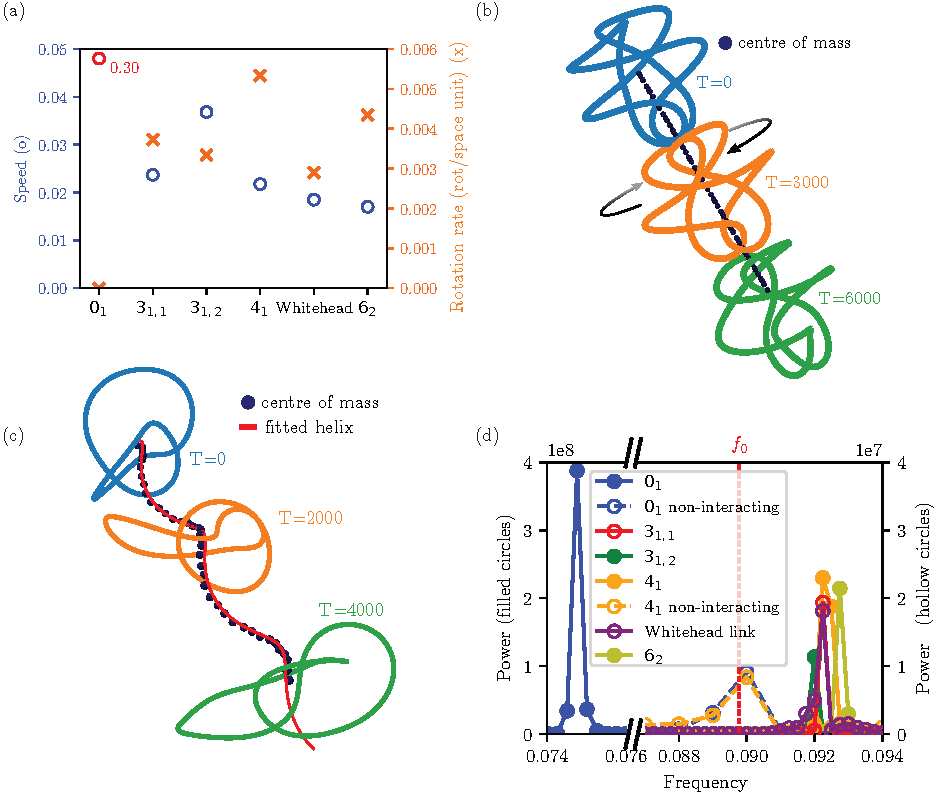
\includegraphics[width=0.99\textwidth]{\FitzHughNagumoFigures/KnotDynamics/KnotDynamicsFigure.pdf}
    \caption[Dynamics of stable knots.]{Dynamics of stable knots. (a) A summary of drift speeds and rotation rates for all known stable knots. Note that the velocity given for the $3_{1,1}$ is that along its helical axis. (b) Drift and rotation of the $6_2$ knot. Shown are centres of mass taken at $T=100$ intervals (blue dots), and snapshots of the geometry at $T=3000$ intervals; between each snapshot the knot has rotated $\sim 20$ times. (c) The $3_{1,1}$ drifts along a helical path (fitted red curve), rotating about the helix axis as a rigid body. (d) Power spectra of high frequency oscillations in knot length data. Before inter-vortex interactions occur, the oscillation period is the same as ${f_0}$. All non-trivial stable knots show a similar shift to higher vortex rotation frequencies ($T=0.97T_0$), with the unknot alone showing a shift to lower frequencies ($T=1.19T_0$).}
\label{fig:KnotDynamics}
\end{figure}
\section{\label{sec:Discussion}Discussion}

We have presented a survey of the bulk dynamics of knotted vortices in the FitzHugh-Nagumo model covering prime knots up to crossing number $N=8$. Although the simplest knots --- the unknot, trefoil and figure eight --- possess stable states and exhibit a fascinating dynamics of untangling without reconnections, this is not repeated for any of the other knots in our survey. The general trend is an irregular dynamics, marked by sustained periods of length expansion of parts of the knot, the cause of which we have directly shown to be a long-range wave slapping interaction. In several cases, this wave slapping led to strand reconnections and topology change, phenomena which appear to be associated more with the geometry of the wavefield than the topology of the vortex. 

For those stable knots found in our initial survey, we have tested the effectiveness of the FitzHugh-Nagumo flow in untangling a wide variety of initial conditions. Although the dynamics successfully untangled all but one initial geometry over the time simulated, we saw that in the case of the figure eight knot this untangling was far from monotonic, and that the same wave slapping dominating high crossing number knot behaviour may also cause low crossing number knots to substantially increase in length before untangling. These results stand in contrast to those of~\citep{Maucher2016} and our own on the rapid untangling of unknots. We gave a detailed characterisation of the geometry and dynamics of all known stable vortices in the bulk, including the tight synchronisation of their associated wavefields, their motion through the medium and natural rotation periods, and shifts in the spectra of their high frequency length oscillations. In addition to the already known trefoil and figure eight knots, we found stable forms for the Whitehead link and $6_2$ knot, both of which appear to come from the same `family' of knots as the figure eight. While in the former case, the basin of attraction appears to be large, the same cannot be said for the latter, at least for the timescales of the simulations we have run. 

Throughout this chapter, we have emphasised the importance of the collision interface on understanding long timescale vortex dynamics. Although we have seen many examples of its importance, an understanding of its own dynamics is currently qualitative at best. As a first step towards rectifying this, it would be interesting to directly study the evolution of local rotation rate along a vortex to fully disentangle the possible effects of curvature, twist and interactions. Turning from general dynamical questions to the details of stable states, beyond noting close similarities between those found we have not proposed principles by which their geometry and behaviour may be understood. A detailed description appears challenging, but the observed wavefield synchronisation, and similarities in the size of spectral shifts, of \S\ref{sec:StableKnots} offers a global organising principle from which one might try to predict geometries. When discussing stability we have contrasted our own results in the bulk with those on torus knots and links that have been found near no-flux boundaries~\citep{Maucher2017,Maucher2019}, detailing where results overlap (the stability of the trefoil and figure eight) and where they diverge. Although we have seen that boundary stabilisation is more complex than simply a suppression of the sproing instability, its exact nature remains unclear, and deserves further study. 

The features of the FitzHugh-Nagumo model at the parameter values studied here which are conducive to the formation of stable knots --- short-range inter-vortex repulsion, a contractile filament law of motion --- are offset by other undesirable features, primarily wave slapping. Parameter choices were originally made in~\citep{Henze1993} on the basis that such values gave two-dimensional vortices with desirable properties and three-dimensional simulations were computationally feasible. It would be interesting to revisit these choices armed with new criteria for a desirable set of parameters. For example, we might search for parameters (or indeed models) such that rotation frequency is seen to decrease with twist and interactions. A related question is to explore whether wave slapping interactions have any role in enhancing untangling as well as hindering it --- in other words, whether the untangling aspect of the dynamics can be captured in a local geometric model. Here the tubed knot of \S\ref{sec:UnstableKnots} offers some hints; in preliminary simulations of tubed versions of the tangled unknots of \S\ref{sec:StableKnots} we do not see substantial differences in the untangling times between tubed and untubed unknots. It may be the case that, although the full dynamics appear extremely difficult to capture with a local geometric model, such a model offers insight for the restricted case of unknot untangling. This is especially interesting given the apparent contrast between the untangling dynamics seen here and those utilised by line tension minimisation methods~\citep{Maucher2016}. 

Stable vortex rings have been realised experimentally and successfully described using existing theory~\citep{Steinbock2006, Azhand2014, Totz2015}. As such, although one expects the precise details of knot stability to be specific to the system studied, we believe that our exploration of the phenomena seen here --- the importance of wave slapping, bulk simplification of low crossing number knots, frequency shifts in stable knots --- is of direct experimental interest for a general excitable medium, outside of the details of the FitzHugh-Nagumo model. 

 \chapter{Bend Geometry in Liquid Crystals}
\label{ch:TwistBend}
\section{Introduction}
Geometric structures pervade the physics of liquid crystals. Famously, it was the geometry of focal conics that led Friedel to an understanding of smectics~\citep{friedel1910}. This has been followed by geometric models of developable domains~\citep{kleman80,bouligand80}, screw dislocations and grain boundaries~\citep{kamien99}, columnar phases on curved substrates~\citep{santangelo07}, and the beautiful explanation of the frustration in blue phases \citep{sethna83}. The geometry of vector or nematic-like order was introduced in \S\ref{subsec:Geometry} where we gave Frank's elasticity of nematics \eqref{eq:FrankFreeEnergy}, in which the fundamental modes of distortion --- splay, twist, bend, biaxial splay --- are named for their geometric character. Corresponding to the symmetries of this elasticity we had the decomposition \eqref{eq:GradientDecompositionpar}, \eqref{eq:GradientDecompositionperp} of director gradients into components parallel ($\nabla^L \w n$) and perpendicular ($\nabla^\xi \w n$) to $\w n$. Focusing on the shape operator $\nabla^\xi \w n$, we saw that there were geometric singularities called umbilic lines \citep{Machon2016b}, zeros of the deviatoric part of $\nabla^\xi \w n$, $\Delta$, which describes directions of principal curvature. The importance of umbilic lines is brought to the fore when they have direct energetic consequences, as in a cholesteric liquid crystal, minimally described by 
\begin{equation}
    F_{\mathrm{ch}} = \frac{K}{2}  \int d^3 {\bf r}\left(|\nabla {\bf n}|^2 +2 q_0 {\bf n} \cdot \nabla \times {\bf n} \right),
    \label{eq:CholestericFreeEnergy}
\end{equation}
a modification of \eqref{eq:FrankFreeEnergy} in which all elastic constants are set to the same value $K$ and the twist energy is shifted to have a minimum at $\w n \cdot \nabla \times \w n = -q_0$ \citep{deGennes1992}. The groundstate is given by any director field equivalent to $\w n = (\cos q_0 z, \sin q_0 z, 0)$ (with nonzero twist $q_0$), where the local $z$ direction is set by the pitch axis, $\w p$, a second vector distinct from the line field $\w n$ which gives the local axis of twisting in the cholesteric. The eigenvectors of $\Delta$ determine $\w p$ \citep{Bellar2014, Machon2016b}, and umbilics in cholesterics then correspond to energetically costly defects in the pitch axis called $\lambda$ lines \citep{Bellar2014}. Cholesterics themselves support an increased variety of metastable states relative to the nematic phase, with many topological configurations including Skyrmions, Hopfions and other knotted solitons (some of which are shown and discussed in \S \ref{subsec:SkyrmionsAndHopfions}), novel textures of shells and droplets, and constellations of point defects~\citep{posnjak17}. Within these solitons, $\lambda$ lines might be considered `fingerprints', naturally localised geometric structures describing energetic frustration, which also convey global topological information about the texture as zeros of a section of the nontrivial part of $\xi^* \otimes \xi$ directly derived from $\w n$. 

This chapter is about the geometry and topology in the part of $\nabla \w n$ not examined above, $\nabla^L \w n= \w n^* \otimes \nabla_\w n \w n$, determined by the bend vector $\w b:= \nabla_\w n \w n$. By analogy with the description of the shape operator, umbilic lines and cholesterics given above, several questions suggest themselves: If the geometry of $\Delta$ is the geometry of surface curvatures, what is the geometry of $\w b$? Do cousins of umbilic lines exist, and if so what is their structure and topological significance? What types of `bend solitons' might we expect? And, if cholesterics are the natural setting to study umbilics, what is the natural setting to study bend? The recently discovered twist-bend nematic~\citep{Cestari2011, Chen2013, Borshch2013, Lavrentovich2018} is one answer to this last question, providing a system in which the geometry of bend is naturally brought to prominence. In these systems the molecules have a bent-core architecture that leads to an energetic preference for non-zero bend. The observed phase, and apparent theoretical groundstate, has a heliconical ordering that is intermediate between ordinary nematics and cholesterics. As such, we might expect analogous textures and topological states to those observed in cholesterics. One key difference between the systems, however, is that the cholesteric energy \eqref{eq:CholestericFreeEnergy} is intrinsically chiral --- left handed and right handed twist have different energies. By contrast, the twist-bend nematic energy is achiral, the ground state spontaneously picking one of two equal energy heliconic (hence chiral) states. A second difference is that the bend is identically zero in the cholesteric ground state.

In \S\ref{sec:Elements} we will describe the fundamental geometry and topology of bend, relating it to the curvatures and torsions of families of integral curves, and show that cousins of umbilic (or $\lambda$) lines exist, which we call $\beta$ lines. Their structure, including a natural notion of self-linking, will be discussed in \S\ref{sec:BendStructure}. These $\beta$ lines, zeros of a section of $\xi$, provide topological information analogous to umbilics; they give a Skyrmion count, and are capable of distinguishing textures of different Hopf invariant. We explore their topological significance in \S\ref{sec:TopologicalSignificance}. Throughout, we will use the twist-bend nematic as a model system, providing simulation results of twist-bend Skyrmions and Hopfions. As such, we give a standalone introduction to twist-bend nematics in \S\ref{sec:TwistBendNematics}. We conclude with a discussion of avenues for further work in \S\ref{sec:Discussion}. 

\section{Elements of the global geometry and topology of bend} 
\label{sec:Elements} 
We firstly specify a few technical details brushed over in \S \ref{subsec:Geometry}. Vector bundles over a contractible space (like $\mathbb{R}^3$) are trivial \citep{MilnorStasheffBook}, as are homotopy classes of maps from this space into any other (in our case specifically $S^2$ or $\mathbb{R}P^2$)~\citep{Hatcher2012}. So in order to see topologically interesting features, such as a nontrivial Euler class for $\xi$, our material must be topologically nontrivial. We will denote it by a general 3-manifold $M$, and typically have in mind experimentally accessible examples like $S^3, D^2 \times S^1$, $S^2 \times S^1$, perhaps also $T^2 \times S^1$ or $T^3$, as well as the plethora of 3-manifolds given by knot complements\footnote{Not all of these examples actually can support nontrivial $\xi$! For example, $H^2(S^3)=0$.}. $M$ has a metric, which we denote $\langle \bullet , \bullet \rangle$ or, when using vectors and there is no chance of ambiguity, with the dot product notation $\bullet \cdot \bullet$. The manifold is considered equipped with its standard metric compatible connection $\nabla$. We will also freely use vectorial and vector calculus notions such as cross products, gradients and curls, for example writing $(\w n \cdot \nabla \w) \w n = \nabla_{\w n} \w n$, where on the left hand side with have the vector calculus gradient and dot product, and on the right the connection. These vectorial concepts may be defined on a general 3-manifold in terms of differential forms, wedge products and so forth \citep{Lee1996, Frankel2015}, however typically we think of our 3-manifold as a subset of $\mathbb{R}^3$ with some nontrivial boundary conditions which allow us to compactify the space (for example imposing fixed far field boundary conditions on $\mathbb{R}^3$ allows compactification to $S^3$). As such, we may locally consider the manifold $\mathbb{R}^3$ with its standard connection and metric, and think of vectorial notions in the familiar direct way, moving freely between them and the alternative presentation involving connections and differential forms. 

The bend is the change of the director field along itself, ${\bf b} = \nabla_{{\bf n}}{\bf n}=-{\bf n}\times\nabla\times{\bf n}$, and is a globally defined vector whose sign does not reverse under the replacement of ${\bf n}$ by $-{\bf n}$. As such, it is well defined for a line field, however in this chapter we will restrict our attention to orientable textures (those without disclination lines) in which $\w n$ can be considered a unit vector. As ${\bf n}$ is a unit vector, the bend is everywhere orthogonal to it, ${\bf b}\cdot{\bf n}=0$ --- that is, $\w b$ is a section of $\xi$. Setting ${\bf b}_\perp:={\bf n}\times{\w b}$ and denoting their normalised vectors ${\bf e}_1 := \w b/|\w b|$, $\w e_2 := \w b_\perp/|\w b_\perp| = \w n \times \w e_1$ we have a local orthonormal frame $({\bf e}_1, {\bf e}_2, {\bf n})$. Considering a single integral curve of the director, this frame is exactly the Frenet-Serret frame $({\bf e}_1, {\bf e}_2,{\bf n}) = (\w N, \w B, \w T)$ \citep{DoCarmoBook}, where $\w T, \w N, \w B$ are the tangent, normal and binormal to the integral curve, and in terms of curve geometry $\w b = \kappa \w N$, where $\kappa$ is the classical curvature. Continuing in the same vein, the torsion of the integral curves is given by $\tau  = \langle \w e_2 , \nabla_\w n \w e_1 \rangle $, a measure of how the Frenet-Serret frame spins about the tangent as one moves along the curve. For any curve, its torsion $\tau$ may be interpreted as the connection one form corresponding to the restriction of the ambient connection onto the curve's normal bundle. For the family of integral curves given by the director we interpret it as one component of a connection one-form on the bundle $\xi$,  
\begin{equation}
    A := \langle \nabla \w e_1 ,\w e_2 \rangle = \frac{\langle \nabla \w b ,\w b_\perp \rangle}{\langle \w b,\w b \rangle}. 
    \label{eq:1form}
\end{equation}
This 1-form and its associated curvature $\Omega = dA$ will enter in a fundamental way into the characterisation of the director field, orienting bend zeros and giving a count of Skyrmions. A few remarks about \eqref{eq:1form} are in order. Firstly, the connection $\nabla$ here is a connection on the bundle $\xi$, and is globally well defined as the restriction of the ambient connection on the manifold to the plane field $\xi$. Equivalently, it is the pullback connection induced by the map ${\bf n}: M \rightarrow S^2$ \citep{Lee1996}.\footnote{$\w n$ is a unit magnitude section of $TM$. However, 3-manifolds are parallelisable \citep{Geiges2009}, meaning an everywhere nonzero basis can be chosen for the entire bundle. Relative to such a basis $\w n: M \rightarrow S^2$.}. The sections $(\w e_1,\w e_2)$ are, however, only well defined on the complement of the bend zeros (which we come to in a moment), and this carries through to the 1-form $A$. 

The bend is a vector in three-dimensional space, and a generic such vector vanishes at isolated points. However, the constraint that it be orthogonal to the director makes it atypical, having only two degrees of freedom --- $\w b$ is locally a map $\mathbb{R}^3 \rightarrow \mathbb{R}^2$. As a result, the set of points where it vanishes is one-dimensional and forms a set of fundamental curves in the material that are characteristic of the director field. On these lines $\w b = \kappa \w N = 0$, so they correspond to points of inflection in the integral curves of ${\bf n}$, where the curvature $\kappa$ vanishes. We might think of these zeros as `inflectional lines', but we shall refer to them as $\beta$ lines by informal analogy with $\lambda$ lines. Finally, as discussed in \S\ref{subsec:Geometry}, the zeros of any section of an (orientable) vector bundle encode its Euler class. More precisely, the $\beta$ lines, counted with appropriate sign, are Poincar\'e dual to the Euler class of $\xi$, $e(\xi) \in H^2(M)$ \citep{BottTuBook,Hatcher2012, Geiges2009}. This is certainly true, however the $\beta$ lines are more than this --- they are not just any section, freely chosen within $\xi$. Rather, they are directly derived from the director $\w n$, and cannot be varied independently of it. One thus expects them to encode more information than an arbitrary section of $\xi$; we shall return to this point in \S\ref{sec:Discussion}. 
\section{Twist-bend nematics} 
\label{sec:TwistBendNematics}
The twist-bend nematic, $N_{\mathrm{tb}}$, is a recently discovered phase of liquid crystal in which the director adopts a spontaneous nonzero magnitude of bend \citep{Lavrentovich2018}. Originally suggested by Meyer \citep{Meyer1976}, the idea was not actively pursued until an article of Dozov's \citep{Dozov2001} in which he considered the possibility of the bend elastic constant, $K_3$ in \eqref{eq:FrankFreeEnergy}, becoming negative, with the free energy then stabilised from below by higher order derivatives. Everywhere constant magnitude bend is not possible in two dimensions \citep{Niv2018}, however provided one accepts an accompanying twist or splay deformation, it is possible in three dimensions. Of these possibilities Dozov focused on the twist-bend case, predicting a heliconical director shown in figure \ref{fig:Bananas}(a)
\begin{equation}
\w n = (\sin \theta \cos q z, \sin \theta \sin q z , \cos \theta),
\label{eq:TwistBendDirector}
\end{equation}
where $2\pi/q$ is the heliconical pitch and $\theta$ is the tilt angle. The bend vector in this heliconical state is $\w b = q\sin \theta \cos\theta (-\sin q z, \cos q z, 0)$ and the twist is $- q \sin^2 \theta$. As $\theta \rightarrow 0$ we recover a simple nematic, and as $\theta \rightarrow \pi/2$ we obtain the cholesteric ground state. A more recent theoretical approach, closer in spirit to Meyer's original work, is to keep $K_3$ positive but augment the director $\w n$ with a vector order parameter $\w p$, the shape polarisation, shown in figures \ref{fig:Bananas}(a),(c) \citep{Shamid2013}. $\w n$ and $\w p$ together describe a banana shaped (`bent-core') molecule, with $\w n$ specifying the long axis of the banana (which respects $\w n \rightarrow -\w n$) and the direction and magnitude of $\w p$ specifying the orientation and bendiness of the banana in the plane perpendicular to $\w n$. Spontaneous bend may be generated through a coupling to polarisation via a term in the free energy like $-\w p \cdot (\w n \cdot \nabla) \w n=- \w p \cdot \w b$, expressing the steric preference of banana shaped molecules to pack into configurations with nonzero director bend. A minimal free energy, following \citep{Shamid2013}, is
\begin{figure}[htbp]
    \centering
    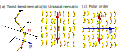
\includegraphics{\TwistBendFigures/Bananas.pdf}
    \caption[Twist-bend nematics.]{(a) The heliconical ground state of a twist-bend nematic, with director $\w n$ and shape polarisation $\w p$ of the banana shaped molecules shown. $\w p$ is parallel to the bend vector $\w b$ of the director. (b,c) Just as a uniaxial liquid crystal can exist in either an isotropic or nematic phase despite the individual molecules being rod-like, a banana shaped molecule does not automatically imply the twist-bend state --- these polar molecules may have their orientations randomly aligned to give no net shape polarisation, creating a uniaxial nematic phase. Figures reproduced from \citep{Lavrentovich2018}.}
    \label{fig:Bananas}
\end{figure}
\begin{equation}
    F_{\mathrm{tb}} =  \int d^3 {\bf r}\ \frac{K}{2}|\nabla {\bf n}|^2 +\frac{C}{2}|\nabla {\bf p}|^2 -\lambda \w p \cdot (\w n \cdot \nabla)\w n + \frac{u}{4}(1 - |\w p|^2)^2
    \label{eq:TwistBendFreeEnergy}
\end{equation}
where $K$ is a single Frank elastic constant for the director, $C$ is the same for the polarisation, $\lambda$ sets the strength of coupling between bend and polarisation, and $u$ sets the scale of the bulk ordering energy. One may coarse grain $\w p$ out of this free energy, reproducing Dozov's theory with an effective bend constant $K_3^{\mathrm{eff}} = K_3 - (2\lambda^2/u)$, which becomes negative if the ratio $\lambda^2/u$ is large enough \citep{Meyer2016}. The ground state of \eqref{eq:TwistBendFreeEnergy} appears to be given by \eqref{eq:TwistBendDirector}. Sending $u \rightarrow \infty$ in \eqref{eq:TwistBendFreeEnergy}, as is the case deep in the twist-bend phase, $|\w p|=1$ and $\w p$ is assumed to have the form  
\begin{equation}
\w p = (- \sin q z, \cos q z ,0).
\label{eq:TwistBendPolarisation}
\end{equation}
This limit is useful for theoretical intuition, although in all simulations of the free energy \eqref{eq:TwistBendFreeEnergy} presented in this chapter we allow the magnitude of $\w p$ to vary. Substituting the forms \eqref{eq:TwistBendDirector}, \eqref{eq:TwistBendPolarisation} into \eqref{eq:TwistBendFreeEnergy} one may determine the heliconical parameters in terms of those in the free energy,
\begin{align}
    \label{eq:theta}
    \cos 2 \theta &= \left( 1+ \frac{2C}{K} \right) - \left( \frac{4C}{K}  \left( 1+ \frac{C}{K} \right) \right)^\frac{1}{2},\\
    \label{eq:q}
    q &= \frac{2 \lambda}{K} \cot 2 \theta,
\end{align}
which may also be written
\begin{align}
    \frac{\lambda}{K} = \frac{q \tan 2 \theta}{2}, \quad 
    \frac{C}{K} = \frac{\sin^4\theta}{\cos 2 \theta}.
\end{align}
In terms of dimensionless variables $\lambda/K , C/K$ the magnitude of the heliconical bend is
\begin{align}
    |\w b| = q\sin\theta\cos\theta = \frac{\lambda}{K}\left( \left( 1+ \frac{2C}{K} \right) - \left( \frac{4C}{K}  \left( 1+ \frac{C}{K} \right) \right)^\frac{1}{2}\right).
    \label{eq:magb}
\end{align}
\begin{figure}[htbp]
    \centering
    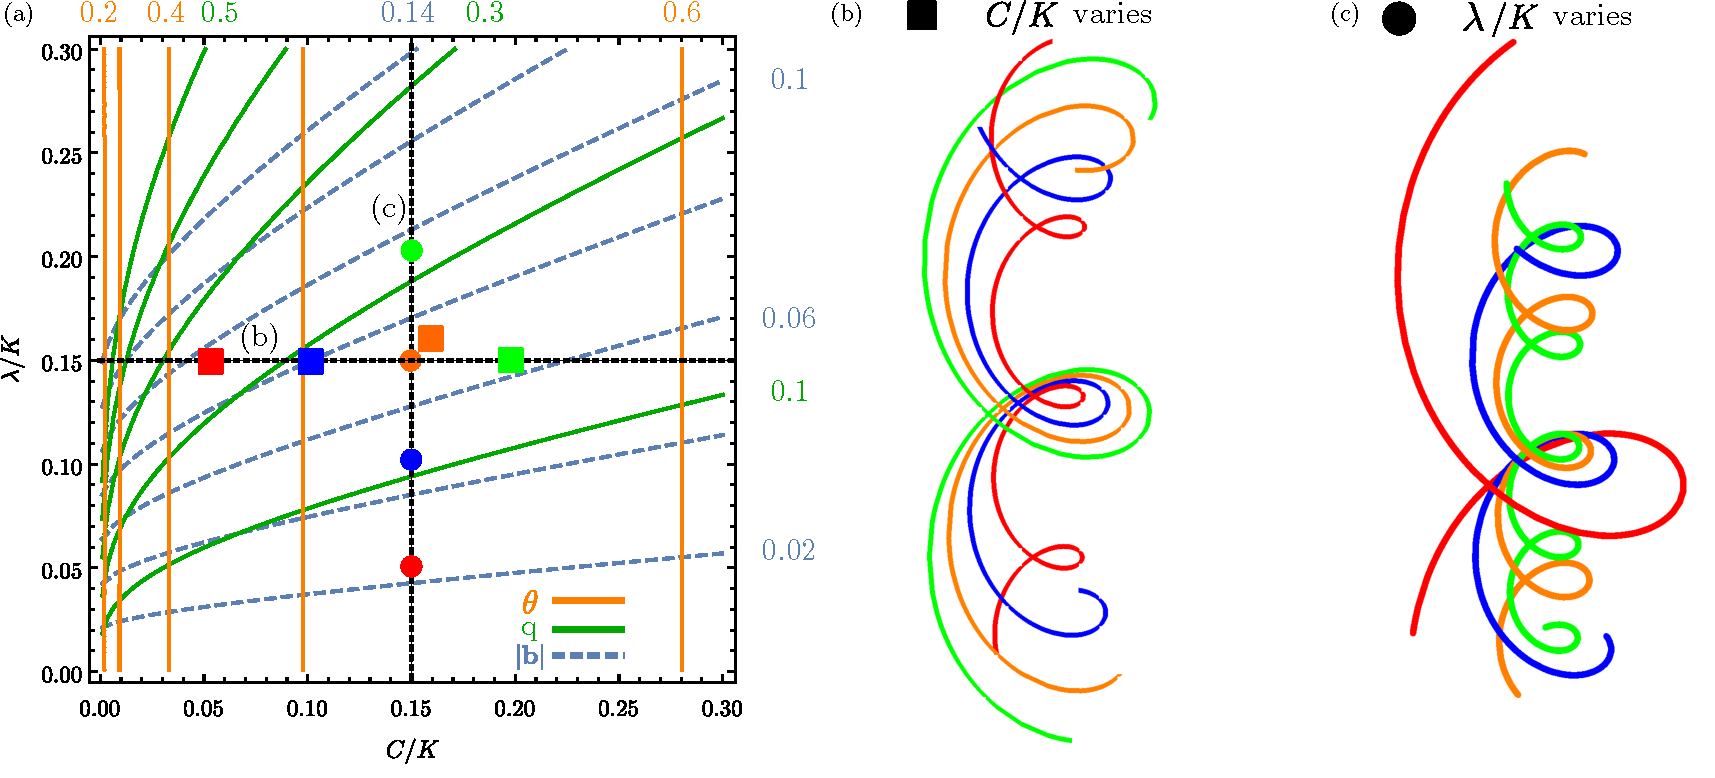
\includegraphics[width=\textwidth]{\TwistBendFigures/HeliconicalGroundState.pdf}
    \caption[Heliconical ground state of a twist-bend nematic.]{(a) Contour plots of $\theta$ \eqref{eq:theta}, $q$ \eqref{eq:q} and $|b|$ \eqref{eq:magb} against $C/K, \lambda/K$ for the heliconical ground state \eqref{eq:TwistBendDirector} of the free energy \eqref{eq:TwistBendFreeEnergy}. Coloured squares and circles are particular values of $(C/K, \lambda /K)$ for which the corresponding integral curves of the director are shown in (b),(c).}
    \label{fig:HeliconicalGroundState}
\end{figure}
In figure \ref{fig:HeliconicalGroundState}(a) we plot $\theta, q, |\w b|$ as functions of $C/K, \lambda/K$. Fixing $\lambda/K$ and increasing $C/K$ causes the cone angle to increase towards an asymptotic value of $\pi/4$, and both wavevector and bend magnitude to decrease. Fixing $C/K$ and increasing $\lambda/K$ causes wavevector and bend magnitude to increase, with the cone angle unchanged. The integral curves of the director \eqref{eq:TwistBendDirector} are given by the helices
\begin{align}
    (x(t),y(t),z(t)) = (\frac{1}{q} \tan \theta \sin qt, \frac{1}{q} \tan \theta \cos qt,t),
\end{align}
and in figures \ref{fig:HeliconicalGroundState}(b),(c) we show the effects of varying $C/K, \lambda/K$ on these integral curves.

Theoretical prediction of the twist-bend nematic predated its experimental observation by decades \citep{Lavrentovich2018}, with optical microscopy experiments in the period $1993$--$2013$ suggesting the existence of a low temperature `$N_\mathrm{x}$' state in a variety of flexible dimers, which supported focal conics as well as other hallmarks of a layered structure, but without an accompanying density wave (as in a smectic) and a periodicity too small to resolve (in contrast to a cholesteric). More direct observations came from freeze-fracture transmission electron microscopy in 2013 \citep{Borshch2013}, with an $N_{\mathrm{tb}}$ phase directly observed in cyanobiphenyl-$(\mathrm{CH}_2)_7$-cyanobiphenyl (CB$7$BC) with an extremely small pitch of $8$-$9$nm. Currently there are over $100$ compounds known to exhibit this phase, with prevailing pitch lengths on the nanometre scale \citep{Lavrentovich2018}. In comparison to cholesterics, with pitches in the $\mu$m, this certainly represents a current experimental difficulty in generating topologically nontrivial textures in these systems, with typical techniques --- optical visualisation and manipulation using fabricated colloids \citep{Tasinkevych2014} or lazer tweezers \citep{Tkalec2011,Copar2015,Ackerman2017} --- inapplicable at such scales. 
\label{sec:GeometryTopologyOfBend}
\section{The structure of $\beta$ lines}
\label{sec:BendStructure}
Consider the 1-form $B := \langle b,b \rangle A$ and its dual vector $\w{B} := \langle B, \bullet \rangle$. The vector $\mathbf{j} := \nabla \times \mathbf{B}$ points along the $\beta$ lines, orienting them according to the circulation of $A$ as shown in figure~\ref{fig:BetaLines} \citep{Machon2016b}. To see this, consider a local trivialisation $(\w d_x, \w d_y,\w n)$ in a tubular neighbourhood around the $\beta$ line. Unlike $(\mathbf{b}, \mathbf{b}_\perp)$, $(\w d_x, \w d_y)$ are nonzero throughout the neighbourhood. In such a trivialisation, ${\bf b} = b_x \w{d}_x + b_y \w{d}_y,\ {\bf b}_\perp = b_x \w{d}_y - b_y \w{d}_x,\ \langle \w b, \w{b} \rangle = b_x^2 + b_y^2$. Expanding $A$ one finds
\begin{equation}
    A = \frac{b_x d b_y - b_y d b_x}{b_x^2 + b_y^2}+ \omega
    \label{eq:localA}
\end{equation}
where \omega := $\langle \w{d}_y, \nabla \w{d}_x \rangle$ is the connection $1$-form associated to $\nabla$ when using this local trivialisation. $(b_x,b_y,s)$, where $s$ is arclength along the $\beta$ line, form a local coordinate system with $z$-axis tangent to the $\beta$ line and given by $\nabla b_x \times \nabla b_y/|\nabla b_x \times \nabla b_y|$ --- generically $(b_x, b_y)$ vanish linearly, so $\nabla b_x, \nabla b_y$ are non-zero on the $\beta$ line and the coordinate system is well defined. We may also define the associated cylindrical polar system $(\rho,\theta,z)$\footnote{Remember, however, that the vectors $\nabla b_x/|\nabla b_x|$ and $\nabla b_y/|\nabla b_y|$ are not orthogonal and so there is a Jacobian between this and a `true' polar system.}, in which $A = d\theta + \omega$. The azimuthal 1-form $d\theta$ itself is undefined on the $\beta$ line, diverging relative to the smooth contribution $\omega$, and as such the essential behaviour of $A$ around the $\beta$ line is simply that of $d \theta$ (figure~\ref{fig:BetaLines}). Multiplying \eqref{eq:localA} through by $b_x^2 + b_y^2$, $\w{B} = b_x \nabla b_y - b_y \nabla b_x + (b_x^2 + b_y^2) \langle \omega, \bullet \rangle$  and on the $\beta$ line $\w{j} = \nabla \times \w{B} = 2 \nabla b_x \times \nabla b_y$. In terms of differential forms, on the $\beta$ line $dB = 2 d b_x \wedge d b_y$ and $\star dB$ is dual to $\w j$, where $\star$ denotes Hodge duality. We emphasise that $A$ and $d\theta$ are defined along the entire tubular neighbourhood of a generic $\beta$ line (with the line itself cut out), providing a canonical orientation.
\begin{figure}[htbp]
    \centering
    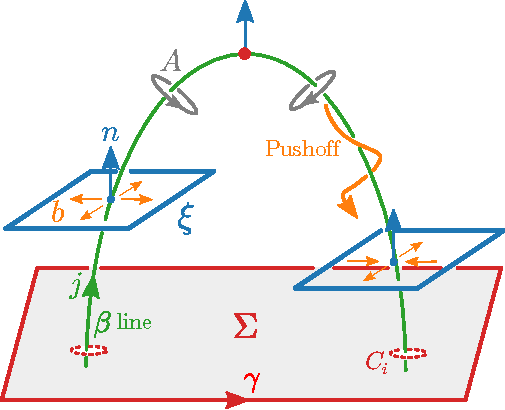
\includegraphics[keepaspectration, width=0.7\linewidth ]{\TwistBendFigures/BetaLine6.pdf}
    \caption[The structure of $\beta$ lines.]{The bend $\w n$ (orange arrows), a section of the bundle of planes $\xi$ (blue planes) which are perpendicular to the director $\w n$ (blue arrows), vanishes along curves called $\beta$ lines (green curve). The 1-form $A$ \eqref{eq:1form} (grey) circulates around these $\beta$ lines, providing a global orientation vector $\w j$. The figure shows a Legendrian point in the $\beta$ line (red dot), where $\w n \cdot \w j =0$, and across which the index of the $\beta$ line $I_\beta^\xi$, which characterises its local profile, changes.}
    \label{fig:BetaLines}
\end{figure}

\subsection{The local structure of $\beta$ lines}
\label{subsec:BendLocalStructure}
We may investigate the local structure of $\w b$ about a $\beta$ line via a Taylor series. Generically this series is governed by linear terms and so its structure is given by $\nabla \w b$ evaluated on the $\beta$ line. We have already seen that the director $\w n$ splits $T \mathbb{R}^3\approx L \oplus \xi$, with a corresponding splitting of $\nabla \w n$ into two pieces, $\nabla^L \w n $ and $\nabla^\xi \w n$, in \S\ref{subsec:Geometry}, and one way to proceed is to do same to $\nabla \w b$. However, the $\beta$ line itself, in combination with $\w n$ along it, provides us with more structure than a single splitting --- it gives a canonical way to further split $\xi$, giving an adapted framing with which several other planes and splittings may then be defined. In figure \ref{fig:Splittings}(a) we show the $\beta$ line and $\w n$ at a generic point, where $\w n$ and $\w j$ are neither parallel nor perpendicular. The normalised cross product $\w n \times \w j$ defines a vector $\w n_\lambda := \w n \times \w j/| \w n \times \w j|$ and orthogonal plane $\lambda$, and we define a third vector $\w n_\chi := \w n_\lambda \times \w n = (\w j - (\w n\cdot \w j)\w n)/|\w j - (\w n\cdot \w j)\w n|$, the normalised projection of $\w j$ onto $\xi$, with associated orthogonal plane $\chi$. Setting $(\w d_x, \w d_y, \w n) = (\w n_\chi, \w n_\lambda, \w n)$ gives an adapted frame for the $\beta$ line, with the line itself always in the $\lambda$ plane. Note immediately that by construction, $\w n_\chi \cdot \w j \geq 0$, and further that this frame is undefined if $\w n \parallel \w j$. Across such points both $\w n_\chi$ and $\w n_\lambda$ change sign discontinuously, and the framing undergoes a $\pi$ rotation (as unoriented planes $\chi$ and $\lambda$ may be extended by continuity) --- this situation is shown in figure  \ref{fig:Splittings}(b), and we shall return to it in a moment. As well as $\xi, \chi$ and $\lambda$, we also have the plane perpendicular to $\w j$ itself, given by $\mathrm{ker}(\star dB)$ and denoted $\alpha$. Loops in these planes measure winding about the $\beta$ line. We have two limiting cases, shown in figures \ref{fig:Splittings}(b) and (c). In figure~\ref{fig:Splittings}(b), $\w  n \parallel \w j$, $\xi = \alpha$ and a loop in $\chi$ intersects the $\beta$ line --- if we try to measure winding on this plane we encounter degenerate behaviour. In figure~\ref{fig:Splittings}(c) $\w n \perp \w j$, $\chi = \alpha$ and a loop in $\xi$  intersects the $\beta$ line, likewise showing degenerate behaviour. This latter case, where $\w n \cdot \w j= 0$, we refer to as a Legendrian point \citep{Geiges2009}. One notes that the degeneracy in figure \ref{fig:Splittings}(b) is of higher codimension than that in figure \ref{fig:Splittings}(c) --- in figure \ref{fig:Splittings}(c) we require one component of a unit vector to vanish, giving a codimension $1$ degeneracy, whereas in figure \ref{fig:Splittings} two must vanish, giving codimension $2$.
\begin{figure}[htbp]
    \centering
    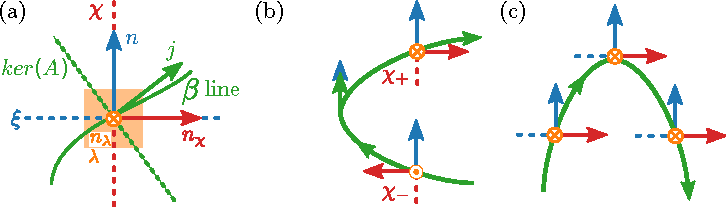
\includegraphics[keepaspectration, width=0.99\linewidth ]{\TwistBendFigures/Splittings.pdf}
    \caption[A canonical framing of $\beta$ lines.]{(a) At a generic point on a $\beta$ line we have a canonically defined triple $(\w n_\chi, \w n_\lambda, \w n)$ with orthogonal planes $(\chi,\lambda, \xi)$, as well as the tangent to the $\beta$ line $\w j$ and its orthogonal plane $\alpha$. This framing breaks down in the situation shown in panel (b), where  $\w n \parallel \w j$ and $\w n_\lambda$ is undefined, a codimension $2$ degeneracy. In (c) we show a Legendrian point where $\w n \cdot \w j = 0$, a codimension $1$ degeneracy. Measuring on a consistently oriented plane across these degeneracies (in other words using either $\chi_-$ or $\chi_+$ across the degeneracy in (b)), in (b) $I^\chi_\beta$ changes sign and in (c) $I^\xi_\beta$ changes sign.}
    \label{fig:Splittings}
\end{figure}

We now examine the structure of $\nabla \w b$ on the $\beta$ line, making use of the various planes defined above. In general, $\nabla \w b \in \Gamma(T^*\mathbb{R}^3 \otimes T\mathbb{R}^3)$. Note, however, that $\langle \w n, \nabla \w b \rangle = - \langle \w b , \nabla \w n \rangle$ and so along a $\beta$ line, where $\w b=0$, $\nabla \w b$ takes values in $T^*\mathbb{R}^3 \otimes \xi$ and so can be viewed as a linear map $\mathbb{R}^3 \rightarrow \mathbb{R}^2$, with a one-dimensional kernel which defines the $\beta$ line; $\w j$ lies in this kernel. We have that 
\begin{equation}
    \w j = \mathrm{det}(\nabla^{\alpha} \w b) \hat{\w j} = \mathrm{det}(\nabla^\xi \w b) \w n + \mathrm{det}(\nabla^\chi \w b) \w n_\chi
\label{eq:IndexRelation}
\end{equation}
where, as defined in \S{\ref{subsec:Geometry}}, $\nabla^\bullet \w b$ is the restriction of $\nabla \w b \in \Gamma(T^*\mathbb{R}^3 \otimes \xi) $ to the space $\bullet^* \otimes \xi$. It is understood that each $\nabla^\bullet \w b$ is evaluated on the $\beta$ line, and one may imagine each reads $\nabla^\bullet \w b |_{\beta\ \mathrm{line}}$ although we shall not explicitly write the restriction. Each equality in \eqref{eq:IndexRelation} is just a rewriting of the cross product $\nabla b_x \times \nabla b_y$, but they may be obtained directly by pulling back the volume form on $\xi$ via $\nabla \w b$. Using the second equality  in \eqref{eq:IndexRelation} as an example, we have the decomposition $\nabla \w b = \nabla^\xi \w b E_\xi + \nabla^\chi \w b E_\chi+ \nabla^\lambda \w b E_\lambda$, where $E_\bullet$ denotes projection onto the subspace $\bullet$ as in \S{\ref{subsec:Geometry}. This decomposition carries through to the pullback, and since each of $\nabla^\xi \w b , \nabla^\chi \w b,\nabla^\lambda \w b $ is a map between vector spaces of the same dimension, the pullback simply scales the volume form by the determinant. Finally, by the construction of our framing, $\mathrm{det}(\nabla^\lambda \w b) =0$ --- if we were using an arbitrary framing all three terms would appear in \eqref{eq:IndexRelation}. Recall also that, by the construction of $\w n_\chi$, $\det\nabla^\chi \w b \geq 0$.

 \eqref{eq:IndexRelation} relates the windings we see in different measuring loops around the $\beta$ line, and allows us to examine winding behaviour as we pass through a Legendrian point. In the above discussion we focused on $\xi$ and $\chi$, but it is worth also describing what one observes when measuring winding on a general oriented plane $\gamma$. Pairing a unit vector in $\mathbb{R}^3$ to its orthogonal oriented plane, the space of all such planes is $S^2$, and we imagine $\w j $ defining a north pole. The set of all planes containing the $\beta$ line is then an equatorial circle which splits $S^2$ into two disconnected hemispheres --- in passing from one piece to another we encounter a plane containing the $\beta$ line, on which $\mathrm{det}(\nabla^\gamma \w b) = 0$ and across which it changes sign. This description motivates the definition of an index $ I^\gamma_\beta := \mathrm{Sgn}(\mathrm{det}(\nabla^\gamma \w b)) =\mathrm{Sgn}(\w n_\gamma \cdot \w j)$, where $\w n_\gamma$ is the unit vector associated with the oriented plane $\gamma$. The most common measurement of this type is $I^\xi_\beta$ \citep{Nye1987,Berry1998,Berry2004}, which describes the winding of $\w b$ measured on a loop in the oriented plane $\xi$. The value of $I^\gamma_\beta$ depends on which of the two equivalence classes outlined above $\gamma$ belongs to; if $\gamma$ is degenerate and $\mathrm{det}(\nabla^\gamma \w b)=0$, we set $I^\gamma_\beta=0$. By construction, $I^\lambda_\beta=0$, $I^\chi_\beta= \{0,1\}$. This latter fact is a little subtle given the reversal of $\w n_\chi$ when $\w n \parallel \w j$; we return to it in a moment.  

 Let us now consider situations of degeneracy in order of ascending codimension, beginning with a Legendrian point (codimension $1$), shown in figure~\ref{fig:Splittings}(c) and also in figure~\ref{fig:BetaLines}. At the point itself $\w n \cdot \w j =0$ so $I^\xi_\beta=0$ and we encounter degenerate winding on $\xi$; across the point $I^\xi_\beta$ changes sign. By contrast, the winding measured in $\alpha = \chi$, given by $I^{\chi}_\beta$, is perfectly well behaved. The dual situation (codimension $2$) occurs when $\w n \cdot \w j = \pm 1$, $I^\chi_\beta=0$ and is shown in figure \ref{fig:Splittings}(b). Across such points, the orientation of $\chi$ reverses. To be precise let us define a $+$ and $-$ side of the point, with associated oriented planes $\chi_+$ and $\chi_-$ which may be smoothly continued across the singular point and so defined on a neighbourhood of it. On the $+$ side $I^\chi_\beta = I_\beta^{\chi_+}$, and on the $-$ side $I_{\beta}^\chi = I_{\beta}^{\chi_-}$. We have that $I_{\beta}^{\chi_+} = -I_{\beta}^{\chi_-}$ and so measurement of index on a consistently oriented plane across the singular point shows a sign reversal. Finally $\mathrm{det}(\nabla^{\alpha}\w b)^2 = \mathrm{det}(\nabla^\xi \w b)^2+ \mathrm{det}(\nabla^\chi \w b)^2$, and so for $I^{\mathrm{\alpha}}_\beta$ to vanish we require that $I^\xi_\beta = I^\chi_\beta = I^\lambda_\beta=0$, in other words that $\w j$ vanish, an even higher codimension degeneracy in which $\mathrm{ker}(\nabla \w b)$ become two-dimensional and the coordinate system $(b_x,b_y)$ defined above breaks down. 

We briefly explore how these constructions appear when given a concrete, but arbitrary, trivialisation $(\w d_x,\w d_y,\w n)$. With respect to this trivialisation $\nabla \w b$ is given a $2\times3$ matrix and we have a Taylor series
\begin{align}
\begin{pmatrix}b_x \\ b_y\end{pmatrix} = 
\begin{pmatrix} 
    \nabla^\xi \w b_{xx} & \nabla^\xi \w b_{xy} & s_{xz}\\
    \nabla^\xi \w b_{yx} & \nabla^\xi \w b_{yy} & s_{yz}\\ 
\end{pmatrix}
\begin{pmatrix}x \\ y \\ z \end{pmatrix}  
  + O(2)
\label{eq:gradbmatrix}
\end{align}
where $s_{xz},s_{yz}$ are currently regarded simply as undetermined constants in the Taylor series, and $O(2)$ contains terms quadratic or higher in $x,y,z$. How should we extract the adapted frame, orientation of the $\beta$ line and local windings from this matrix? $I_\beta^\xi$ is immediate. $\w j$ is given by
\begin{align}
    \w j &= (\nabla^\xi \w b_{xy}s_{yz} - \nabla^\xi \w b_{yy}s_{xz})\w d_x -( \nabla^\xi \w b_{xx}s_{yz} - \nabla^\xi \w b_{yx}s_{xz})\w d_y + \mathrm{det}(\nabla^\xi \w b) \w n \\
         &= \mathrm{det}(\nabla^{\chi^{'}} \w b)\w d_x  -\mathrm{det}(\nabla^{\lambda^{'}} \w b)\w d_y + \mathrm{det}(\nabla^\xi \w b) \w n = \mathrm{det}(\nabla^{\chi}\w b)\w n_\chi + \mathrm{det}(\nabla^\xi \w b) \w n
\end{align}
where $\chi'$ and $\lambda'$ are the planes associated to the unadapted frame $(\w d_x,\w d_y, \w n)$. We have that $\mathrm{det}(\nabla^{\chi} \w b)= (\mathrm{det}(\nabla^{\lambda^{'}} \w b)^2 + \mathrm{det}(\nabla^{\chi'}\w b)^2)^\frac{1}{2}$, where we may safely choose the positive branch of the square root by construction of $\w n_\chi$. Away from a Legendrian point $\w{j}$ may also be written as $\w j = \mathrm{det}(\nabla^\xi \w b)(\nabla^\xi \w b^{-1}\w{s},1)^T$, where $\w s = (s_{xz}, s_{yz})^T$, and so the orientation on the $\beta$ line is determined by $\nabla^\xi \w b^{-1} \w s$ --- specifically, its angle to the local $z$-axis is given by $\tan\theta = \mathrm{det}(\nabla^{\chi}\w b)/ \mathrm{det}(\nabla^{\xi}\w b)= \w s^T (\nabla^\xi \w b^{-1})^T \nabla^\xi \w b^{-1} \w s$, and to the $x$-axis by $\cos \phi =\mathrm{det}(\nabla^{\chi'}\w b) /\mathrm{det}(\nabla^{\chi}\w b)$ --- a rotation by $\phi$ adapts the framing, bringing $\chi'=\chi, \lambda' = \lambda$, at which point \eqref{eq:gradbmatrix} adopts the form
\begin{align}
\begin{pmatrix}b_x \\ b_y\end{pmatrix} = 
\begin{pmatrix} 
     \cot \theta s_{xz}& \nabla^\xi \w b_{xy} &s_{xz}\\
    \cot \theta s_{yz}& \nabla^\xi \w b_{yy} & s_{yz}\\ 
\end{pmatrix}
\begin{pmatrix}x \\ y \\ z \end{pmatrix}  
+O(2)
\label{eq:gradbmatrix}
\end{align}
where $\nabla^\xi \w b_{xy}$ etc. now refer to the rotated coordinate values. At a Legendrian point, $\mathrm{det}(\nabla^\xi \w b)=0$, but \eqref{eq:gradbmatrix} and our expression for $\cos \phi$ still holds in the limit $\theta \rightarrow \pi/2, \cot \theta \rightarrow 0$. The limit where $\theta \rightarrow 0$ is a little more delicate. Here $s_{xz}, s_{yz} \rightarrow 0$, and one needs to prescribe a manner in which they do so in order to find the limiting framing behaviour --- for example, $\cos\phi = (1+(\mathrm{det}\nabla^\lambda' \w b)^2 /(\mathrm{det}\nabla^\lambda' \w b)^2)^{-\frac{1}{2}} = (1+ (\nabla^\xi \w b_{xx} s_{xz} - \nabla^\xi \w b_{yx} s_{yz})^2/(\nabla^\xi \w b_{yx}s_{xz}-\nabla^\xi \w b_{yy} s_{yz})^2)^{-\frac{1}{2}}$, and this expression can give arbitrary values of $\phi$ depending on how the limits in $s_{xz}, s_{yz}$ occur.
\subsection{Relating $\beta$ line structure to director gradients}
\label{subsec:RelatingtoDirector}
 Above, we studied the structure of $\nabla \w b$ on $\beta$ lines and the possible local structures of bend around them. All of this structure is derived from that of $\w n$, and it is interesting to investigate their correspondence. For example, it is relatively easy to imagine a director field which gives a bend zero with index $I^\xi_\beta=+1$: we picture $\w n$ tangent to a family of helices all centred on a local axis, their radius decreasing as one approaches the axis and degenerating to a line along the axis itself. A director with $I^\xi_\beta=-1$ is perhaps less obvious; how should we construct and visualise one?  Further, as noted above, this family of helices has the director parallel to the $\beta$ line, a highly nongeneric, codimension $2$, situation: what is the generic one?

We begin by relating the bend structure about a $\beta$ line to director gradients: a direct calculation yields $\nabla^\xi \w{b} = (\nabla^\xi{\bf n})^2+\nabla^L \nabla^\xi{\bf n}$ , $\nabla^L \w b = (\nabla^L)^2 \w n$. With respect to an arbitrary $(\w d_x,\w d_y, \w n)$ trivialisation the corresponding Taylor series for the director, retaining only terms that contribute to the bend at linear order, is
\begin{align}
\begin{pmatrix} n_x \\ n_y \end{pmatrix} & = \biggl( \nabla^\xi {\bf n}  + z  \nabla^L\nabla^\xi {\bf n} \biggr) \begin{pmatrix} x \\ y \end{pmatrix} + \frac{1}{2} z^2 \begin{pmatrix} (\nabla^L)^2 n_x \\ (\nabla^L)^2 n_y \end{pmatrix}
\label{eq:DirectorTaylor}
\end{align}
giving bend
\begin{align}
\begin{pmatrix}b_x \\ b_y\end{pmatrix} & =
\biggl(\left(\nabla^\xi {\bf n}\right)^2+ \nabla^L\nabla^\xi {\bf n} \biggr) \begin{pmatrix} x \\ y \end{pmatrix}
 + z \begin{pmatrix}(\nabla^L)^2 n_x \\ (\nabla^L)^2 n_y \end{pmatrix},
\label{eq:BendTaylor}
\end{align}
which may then be cast into the form of \eqref{eq:gradbmatrix}. We emphasise again that all operators in \eqref{eq:DirectorTaylor}, \eqref{eq:BendTaylor} are evaluated on the $\beta$ line. Pursuing our investigation of zeros of differing index we decompose $\nabla^\xi \w{b}$ into two components, a spin 0 component $\nabla^{\xi, +} \w{b}$ with positive determinant and winding, and a spin 2 component $\nabla^{\xi, -} \w{b}$ with negative determinant and winding: $\nabla^\xi \w{b} = \nabla^{\xi,+} \w{b} + \nabla^{\xi,-} \w{b}$. With this decomposition one finds that $\w{n} \cdot \w{j} = \mathrm{det}(\nabla^\xi \w{b}) = |\mathrm{det}(\nabla^{\xi, +} \w{b})| - |\mathrm{det}(\nabla^{\xi, -} \w{b})| $ and so the relative weights of each component determine the overall index. $\nabla^{\xi,+} \w{b}$, $\nabla^{\xi,-} \w{b}$ may again be explicitly computed in terms of the director by recalling the splitting of the shape operator~\eqref{eq:GradientDecompositionperp}
\begin{align}
    \nabla^\xi {\bf n}= \frac{s}{2}I_\xi + \frac{q}{2} J + \Delta
\end{align} 
where $s = \nabla \cdot \w n$ is the splay, $q = \w n \cdot \nabla \times \w n$ is the twist, and $\Delta$ is the deviatoric component~\citep{Machon2016b,AlexanderBook,Selinger2019}, all evaluated on the $\beta$ line. We find that
\begin{align}
\nabla^{\xi,+} \w{b} &=
\frac{1}{4}\Big(s^2 - q^2 - 4\mathrm{det}\Delta +2\nabla_{\w n} s\Big)I_\xi+
\frac{1}{2} \Big(sq + \nabla_{\w n} q \Big)J,  \\
\nabla^{\xi,-} \w{b} &= s \Delta +\nabla_{\w n} \Delta.
\end{align}
Note that in the absence of variation along $\w n$, $\nabla^\xi \w{b} = (\nabla^\xi{\bf n})^2$ and only an index of $I^\xi_\beta = +1$ is possible; for negative winding we must have nonzero derivatives along the director.

$\nabla_{\w n} \Delta$ itself is naturally decomposed into two modes of distortion --- change in the magnitude of the eigenvectors of $\Delta$, and their rotation:
\begin{align}
    \nabla \Delta = \frac{\langle \Delta, \nabla \Delta \rangle}{\langle \Delta, \Delta \rangle}\Delta + \frac{\langle \Pi, \nabla \Delta \rangle}{\langle \Delta, \Delta \rangle} \Pi,
\end{align}
where $\Pi = J \Delta$ is orthogonal to $\Delta$ with respect to the inner product, $\langle \Pi ,\Delta \rangle = \mathrm{Tr}(\Pi^\dagger \Delta) = 0$. The object $\frac{\langle \Pi, \nabla \Delta \rangle}{\langle \Delta, \Delta \rangle}$ is a connection 1-form defined in~\citep{Machon2016b}, which measures the rotation of $\Delta$. To see this explicitly, consider $\Delta$ expressed in a $(\w d_x, \w d_y, \w n)$ trivialisation, 
\begin{align}
    \Delta = 
    \begin{pmatrix}
        \Delta_1 & \Delta_2 \\
        \Delta_2 & -\Delta_1
    \end{pmatrix}
    = \sqrt{-\mathrm{det}\Delta}
    \begin{pmatrix}
        \cos \theta & \sin \theta \\
        \sin \theta & -\cos \theta
    \end{pmatrix}.
\end{align}
Direct calculation shows that $\frac{\langle \Pi, \nabla_{\w n} \Delta \rangle}{\langle \Delta, \Delta \rangle} = d\theta(\w n) + 2 \langle \w d_y, \nabla_{\w n} \w d_x \rangle$. The second term expresses the rotation of $(\w d_x,\w d_y)$ as one moves along $\w n$, and we may set it to $0$ by demanding that the trivialisation to be locally parallel (the closest we can come to demanding it be constant given that $\xi$ varies). Then  $\frac{\langle \Pi, \nabla_{\w n} \Delta \rangle}{\langle \Delta, \Delta \rangle} = d\theta(\w n) = \theta'$. With this notation in hand
\begin{multline}
 \mathrm{det}(\nabla^\xi \w{b}) =
 \left( (s/2)^2 +(q/2)^2 +\mathrm{det}\Delta\right)^2 \\
+ (\nabla_{\w n} s/2)^2+(\nabla_{\w n} q/2)^2
+ \left((s/2)^2-(q/2)^2)\nabla_{\w n} s
+ \left(sq/2\right) \nabla_{\w n} q \\
+ s(\nabla_{\w n} \mathrm{det}\Delta) -\mathrm{det}\Delta\right)\nabla_{\w n} s - \left(\nabla_{\w n} \sqrt{-\mathrm{det} \Delta}\right)^2 + \mathrm{det}\Delta \theta'^2.
    \label{eq:nablabdeterminant}
\end{multline}
Note that setting all gradients to $0$ in \eqref{eq:nablabdeterminant} we recover $\mathrm{det}(\nabla^\xi \w n)^2$, whilst setting all terms involving $\Delta$ to 0 we recover $\mathrm{det}( \nabla^{\xi,+} \w b)$.

 In figure \ref{fig:BendZeros}(a) we show director and bend configurations for each mode of distortion appearing in \eqref{eq:nablabdeterminant}. In figure \ref{fig:BendZeros}(b) we show a succession of profiles one might see in crossing a Legendrian point, for example following the $\beta$ line in figure \ref{fig:BetaLines} --- in the example shown $\theta'$ increases, changing an $I_\beta^\xi=+1$ profile to an $I_\beta^\xi=-1$ profile, with a corresponding change in the sign of $\w n \cdot \w j$. 
\begin{figure}[htbp]
    \centering
    \includegraphics[keepaspectration, width=\linewidth ]{\TwistBendFigures/BendZeros.pdf}
    \caption[The local structure of $\beta$ lines.]{(a) Each mode of distortion appearing in \eqref{eq:nablabdeterminant}, with corresponding bend zero. In all but the last panel, only the given mode is nonzero. In the last panel, both $\mathrm{det \Delta}$ and $\theta'$ are nonzero --- one needs principal axes defined to see their twisting. $\w j$ is shown aligned with the director, although we emphasise this is nongeneric. (b) With $\mathrm{det\Delta}$ initially nonzero and all other modes zero, $\theta'$ is increased, giving a series of profiles one might see in crossing a Legendrian point. In the figure the skew of the $\beta$ line relative to $\xi$ is set to a generic nonzero value --- note the sign change in $\w n \cdot \w j$ with that of $I_\beta^\xi$.}
    \label{fig:BendZeros}
\end{figure}
\subsection{Self-Linking of $\beta$ lines}
\label{subsec:Self-Linking}
As we follow a closed $\beta$ line, the local structure described in \S\ref{subsec:BendLocalStructure}, \ref{subsec:RelatingtoDirector} varies, providing a natural definition of self-linking --- the description we provide here is entirely analogous to that given for umbilic lines in~\citep{Machon2016b}. Variation in local profile is tracked by measuring $\nabla^\xi \w b$ along the $\beta$ line (one might consider a different plane, $\alpha$ for example, but the results of the construction will not differ). At a fixed point on the $\beta$ line, the space of values of $\nabla^\xi \w b$ is described by four parameters, which cannot all be zero, and as such has the homotopy type of $S^3$. To compare $\nabla^\xi \w b$ at differing points along the $\beta$ line we introduce a local trivialisation of the bundle $\xi^*\otimes\xi$, for which a natural choice is induced by two sections $(d_x,d_y)$ of $\xi$ which have self-linking number $0$ with the $\beta$ line--- these may be explicitly constructed using the Solid Angle framing of \S\ref{ch:Maxwell}. Relative to this framing $\nabla^\xi \w b$ is a map from $S^1 \rightarrow S^3$. Such a map is nullhomotopic, and so to define a winding number we must impose some further restriction on the space of local profiles. A natural one is to restrict $I_\beta^\xi$ to a single sign, considering a transverse $\beta$ line with no Legendrian points. $S^3$ is then split into two solid tori \citep{Machon2016b}, and $\nabla^\xi \w b$ is homotopic to a map $S^1 \rightarrow S^1$ --- the degree of this map defines a longitudinal winding number. Suppose for definiteness we are in the solid torus such that $I^\xi_\beta= +1$. Given the splitting $\nabla^\xi \w b =  \nabla^{\xi,+}\w b +\nabla^{\xi,-}\w b$, this homotopy consists of tuning the term $\nabla^{\xi,-}\w b$ to zero, leaving only $\nabla^{\xi,+}\w b$ which is parameterised by two numbers, both nonzero, homotopically $S^1$.

If $\nabla^\xi \w b$ describes a `twisted tube' along the $\beta$ line, we may extract a ribbon by evaluating it on one of the trivialising sections, $\w d_x$ say, producing the vector field $\nabla^\xi_{\w d_x} \w b$ along the $\beta$ line whose self-linking number $\mathrm{SL}(\beta)$ equals the winding number described above. Such a ribbon is shown schematically in figure \ref{fig:BetaLines} and we shall see several examples in twist-bend nematics in \ref{sec:TopologicalSignificance}.
 
\section{The Topological Significance of $\beta$ lines}
\label{sec:TopologicalSignificance}

In \S \ref{sec:Elements},\ref{sec:BendStructure} we explored the structure of bend, and in particular its zeros, $\beta$ lines. In this section we shall see how these structures convey global topological information about the director $\w n$, with examples provided of Skyrmions and Hopfions in twist-bend nematics.  

\subsection{$\beta$ lines and Skyrmions}

Stable Skyrmions in cholesterics \citep{Afghah2017} and chiral magnetic systems \citep{Yu2010} are well studied. Here we show that an intersection count of oriented $\beta$ lines through a measuring surface within the texture computes the Skyrmion number on that surface, and provide a simulation of a stable Skyrmion tube in a twist-bend nematic as an example. Consider a measuring surface $\Sigma$ with boundary $\gamma$ inside $M$, with small disks of boundary $C_i$ removed where the $\beta$ lines puncture this surface, as shown in figure \ref{fig:BetaLines}. Integrating $A$ over this surface, by an analysis identical to that presented for umbilics in~\citep{Machon2016b} we have a result in the style of the Gauss-Bonnet-Chern theorem~\citep{Lee1996,Frankel2015}:
\begin{equation}
    \frac{1}{2\pi}\int_\gamma A - \frac{1}{2\pi}\int_\Sigma \Omega = \frac{1}{2\pi}\sum_i \int_{C_i} d \theta = \sum_i \mathrm{Sgn}(\w n_{\Sigma} \cdot \w j) = \sum_i I_\beta^{C_i},
    \label{eq:GaussBonnetChern}
\end{equation}
where $I_\beta^{C_i}$ is the index of the $\beta$ line measured on the oriented plane containing $C_i$, dual to $\w n_\Sigma$, the surface normal to $\Sigma$; $I_\beta^{C_i}$ may be $\pm I_\beta^\xi$. Suppose now that $\Sigma$ is closed. On this surface, the degree of the map $\w n : \Sigma \rightarrow  S^2$ counts the number of Skyrmions $q$, as discussed in \S\ref{subsec:SkyrmionsAndHopfions}. This degree may alternately be computed via the integral $1/4\pi \int_\Sigma \Omega$ \citep{Frankel2015}, and thus we have that $\sum_i I_\beta^{C_i}=2q$ --- a signed count of $\beta$ lines computes (twice) the Skyrmion number, and a nonzero Skyrmion number implies the existence of $\beta$ lines. In the language of characteristic classes \citep{MilnorStasheffBook} a closed set of oriented $\beta$ lines is a cycle in $H_1(M)$, Poincar\'{e} dual to the Euler class of $\xi$, $e(\xi)\in H^2(M)$. When we count signed intersections of this cycle with closed measuring surfaces, we are evaluating $e(\xi)$ on homology cycles in $H_2(M)$, producing characteristic numbers --- here the `Euler characteristic'. These numbers provide information --- here complete information \citep{MilnorStasheffBook} --- about whether the bundle is trivial or not.
\begin{figure}[htbp]
    \centering
    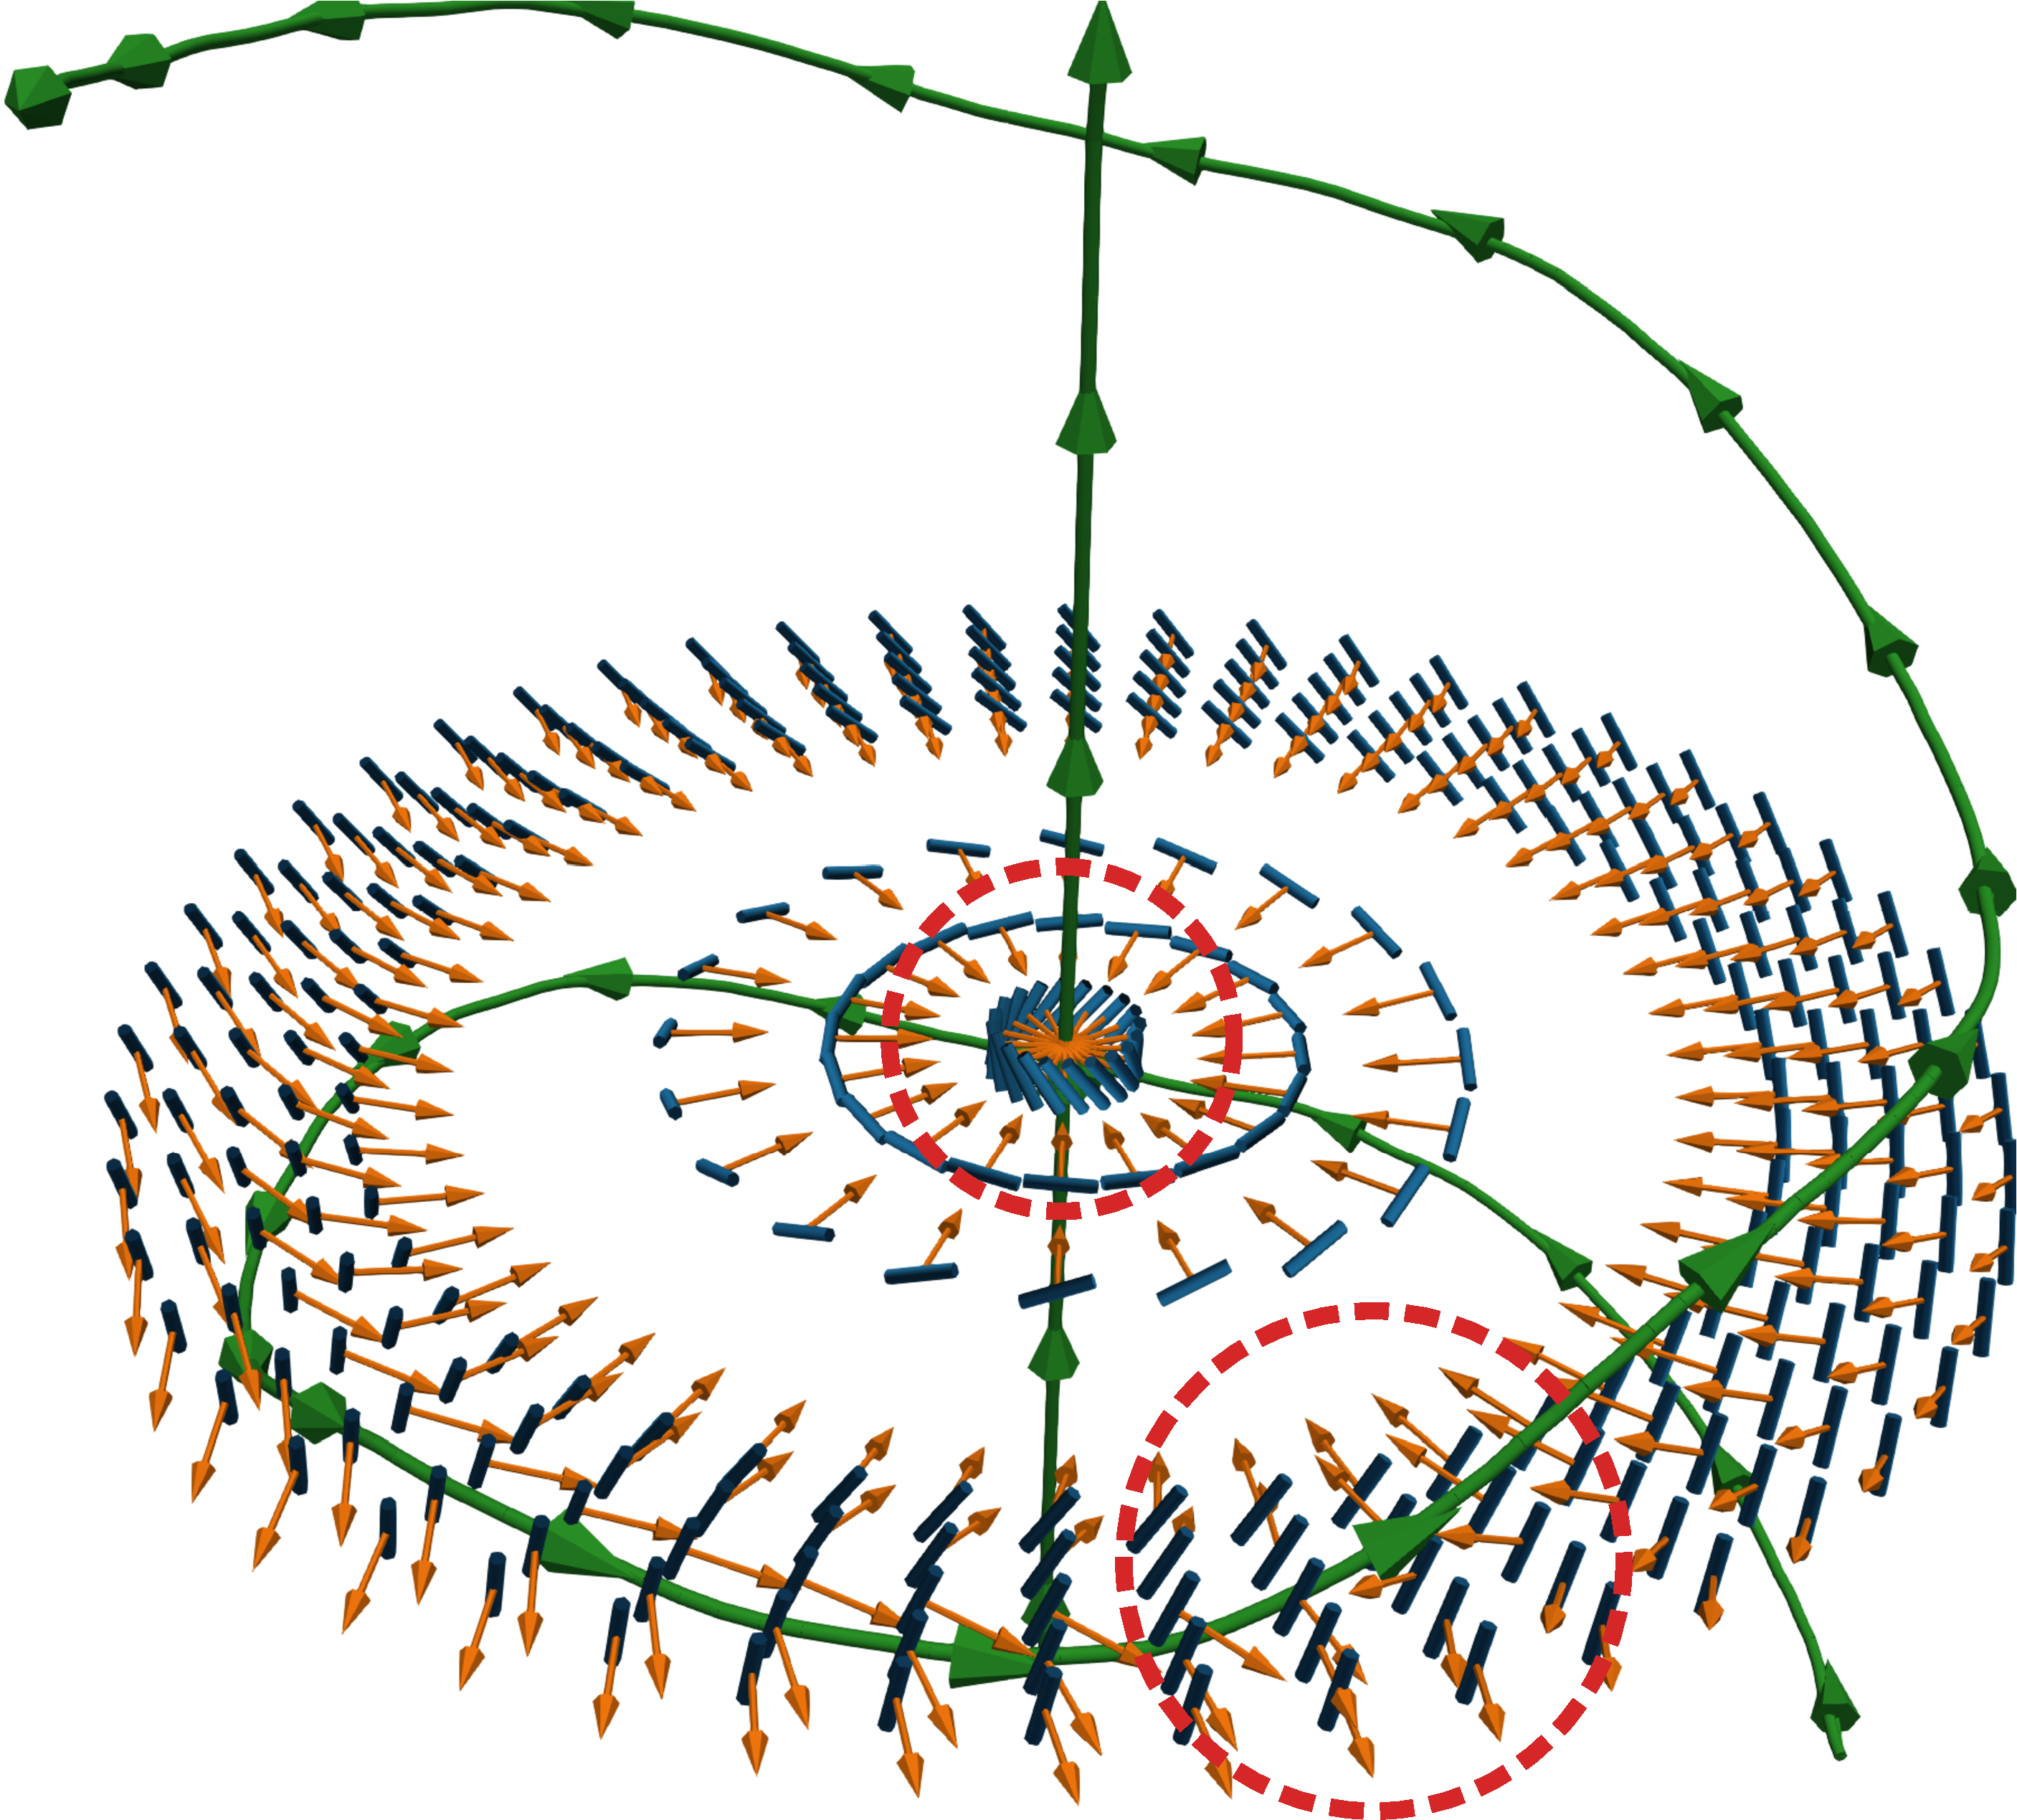
\includegraphics[width=0.5\textwidth]{\TwistBendFigures/TwistBendSkyrmion_annotated.pdf}
    \caption[Skyrmion tube in a twist-bend nematic.]{Skyrmion tube in a twist-bend nematic, with $\beta$ lines oriented by $\w j$ shown in green, and a cross section through the tube, which may be taken as a measuring surface, containing director (blue cylinders) and normalised bend vector (orange arrows). A signed intersection count of the $\beta$ lines piercing this surface gives $+2$, twice the Skyrmion number, consistent with \eqref{eq:GaussBonnetChern} --- these intersection points are highlighted in red circles, within which we see winding of the bend vector about its zeros.}
    \label{fig:TwistBendSkyrmion}
\end{figure}

In figure \ref{fig:TwistBendSkyrmion} we show a simulation of a stable Skyrmion tube in a twist-bend nematic, with director and bend shown on a single cross section through the tube, which may be taken as our surface $\Sigma$. The simulation is performed using a standard finite difference relaxation scheme applied to \eqref{eq:TwistBendFreeEnergy}. Extraction of $\beta$ lines is performed using a modified version of the methodology discussed in \S\ref{subsec:DefiningTracking} --- curves of minimal $|\w b|$ are traced by flowing along the vector field $\w j$, the theoretical tangent to the $\beta$ line, computationally corrected by minimisation in planes cross sectional to the $\beta$ line being traced out. We may extract the self-linking ribbons by constructing the solid angle framing for each component of our $\beta$ line (this is different to the framing for a linked set of $\beta$ lines --- the framing shown for the Whitehead link in figure \ref{fig:LocalStructure} has self-linking $+1$), pushing off a small distance (comparable to numerical gridspacing) along this framing to get a value of $\w b$, and then performing a second pushoff along that vector. 

The Skyrmion texture tends to the heliconical ground state \eqref{eq:TwistBendDirector}, \eqref{eq:TwistBendPolarisation} in the far field, and so on a cross section we see a constant far field director and bend vector --- these rotate as the cross section is varied along the tube. This far field behaviour allows us to compactify the boundary of $\Sigma$ as is usual when measuring Skyrmion number, considering it closed as in the discussion above. We see that our Skyrmion texture is punctured by two bend zeros, both positively co-oriented with the surface, giving a count of $+2$, twice the Skyrmion number, and telling us that the bundle $\xi$ has nontrivial Euler class. Note that summing $I^\xi_\beta$ gives $1-1=0$, a reflection of the fact that the director makes a half twist between the two zeros. We briefly note that the $\beta$ lines are consistently transverse to the director (although the central $\beta$ line is nongeneric), and that their handedness is in fact opposite to that of the director, both observations deserving of further study.

\subsection{$\beta$ lines and Hopfions}

In \S\ref{subsec:SkyrmionsAndHopfions} we gave an introduction to Hopfions, three dimensional analogues of Skyrmions characterised by an element $Q\in \pi_3(S^2)$ for an orientable director --- we described how they may be visualised using the Pontryagin-Thom construction, and provided experimental images of their realisation in cholesterics. It has been suggested that their stability in cholesterics (escaping Derrick's theorem) comes from the intrinsic lengthscale in the ground state given by the repeat length $\pi/q_0$ \citep{Ackerman2017}. This motivates their study in twist-bend nematics, which have a similar ground state and lengthscale \eqref{eq:q}. Hopfions are also the ideal test case for probing what topological information $\beta$ lines contain in addition to the Euler class $e(\xi)$. More specifically, all orientable three-manifolds are parallelisable \citep{Geiges2009}, and once a choice of basis has been made the director gives a map $\w n :M\rightarrow S^2$. The homotopy class of such a map is determined firstly by the Euler class $e(\xi)$ and secondly by a suitably defined element of $\pi_3(S^2)$. In a Hopfion $M=S^3$ and so $H^2(M)=0$, hence $e(\xi)\in H^2(M)=0$. Can the $\beta$ lines tell us the Hopf invariant $Q$?

In figure \ref{fig:Hopf} we show a Hopfion in a twist-bend nematic, simulated using fixed boundary conditions top and bottom and periodic boundaries in the horizontal plane, as is commonly used when simulating cholesteric Hopfions under confinement \citep{Ackerman2017}. In the vertical the simulation box is $2(2\pi/q)$, in the horizontal $8(2\pi/q)$. The texture itself is visualised using the Pontryagin Thom construction of \S\ref{subsec:HomotopyTheory} applied to the director. There are multiple constructions which explicitly realise such textures--- in the figure we simply rotate a Skyrmion texture around a central axis as described in~\citep{Sutcliffe2007}, giving a Hopfion with Hopf charge $Q=+1$, with the polarisation field $\w p$  then initialised to the bend of this director. More elaborate Hopfions may be constructed via rational maps \citep{Sutcliffe2007} as mentioned in \S\ref{sec:Introduction}, with preimages of the director then tracing the knotted zero set of a complex polynomial and generating Hopfions of larger $Q$. We briefly note that the Solid Angle function described in \S\ref{ch:Maxwell}, modified with a longitudinal phase as in \S\ref{subsec:WavefieldInitialisation}, can also be used as an alternate method for generating these knotted Hopfions, with control over curve geometry and cross sectional structure. 
\begin{figure}[htbp]
    \centering
    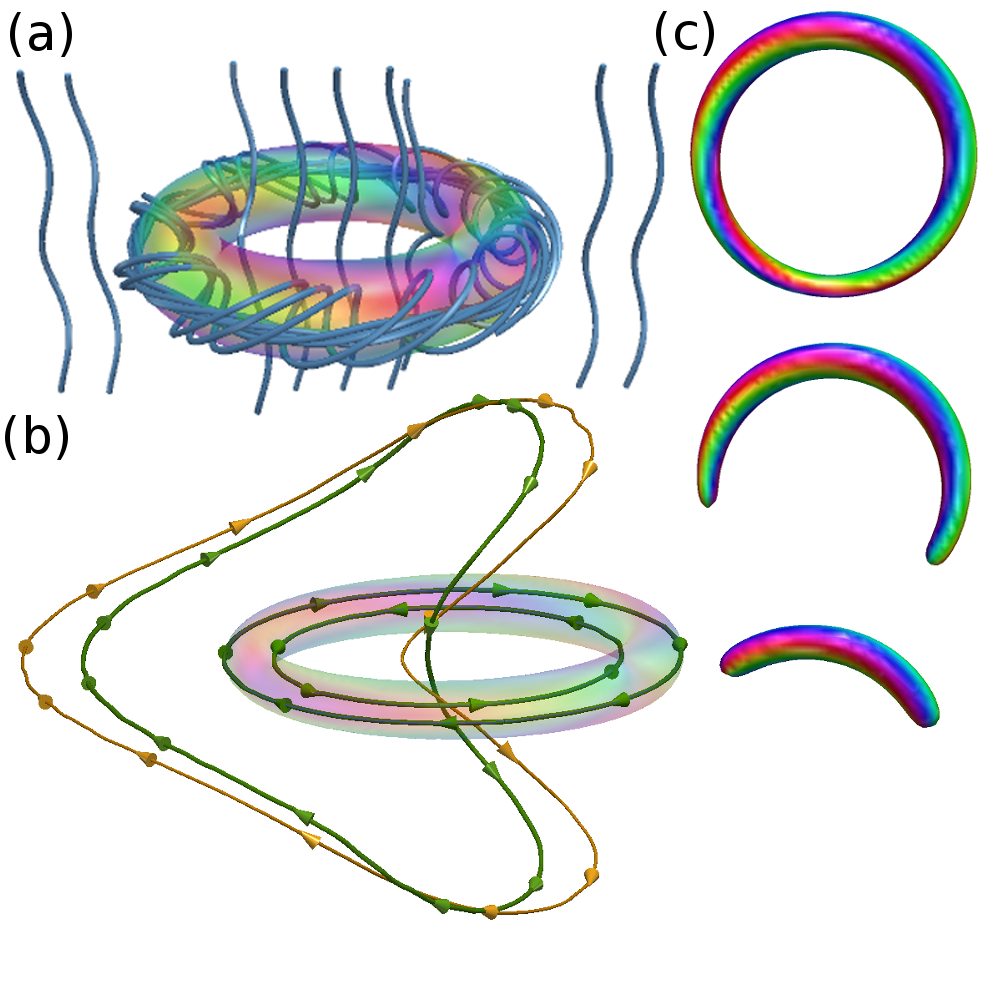
\includegraphics[width=0.8\textwidth]{\TwistBendFigures/hopf.png}
    \caption[Hopfion in a twist-bend nematic.]{$Q=+1$ Hopfion in a twist-bend nematic, visualised using the Pontryagin-Thom construction. (a) Integral curves of the director (blue tubes), showing a far field heliconical state with a reversal of helix handedness in the Hopfion core. (b) $\beta$ lines (green) in the Hopfion, oriented by $\w j$, with yellow curves denoting their self-linking ribbons (the azimuthal ribbons are simply displaced radially from their $\beta$ lines and are not shown for clarity). A count using \eqref{eq:BetaCount} gives $Q=+1$. (c) The Hopfion shown is not stable, but rather decays into two oppositely charged point defects (located at the tips of the PT surface shown) which then annihilate.  At the point of Hopfion decay, the bend zeros unlink and their self-linking decays to $0$.}
    \label{fig:Hopf}
\end{figure}

The Hopfion in figure~\ref{fig:Hopf} initially contains three $\beta$ lines, shown in figure~\ref{fig:Hopf}(b), each oriented by $\w j$ and linked with one another. In addition, the central $\beta$ line has self-linking $+1$ with the remaining two having self-linking number $0$. Although not shown in figure \ref{fig:Hopf}, constructing a Hopfion with $Q=-1$ gives a mirror image, with all linking and self-linking numbers reversed. This Hopfion is not stable --- it decays into two point defects which then annihilate, as shown in figure \ref{fig:Hopf}(c), a well known decay channel for Hopfions \citep{Chuang1991}. At the point of Hopfion decay, its $\beta$ lines unlink and their self-linking changes to $0$. Based on simulations of this type, we conjecture that a result analogous to the helicity count of \eqref{eq:HelicityCount} holds for these $\beta$ lines:
\begin{equation}
    Q = \sum_{i,j, i\neq j}Lk(\beta_i,\beta_j) + \sum_{i} SL(\beta_i). 
    \label{eq:BetaCount}
\end{equation}
Applying this count to figure \ref{fig:Hopf} gives a change from $Q=+1$ --- the linking numbers cancelling and the self-linking giving $+1$ --- to $Q=0$ as the Hopfion decays. For its mirror image, it would be from $Q=-1$ to $Q=0$. As well as simulation evidence, there  is good theoretical reason for conjecturing \eqref{eq:BetaCount}. It appears to coincide with a prescription for computing the $\Theta$ invariant of three-manifolds \citep{Gompf1998}, which must relate to the Hopf invariant on $S^3$. Further, a result partially capturing this structure has been demonstrated for umbilics in \citep{Machon2016b}. Nevertheless, we do not currently have a self-contained proof, and the issue certainly deserves further study. 

\section{Discussion}
\label{sec:Discussion}

As well as a self-contained proof of \eqref{eq:BetaCount}, several other issues deserve further study. Firstly, although the Hopfion presented in figure \ref{fig:Hopf} (and those in other simulations we have performed) decays, it is perhaps premature to conclude that Hopfions are inherently unstable in twist-bend nematics (in contrast to cholesterics). Our initialisation methodology is coarse --- we should not assume that simply constructing a director with the desired Hopf invariant and then setting the polarisation to director bend is an appropriate method, especially given the metastability of these states in cholesterics. Progress here likely starts with further study of the geometry of stable Hopfions in cholesterics \citep{Ackerman2017}.

The second issue was raised at the end of \S\ref{sec:Elements}. The bend is a canonically given section of $\xi$, but it cannot be varied independently of $\w n$, suggesting it may contain more information than can be captured in an arbitrary section. Let us briefly consider the bend of a texture on a two-manifold, in particular $T^2$; a discussion of the geometry of bend in two dimensions may be found in~\citep{Niv2018}, although not of its topology. Homotopy classes of maps $T^2 \rightarrow S^2$ are given by the degrees of the meridional and longitudinal restrictions, however the bundle $\xi$ is trivial here, and an arbitrary section should contain no information about these degrees. By contrast, based on preliminary simulations and a direct homotopy argument, it appears that a count of oriented bend zeros (again lines on $T^2$) along any meridian or longitude computes exactly these degrees. In summary, the geometry and topology of bend contain many fascinating basic questions, which currently appear unanswered.



 \begin{subappendices}
 \input{Chapters/TwistBendAppendix.tex}
 \end{subappendices}

                            %% More chapters.
%!
%! There are a few variations of reference
%\begin{verbatim}\citet[chap. 2]{ballentine82}|
%\end{verbatim}
%for a textual one, as \citet[chap. 2]{ballentine82}.\\
% \\
%\begin{verbatim}\citep{abraham_etal}
% \end{verbatim}
% for a parenthetical citation \citep{abraham_etal},\\
%
% \begin{verbatim}\citep*{MTW}
% \end{verbatim}
% for a full list of authors use a * parenthetical citation \citep*{MTW},\\
% \\
%!!!!!!!!!!!!!!!

%  \appendix                            %% this will do the appendices
%  \input{app1.tex}
%  \chapter{listing of Fred's program}
%  \input{app2.tex}

\bibliographystyle{plainnat}

\bibliography{ThesisBibliography}            %% Start your bibliography here;
                                 %! with sample.bib as your bibliography file. You can
                               %% also use:
                %! \begin{thebibliography}
                %!    \bibitem{etc....
                %! \end{thebibliography}
                               %% to generate your bibliography.

%\begin{thesisauthorvita}             %% Write your vita here; it can be
%                                     %% anything in LaTeX2e par-mode.
%\end{thesisauthorvita}               %%

\end{document}                       %% Done.
